\documentclass{nthu_thesis}

\geometry{
  a4paper,
  left=3cm,
  right=3cm,
  top=3cm,
  bottom=3cm,
  bindingoffset=0mm,
  headheight=0pt,
  headsep=0pt,
  footskip=18pt
}
\setlength{\hoffset}{0pt}
\setlength{\oddsidemargin}{15.5pt}
\setlength{\marginparwidth}{0pt}
\setlength{\marginparsep}{0pt}

%%% Customization — packages required by the migrated thesis content %%%
% nthu_thesis.cls 已內建 amsmath / amssymb / booktabs / caption / subcaption /
% graphicx / hyperref / biblatex(style=ieee) / multirow / siunitx；下列為舊內文用到、
% 但新 cls 未載入的補強。
\usepackage[expansion=false]{microtype} % 改善排版；CJK 場景關閉字距擴張
\usepackage{array}                      % tabularx column helpers
\usepackage{tabularx}                   % full-width tables
\usepackage[ruled]{algorithm2e}         % algorithm environment & List of Algorithms
\usepackage{placeins}                   % \FloatBarrier，避免 float 漂移到後面章節

% 章節內 caption 風格微調（不覆寫 nthu_thesis.cls 既有的 NTHU 標準）
\setlength{\emergencystretch}{2em}
\captionsetup[table]{skip=8pt}
\captionsetup[figure]{skip=6pt}

\begin{document}
\pagestyle{plain} % 預設樣式：頁碼置於頁尾置中，頁首為空
\begin{CJK}{UTF8}{bkai}

%%% Necessary fields for this thesis data %%%
\newcommand{\degreeZH}{碩}                    % 碩 (Master's) / 博 (Doctor's)
\newcommand{\degreeEN}{Master's Thesis}        % "Master's Thesis" / "Doctoral Dissertation"
\newcommand{\titleZH}{物理約束之稀疏感測器連續時間湍流場重建}
\newcommand{\titleEN}{Physics-Constrained Continuous-Time Reconstruction of Turbulent Flows from Sparse Sensors}
\newcommand{\instituteZH}{工程與系統科學研究所乙組}
% instituteEN 原為「Department of Engineering and System Science, Group B」共 50 字元，
% 在封面 \Large 字級 + 含 "Dept. / Grad. Inst.:" prefix 下會溢出 textbox。
% 縮為「Engineering and System Science, Group B」（去除 prefix label 已表達的
% "Department of" 重複資訊）即可一行排下。
\newcommand{\instituteEN}{Engineering and System Science, Group B}
\newcommand{\studentID}{113011527}
\newcommand{\studentZH}{李駿毅}
\newcommand{\studentEN}{JunYi Li}
\newcommand{\advisorZH}{林洸銓}
\newcommand{\advisorEN}{Kuang C. Lin}
\newcommand{\yearZH}{115}     % 民國年
\newcommand{\monthZH}{6}      % 民國月
\newcommand{\yearEN}{2026}    % 西元年
\newcommand{\monthEN}{June}   % 西元月


\begin{titlepage}
\newgeometry{a4paper,left=2.54cm,right=3.18cm,top=3.18cm,bottom=2.54cm}  %NTHU cover page setting
% 封面對稱用：main.tex 把 \oddsidemargin 設了 15.5pt 補裝訂邊，但封面要對稱置中，
% 在這頁先 reset 為 0；titlepage 結束後 main.tex 的設定會自動重新生效。
\setlength{\oddsidemargin}{0pt}
\setlength{\evensidemargin}{0pt}

 \begin{CJK*}{UTF8}{bkai}
\begin{spacing}{1.3}
    \begin{center}
       \Huge
        國\hspace{1em}立\hspace{1em}清\hspace{1em}華\hspace{1em}大\hspace{1em}學\\
        National Tsing Hua University\\
        \vspace{0.6cm}
        \degreeZH~~~士~~~論~~~文\\
        \degreeEN

    \vspace{2em}  %for controlling veretical space (was 3em; reduced to fit single page)
    \LARGE
        \titleZH\\[0.4em]
        % 題目超過一行時用 minipage 讓 \titleEN 自動 wrap，避免被 textbox 右邊裁切；
        % 寬度設 0.9\textwidth 在置中對稱下視覺一致。
        \begin{minipage}{0.9\textwidth}
            \centering\titleEN
        \end{minipage}\\
    \vspace{2em} %for controlling veretical space (was 3em)

   \Large

%  \setlength\tabcolsep{3pt} % default: 6pt
\renewcommand{\arraystretch}{1.3} % default value is 1.0
      \begin{tabular}{ l }  %l: Left-aligned column.
        系所別：~\instituteZH\\
        Dept.~/~Grad. Inst.:\hspace{0.5em}\instituteEN\\
        學號~ Student ID:\hspace{0.5em}\studentID\\
        研究生~Author：\hspace{0.5em}\studentZH\hspace{0.5em}\studentEN\\
        指導教授~Advisor：\hspace{0.5em}\advisorZH\hspace{0.5em}\advisorEN
    \end{tabular}\\

   \vfill   % was \vspace{3em}; \vfill 把日期推到頁底，避免內容塞到第二頁

    中~~華~~民~~國~~\zhdigits{\yearZH}~年~~\zhdigits{\monthZH}~月\\
    \monthEN~\yearEN
     
     \end{center}
\end{spacing}
\end{CJK*}
\end{titlepage}




% TODO: 正式繳交（NTHU Library 送審）前補回「扉頁 + 內封」：
%       裝訂後對應「外封 → 空白扉頁 → 內封(title page)」三層結構。
%       電子試讀 / 校內 working draft 可不放；library 送審時把下方 % 拿掉。
%
% \newpage
% \null
% \thispagestyle{empty}
% \newpage
% 
\begin{titlepage}
\newgeometry{a4paper,left=2.54cm,right=3.18cm,top=3.18cm,bottom=2.54cm}  %NTHU cover page setting
% 封面對稱用：main.tex 把 \oddsidemargin 設了 15.5pt 補裝訂邊，但封面要對稱置中，
% 在這頁先 reset 為 0；titlepage 結束後 main.tex 的設定會自動重新生效。
\setlength{\oddsidemargin}{0pt}
\setlength{\evensidemargin}{0pt}

 \begin{CJK*}{UTF8}{bkai}
\begin{spacing}{1.3}
    \begin{center}
       \Huge
        國\hspace{1em}立\hspace{1em}清\hspace{1em}華\hspace{1em}大\hspace{1em}學\\
        National Tsing Hua University\\
        \vspace{0.6cm}
        \degreeZH~~~士~~~論~~~文\\
        \degreeEN

    \vspace{2em}  %for controlling veretical space (was 3em; reduced to fit single page)
    \LARGE
        \titleZH\\[0.4em]
        % 題目超過一行時用 minipage 讓 \titleEN 自動 wrap，避免被 textbox 右邊裁切；
        % 寬度設 0.9\textwidth 在置中對稱下視覺一致。
        \begin{minipage}{0.9\textwidth}
            \centering\titleEN
        \end{minipage}\\
    \vspace{2em} %for controlling veretical space (was 3em)

   \Large

%  \setlength\tabcolsep{3pt} % default: 6pt
\renewcommand{\arraystretch}{1.3} % default value is 1.0
      \begin{tabular}{ l }  %l: Left-aligned column.
        系所別：~\instituteZH\\
        Dept.~/~Grad. Inst.:\hspace{0.5em}\instituteEN\\
        學號~ Student ID:\hspace{0.5em}\studentID\\
        研究生~Author：\hspace{0.5em}\studentZH\hspace{0.5em}\studentEN\\
        指導教授~Advisor：\hspace{0.5em}\advisorZH\hspace{0.5em}\advisorEN
    \end{tabular}\\

   \vfill   % was \vspace{3em}; \vfill 把日期推到頁底，避免內容塞到第二頁

    中~~華~~民~~國~~\zhdigits{\yearZH}~年~~\zhdigits{\monthZH}~月\\
    \monthEN~\yearEN
     
     \end{center}
\end{spacing}
\end{CJK*}
\end{titlepage}




\let\cleardoublepage=\clearpage % 抑制 book class 在章節之間自動插入空白頁

% TODO: 送審前補回三份 NTHU 必填表格的 \includepdf 與 \cftaddtitleline
%       (1) 學位論文授權書 — front/Authorized agreement.pdf (3 頁)
%       (2) 指導教授推薦書 — front/Advisor Approval Form.pdf (1 頁)
%       (3) 考試委員審定書 — front/Thesis Review Form.pdf (1 頁)
% 補回時，把下方 % 註解拿掉即可。實際 PDF 需替換為簽核完成的正式版。
%
% \cftaddtitleline{toc}{chapter}{學位論文授權書}{}
% \includepdf[pages=1-3, angle=0, fitpaper=true,
%        keepaspectratio, pagecommand={{\thispagestyle{empty}}},offset=-0.0cm 0.0cm]{./front/Authorized agreement.pdf}
% \includepdf[pages=1, angle=0, fitpaper=true,
%     keepaspectratio, pagecommand={{\thispagestyle{empty}}}]{./front/Advisor Approval Form.pdf}
% \cftaddtitleline{toc}{chapter}{指導教授推薦書}{}
% \includepdf[pages=1, angle=0, fitpaper=true,
%        keepaspectratio, pagecommand={{\thispagestyle{empty}}},offset=-0.0cm 0.0cm]{./front/Thesis Review Form.pdf}
% \cftaddtitleline{toc}{chapter}{考試委員審定書}{}

\frontmatter

%%% Abstract (English) %%%
\chapter*{Abstract}
\addcontentsline{toc}{chapter}{Abstract}
% English Abstract — migrated from legacy main.tex (lines 57-61)

Field-deployable turbulent-flow reconstruction must operate from sparse velocity sensors ($K \sim 10^2$) under low-latency inference budgets, with no Direct Numerical Simulation (DNS) full-field supervision for training. This work introduces \textbf{PI-CON} (\textbf{P}hysics-\textbf{I}nformed \textbf{C}ontinuous-time \textbf{O}perator \textbf{N}etwork), a Deep Operator Network (DeepONet) with a Closed-form Continuous-time (CfC) sensor encoder and a distance-biased cross-attention readout, trained on Navier--Stokes (NS) residuals and sensor measurements alone. Its CfC encoder reads the whole sensor stream in one pass, avoiding the sequential time-window training high-Reynolds physics-informed networks rely on; the work then quantifies how the sensing configuration (count, placement, and noise) governs reconstruction quality.

On the 2D Kolmogorov flow at $Re=10\,000$ with $K=100$ sensors, PI-CON reconstructs at engineering grade under sensor-plus-physics supervision: over five random seeds it attains a Kinetic Energy (KE) relative error of $\mathbf{5.71 \pm 0.11\%}$, with the energy-dominant low-wavenumber band within single-digit error; once trained, it reconstructs any query point in a single forward pass without re-solving the flow. The same architecture extends to $Re=10^6$ ($6.10\%$ KE relative error at $K=200$ sensors).

The sensing configuration then sets resolution and reliability, not feasibility. The mid-high-wavenumber band ($k > k_{\max}^{\rm sensor}\approx 5.64$) is limited by the $K=100$ sensor information: $\sqrt{K/\pi}$ is a Nyquist-like scale, and the effective bandwidth is set by conditioning and noise rather than by an architectural shortfall. A $K$-scaling sweep ($K \in \{100, 200, 400\}$) confirms the cutoff moves as the $\sqrt{K/\pi}$ scale predicts. Placement fixes only sensor locations; the values are sampled from a DNS field that stands in for the experimentally inaccessible real-world flow, never the full field, which supervises nothing. Across three placement strategies (a DNS-pivot oracle, a DNS-free Large-Eddy-Simulation (LES) placement that needs no DNS for siting, and random) reconstruction stays engineering-grade, with placement variance about six times training stochasticity. Additive sensor noise up to $10\%$ shifts KE by less than one percentage point.

\smallskip

\noindent\textbf{Keywords:} sparse sensors, turbulent-flow reconstruction, physics-informed neural networks, DeepONet, CfC, sensor placement, Kolmogorov flow

\setcounter{page}{1}
\clearpage

%%% Abstract (Chinese) %%%
\chapter*{摘要}
\addcontentsline{toc}{chapter}{摘要}
% Chinese Abstract — migrated from legacy main.tex (lines 48-52)

工程現場之湍流場重建須自稀疏感測器（$K \sim 10^2$）進行低延遲推論，且訓練階段不能依賴 Direct Numerical Simulation（DNS）全場監督。本論文提出 \textbf{PI-CON}（\textbf{P}hysics-\textbf{I}nformed \textbf{C}ontinuous-time \textbf{O}perator \textbf{N}etwork），以 Deep Operator Network（DeepONet）任意點場解碼，結合 Closed-form Continuous-time（CfC）連續時間感測器編碼器與距離偏置 cross-attention。PI-CON 僅以感測器量測與 Navier--Stokes（NS）residual 訓練；其 CfC 編碼器一次讀入整段感測時序，避開高雷諾數物理約束網路常用之時間窗順序訓練。本研究並量化 sensing configuration（數量、位置與噪聲）如何決定重建品質。

於 $Re=10\,000$ 之 2D Kolmogorov 受迫湍流、$K=100$ 感測器下，PI-CON 在純感測器加物理約束的監督下達到工程目標：經五個 random seed，其 Kinetic Energy（KE）相對誤差為 $\mathbf{5.71 \pm 0.12\%}$，energy-dominant 低波數段維持單位數相對誤差。訓練完成後，模型可於單次前傳查詢任意時空點，無需重新求解流場。同架構可延伸至 $Re=10^6$（於 $K=200$ 感測器達 KE 相對誤差 $6.10\%$）。

sensing configuration 決定解析度與可靠度，而非可行性。中高頻段（$k > k_{\max}^{\rm sensor}\approx 5.64$）受 $K=100$ 感測器資訊量限制：取樣密度條件（每個可解析模態至少需一個取樣）將頻帶邊界定於此尺度，有效頻寬則由 conditioning 與噪聲決定，而非架構不足；$K$ 由 $100$ 增至 $200$、$400$ 之掃描證實 cutoff 隨感測器數之平方根移動。佈點僅決定感測器位置；感測值取自一個代表實驗上無法取得之真實流場的 DNS 場，但全場從不參與訓練監督。在三種佈點策略（DNS-pivot oracle、不需 DNS 之 Large-Eddy Simulation（LES）佈點、隨機佈點）下，重建皆維持在工程目標內；佈點變異約為訓練隨機性之六倍，加性感測器噪聲至 $10\%$ 對 KE 之影響仍不到一個百分點。

\smallskip

\noindent\textbf{關鍵字：}稀疏感測器、湍流場重建、物理約束神經網路、DeepONet、CfC、感測器佈點、Kolmogorov 流場

\clearpage

%%% Acknowledgements %%%
\chapter*{Acknowledgements}
\addcontentsline{toc}{chapter}{Acknowledgements}
The acknowledgements section expresses gratitude to individuals and entities who supported the research and dissertation process, reflecting academic courtesy and personal appreciation.
    
\textbf{Content Elements}
\begin{itemize}
    \item Acknowledge indirect contributors, such as funding agencies, institutions providing equipment, or colleagues involved in discussions.
    \item Recognize assistants in research execution, such as lab technicians, research assistants, or peers.
   \item Optionally thank personal supporters who aided your academic or personal growth, such as parents, family, or friends.

\end{itemize}

\bigskip
\textbf{Writing Tips}
\begin{itemize}
   \item Adopt a sincere, slightly personal tone while maintaining brevity and professionalism, avoiding excessive length or emotional language.
   \item Organize by significance, starting with advisors and funding bodies, followed by personal supporters.
   \item Ensure key contributors are included without listing every individual involved.
    \item Check institutional guidelines, as some require acknowledgements at the end or on a separate page.

\end{itemize}



\clearpage

%%% Front matter listings %%%
\begingroup
\sloppy
\hbadness=10000
\vbadness=10000
\hfuzz=10pt
\vfuzz=10pt

\tableofcontents
\addcontentsline{toc}{chapter}{Contents}
\clearpage

\listoffigures
\addcontentsline{toc}{chapter}{List of Figures}
\clearpage

\listoftables
\addcontentsline{toc}{chapter}{List of Tables}
\clearpage
\endgroup

%%% Abbreviations and Notation %%%
\chapter*{Abbreviations and Notation}
\addcontentsline{toc}{chapter}{Abbreviations and Notation}
% Abbreviations and Notation — migrated from legacy main.tex (lines 83-160)
% 註：原本以 % main.tex 已負責章節骨架（
\noindent\textbf{Abbreviations}
\vspace{0.5em}

% \renewcommand{\arraystretch} 在 group 內設定以避免全域副作用；
% 0.72 ≈ 1/1.8 將 NTHUthesis 的 1.8 倍行距壓回接近 1.0 倍。
{\renewcommand{\arraystretch}{0.72}%
% \noindent 抑制段首縮排：\textwidth 寬的 tabularx 若帶 parindent 會被推出右邊界
% （overfull ~23pt），與下方 Notation 表的 \noindent 對齊處理。
\noindent\begin{tabularx}{\textwidth}{@{}>{\raggedright\arraybackslash}p{2.8cm} >{\raggedright\arraybackslash}X@{}}
PI-CON   & Physics-Informed Continuous-time Operator Network (this work) \\
PINN(s)  & Physics-Informed Neural Network(s) \\
DeepONet & Deep Operator Network \\
FNO      & Fourier Neural Operator \\
CfC      & Closed-form Continuous-time network \\
LNN      & Liquid Neural Network \\
LTC      & Liquid Time-Constant network \\
RFF      & Random Fourier Features \\
RWF      & Random Weight Factorization \\
GradNorm & Gradient-Norm based loss balancing \\
SOAP     & Shampoo with Adam in the Preconditioner's eigenbasis \\
QRCP     & QR factorization with Column Pivoting \\
QR-pivot & Sensor placement based on QRCP on POD modes \\
POD      & Proper Orthogonal Decomposition \\
DMD      & Dynamic Mode Decomposition \\
MLP      & Multi-Layer Perceptron \\
ANOVA    & Analysis of Variance \\
SVD      & Singular Value Decomposition \\
DNS      & Direct Numerical Simulation \\
LES      & Large-Eddy Simulation \\
RANS     & Reynolds-Averaged Navier--Stokes \\
NS       & Navier--Stokes \\
PDE      & Partial Differential Equation \\
CS       & Compressed Sensing \\
RIP      & Restricted Isometry Property \\
CFD      & Computational Fluid Dynamics \\
KE       & Kinetic Energy \\
EMA      & Exponential Moving Average \\
MAPE     & Mean Absolute Percentage Error \\
MSE      & Mean Squared Error \\
ETDRK4   & Exponential Time Differencing Runge--Kutta 4 \\
\end{tabularx}}

\par\addvspace{1em}
\noindent\begin{minipage}{\textwidth}
\textbf{Notation}\par\vspace{0.5em}
\renewcommand{\arraystretch}{0.72}%
\begin{tabularx}{\textwidth}{@{}>{\raggedright\arraybackslash}p{3.2cm} >{\raggedright\arraybackslash}X@{}}
$\Omega$ & Spatial domain, $[0,1\,\mathrm{m}]^2$ for 2D Kolmogorov flow (periodic) \\
$\mathbf{x} = (x,y)^T$ & Spatial coordinates (m) \\
$t \in [0, T]$ & Time (s), with horizon $T = 5$\,s in the main experiments \\
$\mathbf{u}(\mathbf{x},t) = (u,v)^T$ & Velocity field (m/s) \\
$p(\mathbf{x},t)$ & Pressure field (model-internal; not data-supervised), m$^2$/s$^2$ \\
$\omega(\mathbf{x},t)$ & 2D vorticity, $\omega = \partial_x v - \partial_y u$ (1/s; diagnostic only) \\
$\nu$ & Kinematic viscosity, $\nu = U L / Re$ (m$^2$/s); $\nu = 10^{-4}$\,m$^2$/s at $Re=10\,000$ \\
$Re$ & Reynolds number based on $L = 1$\,m and $U = 1$\,m/s \\
$k_f$ & Forcing wavenumber (1/m) in Kolmogorov flow ($k_f=2$\,m$^{-1}$ in main runs) \\
$\mathbf{f}$ & Body forcing (m/s$^2$), $\mathbf{f} = (A\sin(2\pi k_f y), 0)^T$ with $A = 0.1$\,m/s$^2$ \\
$K$ & Number of sparse velocity sensors \\
$\mathcal{S} = \{\mathbf{x}_s\}_{s=1}^K$ & Sensor locations \\
$s \in \{1,\dots,K\}$ & Sensor index; paired with the query index $q$ in $\mathbf{r}_{qs}$, $A_{qs}$ \\
$q$ & Query index, labelling an evaluation point $(\mathbf{x}_q, t_q)$ \\
$N_{\rm run} = 1024\times 1024$ & DNS solver run grid \\
$N = 256\times 256$ & Stored DNS snapshot grid (downsampled $\times 4$; used as the training reference) \\
$N_t$ & Number of sensor sampling time stamps \\
$\mathbf{D}$ & Sensor observations $\{u,v\}$ at $\mathcal{S}\times\{t_n\}_{n=1}^{N_t}$ \\
$\boldsymbol{\Psi}^{\text{branch}}, \boldsymbol{\Psi}^{\text{trunk}}$ & DeepONet branch / trunk basis vectors $\in\mathbb{R}^{3\times R}$ (\S\ref{subsec:operator_fusion}) \\
$d_{\text{model}}$ & Hidden width of CfC encoder \& decoder in the main configuration \\
$d_{\text{emb}}$ & Fourier embedding dimension \\
$d_{\text{hidden}}$ & Trunk MLP hidden width \\
$d_t$ & Time-projection embedding dim ($=16$) \\
$R$ & DeepONet operator rank ($=d_{\text{model}}$ default) \\
$L_s, L_a, L_t, L_q$ & Layer counts: spatial encoder / token attention / temporal CfC / trunk MLP \\
$h_s(t) \in \mathbb{R}^d$ & CfC token state for sensor $s$ at time $t$ \\
$\theta$ & Trainable network parameters \\
$c \in \{0,1,2\}$ & Channel index for $(u, v, p)$ in the operator output \\
$\sigma$ & Disambiguated locally (singular value, std, CfC sigmoid, or envelope band) \\
$\mathcal{L}_{\text{data}}$ & Sensor-MSE loss on $u,v$ \\
$\mathcal{L}_{\text{NS},u}, \mathcal{L}_{\text{NS},v}$ & Momentum residuals (Eulerian form) \\
$\mathcal{L}_{\text{cont}}$ & Continuity residual $\partial_x u + \partial_y v$ \\
$\mathbf{k}, k$ & Ordinary (cyclic) wavenumber vector and its magnitude $k=\vert\mathbf{k}\vert$ (1/m); integer-valued on the unit box (\S\ref{subsec:spectrum_definition}). Denotes a wavenumber throughout; sensors are indexed by $s$ \\
$E(k)$ & Radial energy spectrum, m$^3$/s$^2$, on unit-width shells $\Delta k = 1$\,m$^{-1}$, Eq.~\eqref{eq:radial_spectrum} \\
$k_{\max}^{\rm sensor}$ & Sensor-count sampling band edge $\sqrt{K/\pi}$ (1/m), Eq.~\eqref{eq:sensor_nyquist}; $\approx 5.64$\,m$^{-1}$ at $K=100$ \\
$k_{\max}$ & Angular dealiased grid maximum wavenumber (rad/m), used only in the Pope criterion $k_{\max}\eta$ \\
$\Vert\cdot\Vert_2, \Vert\cdot\Vert_\infty$ & $L_2$ and $L_\infty$ norms over the spatial grid \\
\end{tabularx}
\end{minipage}

\clearpage

% Contents of Thesis
\mainmatter
\pagestyle{plain}

\chapter{Introduction}
\label{ch:intro}

\section{Background}
\label{sec:intro_background}

Reconstructing a continuous turbulent flow field from sparse point measurements arises in aerospace boundary-layer estimation, wind-farm wake monitoring, biomedical Particle Image Velocimetry (PIV) slice fusion, and active flow control. Field deployment in these settings shares three operational constraints. First, instruments report at most $\sim 10^2$ point measurements, whereas the field to be reconstructed carries far more degrees of freedom (of order $10^5$ on the $256^2$ grid used here, growing as $Re^{9/4}$ for a three-dimensional simulation at high Reynolds number~\cite{Pope2000}). Second, no offline DNS reference is available at training or inference. Third, low-latency inference from the live sensor feed is required for active flow control.

Approaches to estimating a flow field from limited measurements have evolved through three broad stages. Classical reduced-order models compress the field onto a handful of modes identified offline and place sensors to condition that basis, while variational and ensemble data assimilation~\cite{Asch2016DA} fuse measurements with a forward solver; both rely on either an offline trajectory or repeated solver calls. Supervised deep-learning surrogates~\cite{VinuesaBrunton2022NCS} learn the measurement-to-field map directly in a single forward pass, but require paired full-field simulation data. Physics-informed methods relax that data demand: physics-informed neural networks~\cite{Raissi2019JCP} embed the PDE residual as a training constraint, neural operators~\cite{Lu2021NMI} learn mesh-free solution operators queryable at any coordinate, and physics-informed neural operators~\cite{Li2021PINO} combine the two, yet these target mostly forward or dense-input problems, not the sparse-sensor inverse setting. No line jointly satisfies the field-deployable constraints above (sensor-only training without a full reference field, and low-latency inference from a sparse live feed), which is the regime this work targets; \S\ref{sec:literature} examines each line in turn.

The difficulty underlying every stage has a quantitative anchor: reconstructing $N$ field values from $K \ll N$ point measurements is an under-determined inverse problem, and compressed-sensing theory bounds when exact recovery is achievable. The compressed-sensing bound~\cite{Donoho2006, Candes2006},
\begin{equation}
    \label{eq:cs_bound}
    M \;\ge\; C_0 \, s \, \log_2(N/s),\qquad C_0\in[1,2],
\end{equation}
where $M$ is the number of measurements, $s$ the number of significant wavelet coefficients, and $N$ the grid size, places the exact-recovery threshold for sparse signals on a $256^2$ grid an order of magnitude above the typical $\sim 10^2$ sensor budget. Engineering deployment at $K \sim 10^2$ therefore does not seek pointwise exact recovery; it asks how much of the energy-dominant flow structure can be reconstructed within this budget under a low-latency inference constraint, and whether the residual error is bounded by the sensor budget or by the chosen architecture.\label{sec:underdetermined}

\section{Literature Review}
\label{sec:literature}

This section reviews seven research lines on sparse-sensor turbulent-flow reconstruction, ordered from classical to recent and from algorithm-only to physics-aware (Table~\ref{tab:lit_summary}). \S\ref{sec:gap} consolidates the methodological limitations into four research gaps.

\begin{table}[!htbp]
    \centering
    \caption{Seven research lines relevant to sparse-sensor turbulent-flow reconstruction and the structural limitation that blocks each from addressing the engineering-deployable setting on its own.}
    \label{tab:lit_summary}
    \footnotesize
    \setlength{\tabcolsep}{3pt}
    \renewcommand{\arraystretch}{1.1}
    \begin{tabularx}{\textwidth}{
        >{\raggedright\arraybackslash}p{2.0cm}
        >{\raggedright\arraybackslash}p{3.4cm}
        >{\raggedright\arraybackslash}X
        >{\raggedright\arraybackslash}p{1.9cm}
        >{\raggedright\arraybackslash}p{2.3cm}
    }
    \toprule
    \textbf{Research line} & \textbf{Representative works} & \textbf{Main contribution} & \textbf{Supervision regime} & \textbf{Structural limitation} \\
    \midrule
    Reduced-Order Model (ROM) \& sparse identification
    & POD~\cite{Sirovich1987POD}; DMD~\cite{Schmid2010DMD}; SINDy~\cite{Brunton2016SINDy}; QR-pivot~\cite{Manohar2018PNAS}
    & Compress the field onto a low-rank basis identified offline.
    & Offline DNS trajectory
    & Needs offline trajectory; linear basis. \\
    \midrule
    Data assimilation
    & 4D-Var, EnKF~\cite{Asch2016DA}; B-PINN~\cite{Yang2021JCP}
    & Bayesian state estimation against a forward solver and noise model.
    & Forward solver + sensor
    & Adjoint cost; HMC scaling at high $Re$. \\
    \midrule
    Deep super-resolution / ROM
    & Fukami, 2019~\cite{Fukami2019JFM}; Maulik, 2021~\cite{Maulik2021NN}
    & Learn an upsampling map or latent dynamics from paired snapshots.
    & Paired DNS supervision
    & Paired DNS required; no PDE consistency. \\
    \midrule
    Operator learning
    & DeepONet~\cite{Lu2021NMI}; FNO~\cite{Li2021FNO}; Galerkin/OFormer~\cite{Cao2021Galerkin, Li2023OFormer}
    & Learn a mapping between whole functions (e.g.\ forcing $\to$ solution field): a branch sub-network reads the input function, a trunk evaluates the output at any query coordinate.
    & Paired field supervision
    & Dense-input forward operators; not sparse inverse. \\
    \midrule
    Stabilized PINNs
    & Wang 2022~\cite{wang2022respectingcausality}, 2024~\cite{Wang2024JMLR}, 2025~\cite{wang2025gradientalignmentpinns}
    & Causal weighting, PirateNet, and SOAP make stiff high-$Re$ training tractable.
    & PDE-only (no sensor)
    & Forward focus; MLP backbone underuses the sensor trajectory. \\
    \midrule
    Liquid NN / continuous-time
    & LTC~\cite{Hasani2021LTC}; CfC~\cite{Hasani2022CfC}; Neural/Latent ODE~\cite{Chen2018NODE, Rubanova2019LatentODE}
    & ODE-based and closed-form RNN dynamics for irregular sampling.
    & Paired sequence supervision (no PDE)
    & Not applied to PDE or fluid reconstruction. \\
    \midrule
    Sparse-sensor with physics
    & Mo \& Magri, 2025~\cite{Mo2025PRF}; Kelshaw, 2022~\cite{Kelshaw2022PISR}; Parfenyev, 2024~\cite{Parfenyev2024PINN}; SHRED~\cite{Williams2024SHRED}; Senseiver~\cite{Senseiver2023}
    & Most recent sensor-only-with-PDE or DNS-paired architectures; the first three use sensor measurements plus the PDE only.
    & Sensor-only with PDE (Mo \& Magri, Kelshaw, Parfenyev) vs.\ DNS-paired with priors (others)
    & Sensor-only-with-PDE works are grid-based at $Re\!\lesssim\!10^3$; no query-anywhere continuous-time operator variant at high $Re$. \\
    \bottomrule
    \end{tabularx}
\end{table}
\FloatBarrier

\paragraph{Classical reduced-order and data-assimilation methods.}
Proper Orthogonal Decomposition (POD)~\cite{Sirovich1987POD}, Dynamic Mode Decomposition (DMD)~\cite{Schmid2010DMD}, and sparse identification~\cite{Brunton2016SINDy} compress the field onto a low-rank linear basis, with QR-pivot~\cite{Manohar2018PNAS} or Q-DEIM~\cite{Drmac2016SISC} placement conditioning that basis; all require an offline DNS trajectory whose cost grows steeply with Reynolds number. Variational and ensemble Bayesian assimilation~\cite{Asch2016DA} instead fuse measurements with a forward solver, trading trajectory cost for repeated adjoint or sampling calls. Neither delivers the fast, reference-free inference a live control loop demands.

\paragraph{Learned reconstruction trained on full fields.}
A second line learns the measurement-to-field map directly. Convolutional super-resolution~\cite{Fukami2019JFM} and recurrent-autoencoder reduced-order models~\cite{Maulik2021NN} upsample or evolve a latent from paired snapshots; more recent sensor-input designs improve accuracy: SHRED~\cite{Williams2024SHRED} regresses the full state from a sensor time series through a shallow decoder, Senseiver~\cite{Senseiver2023} and the Energy Transformer~\cite{EnergyTransformer2025} use cross-attention or associative-memory inpainting, and FLRNet~\cite{FLRNet2024} learns a Fourier-feature variational autoencoder. Whatever the accuracy, every one of these is supervised by a full reference field (as a decoder target, a perceptual or variational loss, or masked-patch inpainting) and imposes no PDE, so none can be trained where no DNS field exists (Gap~1).

\paragraph{Operator learning for partial differential equations.}
Operator networks learn mappings between whole functions. DeepONet~\cite{Lu2021NMI} factorises the operator into a branch that reads the input function and a trunk that evaluates any query coordinate~\cite{ChenChen1995} (the query-anywhere readout adopted in this work), while the Fourier Neural Operator (FNO)~\cite{Li2021FNO} and attention variants~\cite{Cao2021Galerkin, Li2023OFormer} apply global spectral or kernel mixing. These are demonstrated as dense-input forward operators: the branch expects its input function sampled on a fixed dense grid (the FNO spectral mixing requires a regular mesh) rather than $\sim 10^2$ scattered points, and supervision is paired input--output fields. Even the physics-informed operator PINO~\cite{Li2021PINO} evaluates its residual on a grid. The sparse, scattered-sensor inverse problem lies outside this regime (Gap~2).

\paragraph{Physics-informed and continuous-time networks.}
Physics-Informed Neural Networks (PINNs)~\cite{Raissi2019JCP} impose the PDE residual as a soft constraint and need no full field, and Hidden Fluid Mechanics~\cite{Raissi2020Science} extends them to indirect observation. High-$Re$ stiffness from loss-gradient imbalance~\cite{Krishnapriyan2021} is eased by causal weighting~\cite{wang2022respectingcausality}, PirateNet~\cite{Wang2024JMLR}, and SOAP preconditioning~\cite{wang2025gradientalignmentpinns}, which have carried PINN training to $Re\sim10^4$. Two obstacles persist for the present setting: the coordinate-Multi-Layer-Perceptron (MLP) backbone takes only $(\mathbf{x},t)$ and sees the sensors solely through a loss term, never reading the measurement stream as an input (Gap~2); and causal or curriculum schemes optimise sequentially in time and per instance, so each new flow requires a full re-training with no amortised query. Continuous-time recurrent cells, the Closed-form Continuous-time (CfC) variant of liquid networks~\cite{Hasani2022CfC}, provide input-driven dynamics that tolerate irregular sampling at single-step cost, unlike solver-based Neural Ordinary Differential Equations (Neural ODEs)~\cite{Chen2018NODE}, but have served control and time-series tasks rather than PDE-constrained spatial reconstruction (Gap~3).

\paragraph{Closest prior work, and the remaining gap.}
Three recent works share the field-reproducible supervision adopted here: sensor measurements and the PDE residual, with no full reference field. Mo and Magri~\cite{Mo2025PRF} reconstruct a turbulent Kolmogorov flow with a physics-constrained convolutional network; Kelshaw, Rigas and Magri~\cite{Kelshaw2022PISR} super-resolve sparse Kolmogorov observations with a physics-informed CNN; and Parfenyev, Blumenau and Nikitin~\cite{Parfenyev2024PINN} reconstruct forced two-dimensional turbulence with a PINN. All three show that sensor-only-with-physics supervision is viable, but each works on a grid and at a far lower Reynolds number than the present $Re=10^4$ ($Re\approx34$ to $\approx10^3$): they return a fixed mesh rather than a query-anywhere field, and form the residual by finite differences or grid-restricted operators rather than continuous automatic differentiation. The query-anywhere architectures conversely require dense full-field supervision: the Senseiver~\cite{Senseiver2023}, and the spatio-temporal deep operator network of Vo Dang and Nguyen~\cite{FLRONet2024} (the closest published architecture to the present branch--trunk readout) nonetheless train against complete CFD fields rather than the PDE. Among the surveyed methods, none combines query-anywhere continuous-time evaluation with sensor-only-with-physics training at this Reynolds number, which is the cell this work occupies. Reported gains in this area are also sensitive to baseline strength~\cite{McGreivy2024}, motivating the fair-baseline and multi-seed protocol used throughout.

\section{Motivation}
\label{sec:gap}

The reconstruction question raised in \S\ref{sec:intro_background} (how much of the flow $K\sim 10^2$ sensors can recover, and whether the residual is bounded by the sensor budget or by the chosen architecture) cannot be settled with any surveyed method, because each leaves at least one of four obstacles open. The stakes are practical: closed-loop flow control and live wake monitoring need a full-field estimate in real time from the few sensors a rig carries, yet the surveyed methods force a choice between a DNS field unavailable in deployment and interpolation or forward solvers too slow or too inaccurate for the control loop. The first three gaps are engineering obstacles the reconstruction architecture must close; the fourth is the open question of how the sensing configuration (sensor count, placement, and noise) governs the achievable result. Each gap is stated below with the response the proposed work provides: a new architecture for Gaps 1--3, and a systematic sensing study for Gap 4.

\paragraph{Gap 1: No ground-truth field to train against.}
On a real rig there is no full-field reference: only the sensor readings and the governing equations are available. Most surveyed methods train against a DNS full field through perceptual, latent, or VAE losses (learned image-similarity or generative-model objectives~\cite{Williams2024SHRED, Senseiver2023, FLRNet2024, EnergyTransformer2025}), which cannot be reproduced in field deployment; only Mo and Magri~\cite{Mo2025PRF} restrict supervision to sensor measurements plus the PDE at both training and inference. The proposed framework targets this field-reproducible regime at the $K \sim 10^2$ sensor budget typical of industrial Particle Image Velocimetry (PIV) and hot-wire installations.

\paragraph{Gap 2: The model must read the sensor stream, not merely be scored by it.}
With no full field to imitate, the network must turn the handful of point readings into the whole field, so the measurements must enter as an \emph{input the model consumes}, not as a penalty term. A standard Physics-Informed Neural Network (PINN) backbone~\cite{wang2025gradientalignmentpinns,Wang2024JMLR} sees the sensors only on the loss side and never reads them as input; operator networks~\cite{Lu2021NMI,Li2021FNO,Kovachki2023JMLR} do accept a function-valued input but expect it sampled densely on a fixed grid, not $\sim 10^2$ scattered points. No surveyed backbone ingests sparse, scattered sensors as its input.

\paragraph{Gap 3: Sensors report on uneven clocks, yet the model must stay differentiable for the PDE.}
Field sensors report at irregular, unsynchronised time stamps, so a deployable temporal model must tolerate arbitrary gaps, a capability retained here even though the controlled Kolmogorov benchmark samples uniformly. The model must also be twice-differentiable in space and time, because evaluating the Navier--Stokes residual requires second spatial derivatives of the network output (the viscous term $\nu\nabla^2\mathbf{u}$), computed via automatic differentiation through the network. ODE-based temporal bridges~\cite{Chen2018NODE,Rubanova2019LatentODE} become unstable under second-order differentiation, whereas the Closed-form Continuous-time (CfC) cell~\cite{Hasani2022CfC} preserves continuous-time stability at the cost of a single recurrent step but has not been applied to PDE-constrained reconstruction. Together with Gap 2, this motivates a hybrid backbone combining a DeepONet branch--trunk factorisation, CfC recurrence, and a distance-aware cross-attention readout.

\paragraph{Gap 4: How the sensing configuration (count, placement, and noise) governs reconstruction is unmapped.}
Surveyed methods report a single aggregate error for one fixed sensing setup, neither separating what the sensors can carry from what the model extracts nor tracing how the result changes with the configuration. Three levers remain unquantified in the final result set: sensor \emph{count}, which sets an information-theoretic ceiling on resolvable wavenumbers; sensor \emph{placement}, which determines how much of that information is captured; and measurement \emph{noise}, which tests whether the reconstruction is fragile to realistic observation perturbations. Without this map, it is not possible to determine whether more sensors, better placement, cleaner sensing, or a better model is the productive next step. The proposed work treats the sensing configuration as a controlled variable and anchors the count axis to a per-wavenumber-band ceiling from the compressed-sensing threshold~\eqref{eq:cs_bound} and measured db4 wavelet statistics, so each residual error can be attributed to a sensing limit or to architectural headroom.

\section{Objective}
\label{sec:research_questions}

This work introduces PI-CON (Physics-Informed Continuous-time Operator Network), a CfC--DeepONet hybrid that reconstructs an unsteady 2D turbulent velocity field from sparse point sensors and the Navier--Stokes equations alone (trained with no DNS full field and queried in real time), then maps how the sensing configuration governs that reconstruction. PI-CON replaces the offline-DNS trajectory of POD-based reduced-order models and the iterative adjoint-and-solver loop of 4D-variational assimilation with a single learned forward pass over the live sensor stream. Three objectives pair a qualitative goal with a falsifiable criterion: O1 establishes the reconstructor, while O2 and O3 quantify how its accuracy is set by sensor count, placement, and noise.

\paragraph{O1: An accurate and fast sparse-sensor reconstructor.}
PI-CON must reconstruct the field at engineering grade (defined throughout as a full-band kinetic-energy relative error within $10\%$) from field-reproducible signals only (sensor measurements and PDE residuals, with no DNS full field) and answer arbitrary space--time queries without re-solving the governing equations, using a continuous-time sensor encoder that avoids the sequential time-window training that stabilized MLP-PINNs need on the same high-$Re$ case. On 2D Kolmogorov at $Re = 10\,000$ with $K = 100$ sensors, the criterion is: (i) the full-band KE relative error stays within this target over five seeds, dominated by the energy-rich low-wavenumber band $k \le \lfloor \sqrt{K/\pi} \rfloor = 5$; (ii) a matched $2\times2$ ablation isolates a dominant architectural lever whose main effect reduces KE error by at least two percentage points at $p<0.01$; and (iii) once trained, the model answers any space--time query $(\mathbf{x},t)$ in a single forward pass (without re-integrating the governing equations from an initial condition) and reconstructs a full trajectory at least $5\times$ faster than forward-solving the reference simulation. Fitting is offline and per-case: high-Reynolds chaos ties each realisation to its conditions, so a single shared operator would blur them; cross-case amortisation is not pursued here.

\paragraph{O2: Sensor count sets the achievable resolution.}
The reconstructable wavenumber band must be governed by the sensor count rather than the architecture: $K$ point sensors set a two-dimensional Nyquist-like scale $k_{\max}^{\rm sensor} = \sqrt{K/\pi}$ for the resolvable band, with the effective cutoff limited by sensor information and conditioning rather than architectural capacity. The criterion is: (i) the empirical cutoff $k_{\rm eff}$ lies within $\pm 1.0$ of $k_{\max}^{\rm sensor} \approx 5.64$ at $K = 100$, with mid-band ($5 < k \le 16$) and high-band ($k > 16$) errors reaching the compressed-sensing ceiling of~\eqref{eq:cs_bound} within $[90\%, 110\%]$ and $[95\%, 105\%]$ respectively, indicating that residual error tracks sensor capacity rather than architectural shortfall; and (ii) sensor scaling $K \in \{100, 200, 400\}$ shifts $k_{\rm eff}$ in agreement with the $\sqrt{K/\pi}$ trend.

\paragraph{O3: Placement and noise set the reliability, not the feasibility.}
Reconstruction quality must depend on how sensors are placed and how noisy they are, while staying engineering-grade across reasonable choices. The criterion is: (i) the three placement strategies (a DNS-pivot oracle, a DNS-free LES-derived placement, and random placement) all remain engineering-grade, with the placement-induced standard deviation exceeding the training-seed standard deviation by $\ge 3\times$; and (ii) additive measurement noise up to $10\%$ of the sensor standard deviation keeps the reconstruction engineering-grade in the noise-stress setting.

\paragraph{Contribution.}
PI-CON extends physics-informed operator learning from the dense forward problems where it was developed into the sparse-sensor inverse regime, with each component closing one obstacle from \S\ref{sec:gap}: a closed-form continuous-time (CfC) branch reads each sensor's time history and tolerates irregular measurement clocks (Gaps 2--3); a cross-attention readout with an isotropic distance bias spreads the sparse information across space to return a dense $(u,v,p)$ field at any query $(\mathbf{x},t)$ (Gap 2); and an Augmented-Lagrangian-style adaptive penalty drives the aggregated continuity residual toward zero, keeping the field near-incompressible under sensor-only training (Gap 1). The work also delivers a systematic map of how the sensing configuration governs the result (Gap 4): the sensor count through a Nyquist information ceiling and a band-decomposed error budget, the placement through an oracle/deployable/random comparison, and the measurement noise through a robustness sweep. Among the surveyed methods, the proposed framework is the only one to combine query-anywhere continuous-time evaluation with sensor-only-with-physics training at $Re = 10\,000$: prior sensor-only-with-physics reconstructors are grid-based and demonstrated at $Re \lesssim 10^3$, while the query-anywhere architectures require dense full-field supervision. It attains (O1) while quantifying the (O2)--(O3) sensing limits, with the same architecture remaining feasible two orders of magnitude higher in Reynolds number ($Re = 10^4$--$10^6$, a single-seed feasibility case under retuned sensing and capacity).

\chapter{Methodology}
\label{ch:methodology}

In data-assimilation terms, PI-CON learns a reconstruction operator that maps a sparse observation stream directly to the analysis field, replacing the iterative adjoint-and-solver loop of variational assimilation~\cite{Asch2016DA} with a single forward pass. For the DNS-free placement option, it also replaces the offline DNS trajectory of POD-based reduced-order models~\cite{Manohar2018PNAS} with a low-cost LES. This chapter follows one deployment instance: a long-horizon LES selects sensor positions via QR-pivoting on its POD basis; the physical flow supplies sensor values at those positions; PI-CON trains on the sensor time series and PDE residuals; and the trained operator reconstructs the continuous field on demand. In the controlled experiments below, a DNS field stands in for that real-world flow, sampled at the $K$ sensor positions for training and used as the offline evaluation reference; the full DNS field never enters the training objective. Figure~\ref{fig:architecture} shows the end-to-end signal flow.

% 圖原生 19.7 x 8.3 cm。出血 1.3x（19.5 cm）→ scale 0.99，字不縮反漲：
% 標題 11.9pt、描述 9.9pt，均過內文 12pt 的 80% = 9.6pt 門檻。
% 高度是硬約束：章首段落後僅剩約 10 cm，圖 8.2 + caption 2.2 = 10.4 cm 需實測不踢頁。
\begin{figure}[!htbp]
    \centering
    \makebox[\linewidth][c]{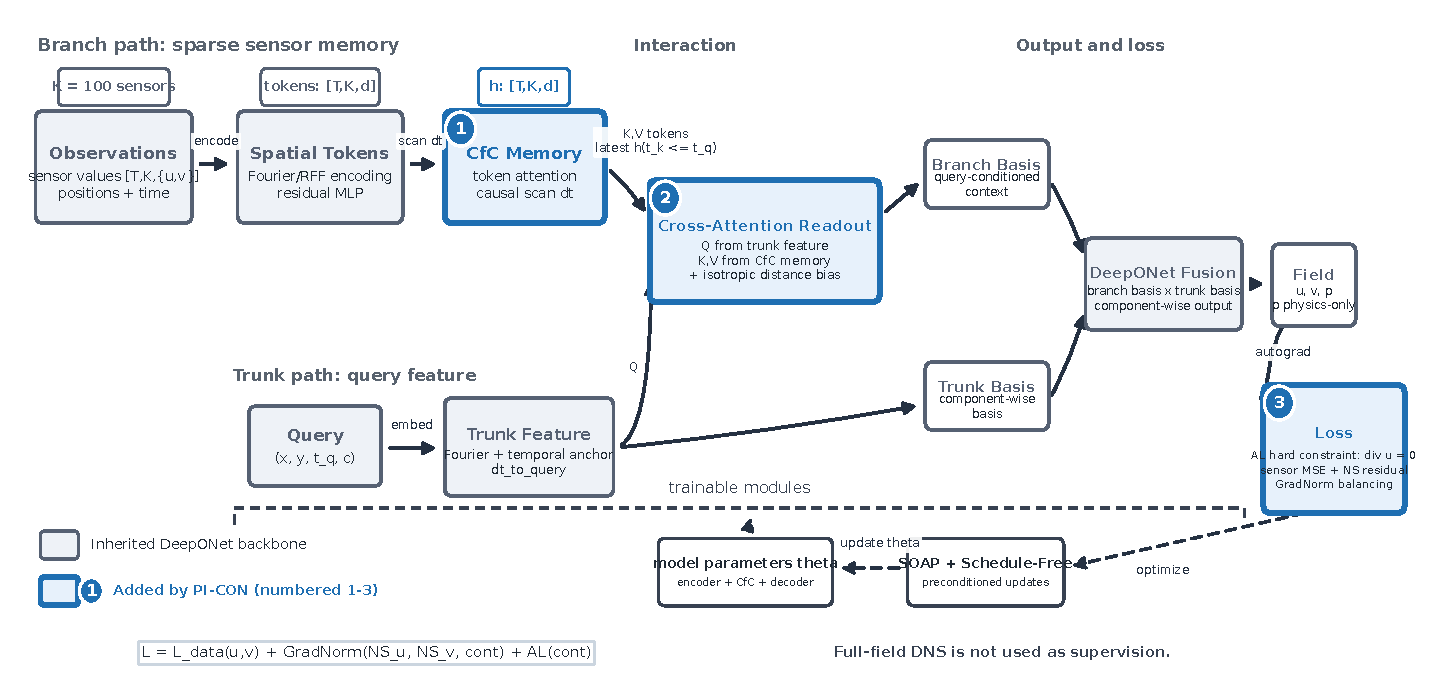
\includegraphics[width=1.3\linewidth]{figures/architecture/architecture.pdf}}
    \caption{PI-CON end-to-end signal flow. Grey boxes are the inherited DeepONet backbone; the three blue numbered boxes (1--3) are the additions in this work (1 CfC memory, 2 cross-attention readout, 3 the Augmented-Lagrangian continuity loss). Training uses sensor MSE and Navier--Stokes residuals only; no full-field DNS supervision.}
    \label{fig:architecture}
\end{figure}

\section{Engineering-Deployable Regime}
\label{sec:engineering_constraint}

Five conditions define the engineering deployment regime that every architectural and loss-design choice in this chapter must satisfy. They reflect the operational reality of in-situ flow reconstruction, where only sparse sensor measurements and the governing PDE are available rather than offline DNS post-processing.

\begin{enumerate}
    \item \textbf{Training supervision.} Only velocity components $(u,v)$ at sensor locations $\mathcal{S}$ supervise training. No DNS full-field signal enters, directly or through derived terms such as perceptual losses, spectral losses, VAE reconstructions, or latent priors.
    \item \textbf{Physics constraints.} The incompressible Navier--Stokes momentum and continuity residuals are enforced at random collocation points.
    \item \textbf{Data conditions.} DNS stands in for the experimentally inaccessible true flow in this controlled study, serving only to (a) extract sensor measurements at the LES-selected positions and (b) provide a reference field for offline a posteriori evaluation. \emph{The reference field never enters the training loss.}
    \item \textbf{Deployment assumption.} At deployment the model accesses only the same $K = 100$ fixed sensor positions and their time-stamped values; no DNS or full-field information is available.
    \item \textbf{Noise.} The main training runs use noise-free sensor measurements. Additive Gaussian noise robustness is a supporting engineering diagnostic; sensor-specific calibration errors lie outside the main objective.
\end{enumerate}

Figure~\ref{fig:pipeline} situates these conditions in the DNS-free deployment instance. Sensor placement is one of the sensing-configuration variables this work quantifies; here it takes the LES-derived, DNS-free form. The LES contributes sensor \emph{positions} only (a POD basis on which QR-pivoting selects the $K$ sites) and supplies no sensor values. The sensor \emph{values} are sampled at those positions from the DNS field that, in this controlled study, stands in for the experimentally inaccessible real-world flow. The label ``DNS-free'' therefore qualifies the placement step alone: siting the sensors needs no DNS, while the measurements read only $K$ point values and the full DNS field never enters training.

\begin{figure}[!htbp]
    \centering
    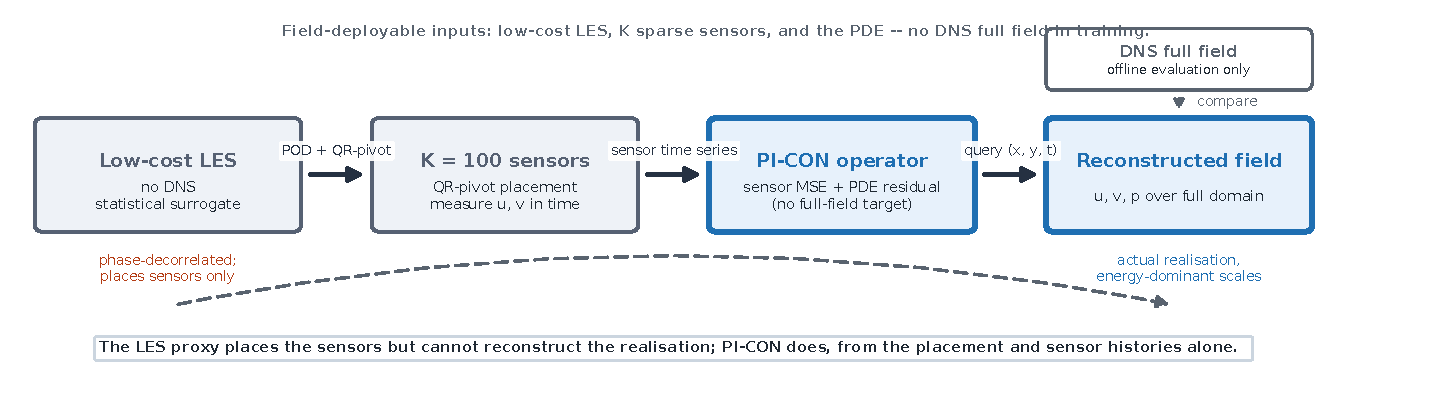
\includegraphics[width=\linewidth]{figures/architecture/pipeline.pdf}
    \caption{DNS-free deployment pipeline. The low-cost LES (green, top row) supplies only sensor \emph{positions} (POD + QR-pivot), not field values. Solid arrows: the deployable data path, where sensors read $u,v$ and PI-CON reconstructs a queryable $(u,v,p)$ field. Dashed: the full DNS field enters offline evaluation only, never training.}
    \label{fig:pipeline}
\end{figure}

\section{Modelling Assumptions}
\label{sec:assumptions}

The assumptions below are stated explicitly so that subsequent design choices and evaluation decisions remain amenable to local reasoning. The five supervision and deployment conditions of \S\ref{sec:engineering_constraint} are taken as given; the items below add further physical and numerical assumptions.

\begin{enumerate}
    \item \textbf{Governing equations.} The flow obeys the incompressible Navier--Stokes continuity and momentum equations (\S\ref{sec:problem_formulation}, equations~\eqref{eq:cont_main}--\eqref{eq:mom_main}). Compressibility, thermal effects, and non-Newtonian rheology are not modelled.
    \item \textbf{Geometry and boundary conditions.} The benchmark uses the periodic domain $\Omega = [0,1]^2$ with doubly periodic boundary conditions and no embedded obstacles. Non-periodic, wall-bounded, and obstacle-laden geometries are outside the present scope.
    \item \textbf{Known physical parameters.} The Reynolds number $Re$, kinematic viscosity $\nu = 1/Re$, forcing amplitude $A$, and forcing wavenumber $k_f$ are known a priori; parameter identification lies outside the inverse problem studied here.
    \item \textbf{Sensor placement and identity.} The sensor count $K$ and grid locations $\mathcal{S}$ are fixed before training and unchanged at inference, selected by QR-pivot on the POD basis (\S\ref{sec:sensor_placement}).
    \item \textbf{Channel availability.} Only the velocity components $(u, v)$ are measured at sensor positions. Vorticity $\omega$ serves as a diagnostic; pressure $p$ is a model-internal variable, not directly supervised.
    \item \textbf{Operator parameterization.} The reconstruction operator $\mathcal{G}_\theta$ is a single neural network returning $(u, v, p)$ at any query coordinate; no analytic decomposition or reduced-order basis is fixed outside the learnable parameters.
\end{enumerate}

\section{Governing Equations and Reconstruction Problem}
\label{sec:problem_formulation}

Consider an incompressible two-dimensional flow on the periodic domain $\Omega = [0,1]^2$ over the time interval $[0, T]$, governed by
\begin{subequations}
\label{eq:ns_main}
\begin{align}
    \nabla \cdot \mathbf{u} &= 0, \label{eq:cont_main}\\
    \frac{\partial \mathbf{u}}{\partial t} + (\mathbf{u}\cdot\nabla)\mathbf{u}
        &= -\nabla p + \nu\,\nabla^2 \mathbf{u} + \mathbf{f}, \label{eq:mom_main}
\end{align}
\end{subequations}
with $\mathbf{u}=(u,v)^T$, pressure $p$, and kinematic viscosity $\nu = 1/Re$. The Reynolds number used throughout is defined in \eqref{eq:re_def} as
\begin{equation}
    \label{eq:re_def}
    Re \;=\; \frac{U^* L^*}{\nu^*},
\end{equation}
where $L^* = 1$ m is the domain length scale, $U^* = 1$ m/s the reference velocity, and $\nu^*$ the kinematic viscosity. The main experiments use $Re = 10\,000$, giving $\nu^* = U^* L^* / Re = 10^{-4}$ m$^2$/s; the dimensionless form of \eqref{eq:ns_main} then has $\nu = 1/Re$. The Kolmogorov forcing is
\begin{equation}
    \label{eq:forcing}
    \mathbf{f}(\mathbf{x}) \;=\; \big(A\sin(2\pi k_f y),\; 0\big)^T,
\end{equation}
with $A = 0.1$, $k_f = 2$ in the main experiments at $Re=10\,000$.

\paragraph{Observation model.}
Measurements occupy $K$ fixed spatial locations $\mathcal{S} = \{\mathbf{x}_k\}_{k=1}^K$ at $N_t$ discrete time stamps $\{t_n\}_{n=1}^{N_t}$; each entry is $\mathbf{y}_{k,n} = (u(\mathbf{x}_k, t_n), v(\mathbf{x}_k, t_n))^T$. Per the engineering constraint of \S\ref{sec:engineering_constraint}, observed channels are restricted to $u$ and $v$; $\omega$ and $p$ are not measured.

\paragraph{Reconstruction target.}
The reconstruction operator is
\begin{equation}
    \label{eq:operator_def}
    \mathcal{G}_\theta : \;\big(\{\mathbf{y}_{k,n}\},\,\mathcal{S},\,\{t_n\}\big) \longmapsto (u, v, p)(\mathbf{x}, t)
\end{equation}
The operator in \eqref{eq:operator_def} is queriable at arbitrary $(\mathbf{x}, t) \in \Omega\times[0,T]$ and required to (i) match sensor observations on $\mathcal{S}\times\{t_n\}$ and (ii) satisfy the discrete residual of \eqref{eq:ns_main}. The parameters $\theta$ minimize the loss in \S\ref{sec:loss}.

\paragraph{Reconstruction target under an under-sampled snapshot.}
With $\mathbf{u}_t \in \mathbb{R}^N$ on the stored $256^2$ grid ($N = 65\,536$) and sensing operator $\mathbf{C}\in\{0,1\}^{K\times N}$, the snapshot equation $\mathbf{y}_t = \mathbf{C}\mathbf{u}_t$ is under-sampled: the compressed-sensing recovery threshold (\S\ref{sec:underdetermined}) sits roughly an order of magnitude above the $K=100$ budget, so exact pointwise recovery is not the goal. The achievable target is the energy-dominant low-wavenumber content: the architecture and physics constraints supply the structural prior that makes this band reconstructable, while the unresolved high-wavenumber modes lie beyond the sensor-count Nyquist scale $k_{\max}\approx\sqrt{K/\pi}$ (\S\ref{sec:underdetermined}).

\section{QR-pivot Sensor Placement}
\label{sec:sensor_placement}

Because $K \ll N$, sensor placement governs the achievable reconstruction error. The QRCP-on-POD-basis strategy of Manohar et al.~\cite{Manohar2018PNAS, Drmac2016SISC} selects $K$ row indices that minimize the conditioning of the sensing operator composed with the leading POD basis.

\paragraph{Snapshot matrix.}
$M$ snapshots $\{\mathbf{u}_{t_m}\}_{m=1}^M$ drawn uniformly from a DNS trajectory stack column-wise into $\mathbf{X}\in\mathbb{R}^{N\times M}$. The exposition treats $u$ as a single channel; the experiments use both measured velocity components to assemble the sensing basis.

\paragraph{POD basis.}
A truncated SVD,
\begin{equation*}
    \mathbf{X} \;=\; \mathbf{U}\,\boldsymbol{\Sigma}\,\mathbf{V}^T,
\end{equation*}
yields the dominant left singular vectors $\mathbf{U}_r = [\mathbf{u}_1\,|\,\cdots\,|\,\mathbf{u}_r]\in\mathbb{R}^{N\times r}$.

\paragraph{QRCP pivot selection.}
QR with column pivoting on $\mathbf{U}_r^T\in\mathbb{R}^{r\times N}$,
\begin{equation*}
    \mathbf{U}_r^T \,\mathbf{P} \;=\; \mathbf{Q}\,\mathbf{R},
\end{equation*}
yields a permutation $\mathbf{P}$ whose first $K$ columns identify the sensor grid locations $\mathcal{S}$. QRCP greedily picks columns that maximize the leading volume; the worst-case condition number of $\mathbf{C}\mathbf{U}_r$ obeys
\begin{equation*}
    \kappa(\mathbf{C}\mathbf{U}_r) \;\le\; \sqrt{1 + 4^K (N - K)}\,\frac{\sigma_{\max}(\mathbf{R}_{1:K,1:K})}{\sigma_{\min}(\mathbf{R}_{1:K,1:K})}.
\end{equation*}
In practice $\kappa$ from QRCP is much smaller than from random placement~\cite{Drmac2016SISC, Manohar2018PNAS}.

\paragraph{Concrete configuration.}
The main configuration sets $r$ automatically by a $99\%$ cumulative-variance threshold ($r\approx 60$), with $K=100$ and $M = 201$ DNS frames over $T=5$. The snapshot window spans one eddy turnover, so selected positions track dynamically informative regions.

\section{PI-CON Architecture}
\label{sec:architecture}

The architecture extends the contribution stated at the end of \S\ref{sec:research_questions}: vanilla DeepONet~\cite{Lu2021NMI} targets dense forward problems, and three of its building blocks must be replaced before it can address (O1)--(O3) under sparse sensing. Table~\ref{tab:deeponet_gaps} summarises the mapping; each gap is closed by one of the sub-networks introduced below.

\begin{table}[!htbp]
    \centering
    \caption{Three structural gaps of vanilla DeepONet under sparse-sensor reconstruction and the components introduced in this thesis to close them. All three additions build the reconstructor (O1); the right-hand column reports the role each plays.}
    \label{tab:deeponet_gaps}
    \small
    \setlength{\tabcolsep}{4pt}
    \begin{tabularx}{\textwidth}{>{\raggedright\arraybackslash}p{4.0cm}>{\raggedright\arraybackslash}p{4.4cm}>{\raggedright\arraybackslash}X}
    \toprule
    \textbf{Vanilla DeepONet gap} & \textbf{Addition in PI-CON} & \textbf{Role in the reconstructor (O1)} \\
    \midrule
    Branch ingests a fixed-grid snapshot; cannot handle an irregularly clocked sensor time signal. & Closed-form continuous-time (CfC) branch~\cite{Hasani2022CfC} (\S\ref{subsec:cfc_encoder}). & Reads the irregularly-clocked sensor time signal. \\
    Inner product is global; no spatial prior linking a query $(\mathbf{x},t)$ to the nearest sensors. & Cross-attention with isotropic distance bias~\cite{Vaswani2017Attention} (\S\ref{subsec:cross_attn}). & Sparse-to-dense field readout at any query. \\
    PDE residual is a soft penalty; continuity slips under sensor MSE alone. & Augmented-Lagrangian-style adaptive penalty on $\nabla\!\cdot\!\mathbf{u}$ (\S\ref{subsec:al_cont}). & Near-incompressible output field. \\
    \bottomrule
    \end{tabularx}
\end{table}

PI-CON comprises three sub-networks: (i) a sensor branch (spatial encoder, then a temporal CfC encoder, \S\ref{subsec:spatial_encoder}--\S\ref{subsec:cfc_encoder}); (ii) a trunk path (query encoder, \S\ref{subsec:trunk_path}); and (iii) a decoder (cross-attention, then DeepONet fusion, \S\ref{subsec:cross_attn}--\S\ref{subsec:operator_fusion}). The remaining components (learnable Fourier embedding~\cite{tancik2020fourierfeaturesletnetworks}, residual MLP encoder, and GradNorm auto-balancing~\cite{Chen2018ICML}) are standard and are introduced briefly where they appear.

\subsection{Sensor Branch: Spatial Set Encoder}
\label{subsec:spatial_encoder}

\paragraph{Motivation.}
The spatial set encoder converts the $K$ simultaneous point measurements into per-sensor feature vectors that retain each sensor's location, so the decoder can later weight each sensor by its proximity to a query point: the discrete analogue of attaching a basis function to every measurement station.

\paragraph{Inputs.}
At a single time stamp, sensor observations are $\mathbf{s} \in \mathbb{R}^{K\times 2}$ (already normalized) at locations $\{\mathbf{x}_k\}_{k=1}^K \in \Omega$.

\paragraph{Position encoding (Learnable Fourier embedding).}
The periodic domain calls for a learnable Fourier embedding. Each sensor location $\mathbf{x}_k = (x, y)$ is first periodicized as
\begin{equation*}
    \mathbf{e}(\mathbf{x}_k) \;=\; \big[\sin\!\tfrac{2\pi x}{L},\,\cos\!\tfrac{2\pi x}{L},\,\sin\!\tfrac{2\pi y}{L},\,\cos\!\tfrac{2\pi y}{L}\big]^T \;\in\;\mathbb{R}^4,
\end{equation*}
then linearly projected into the Fourier feature space:
\begin{equation}
    \label{eq:learnable_fourier}
    \gamma(\mathbf{x}_k) \;=\; \big[\cos(\mathbf{W}\,\mathbf{e}(\mathbf{x}_k)),\;\sin(\mathbf{W}\,\mathbf{e}(\mathbf{x}_k))\big]^T \;\in\;\mathbb{R}^{d_{\text{emb}}},
\end{equation}
where $\mathbf{W}\in\mathbb{R}^{(d_{\text{emb}}/2)\times 4}$ is initialized with $\mathcal{N}(0, \sigma^2)$ entries ($\sigma=2.0$) and learned jointly with the rest of the network ($d_{\text{emb}} = 128$). The trainable projection in \eqref{eq:learnable_fourier} adapts the frequency mixture and mitigates spectral bias~\cite{Rahaman2019Spectral}, unlike fixed-$\sigma$ Fourier features~\cite{tancik2020fourierfeaturesletnetworks}.

\paragraph{Token MLP and residual encoding.}
Concatenating position encoding and sensor measurement gives
\begin{equation*}
    \mathbf{f}_k \;=\; [\gamma(\mathbf{x}_k);\,\mathbf{s}_k] \;\in\;\mathbb{R}^{d_{\text{emb}}+2},
\end{equation*}
projected to width $d_{\text{model}} = 256$ by
\begin{equation*}
    \mathbf{e}_k^{(0)} \;=\; \mathrm{Linear}\!\big(\mathrm{SiLU}(\mathrm{Linear}(\mathrm{LayerNorm}(\mathbf{f}_k)))\big).
\end{equation*}
The token then passes through $L_s = 1$ residual MLP block:
\begin{equation}
    \label{eq:residual_block}
    \mathbf{e}_k^{(\ell)} \;=\; \mathbf{e}_k^{(\ell-1)} + \mathrm{MLP}\!\big(\mathrm{LayerNorm}(\mathbf{e}_k^{(\ell-1)})\big),\quad \ell=1,\ldots,L_s.
\end{equation}
The residual update in \eqref{eq:residual_block} is followed by an output projection (LayerNorm $\to$ Linear$_{d\to 2d}$ $\to$ SiLU $\to$ Linear$_{2d\to d}$) that yields the spatial token $\mathbf{z}_k \in \mathbb{R}^{d_{\text{model}}}$.

\paragraph{Design rationale.}
Tokens stay per-sensor rather than pooled, because the downstream cross-attention (\S\ref{subsec:cross_attn}) requires a per-query attention distribution over individual sensors: unrecoverable once pooled.

\subsection{Token Self-Attention}
\label{subsec:token_attn}

Neighbouring sensors sample correlated flow structures (a single vortex may straddle several stations), so each sensor's representation is sharpened by letting it attend to the others before the temporal branch evolves it. Before each CfC scan, sensor tokens pass through a token self-attention block~\cite{Vaswani2017Attention} (multi-head, $h=4$, $L_a=2$ layers):
\begin{equation}
    \label{eq:self_attn}
    \hat{\mathbf{Z}} \;=\; \mathbf{Z} + \mathrm{MultiheadAttn}(\mathrm{LayerNorm}(\mathbf{Z})),
    \quad \mathbf{Z}' \;=\; \hat{\mathbf{Z}} + \mathrm{FFN}(\mathrm{LayerNorm}(\hat{\mathbf{Z}})),
\end{equation}
with $\mathbf{Z} = [\mathbf{z}_1\,|\,\cdots\,|\,\mathbf{z}_K]^T \in\mathbb{R}^{K\times d_{\text{model}}}$ and FFN realised as Linear$_{d\to 2d}$ $\to$ SiLU $\to$ Linear$_{2d\to d}$. The update in \eqref{eq:self_attn} lets sensors exchange spatial information (e.g.\ upstream--downstream) while preserving the token identity required by the downstream causal cross-attention.

\subsection{Closing the Time-Signal Gap: CfC Continuous-Time Branch}
\label{subsec:cfc_encoder}

\paragraph{Motivation.}
The CfC branch compresses each sensor's time history into a compact state that tracks recent dynamics while tolerating irregular sampling intervals. Sensor time series $\mathbf{s}_k(t_n)$, $n=1,\ldots,N_t$, arrive on irregular clocks: packets drop, groups report on different cadences, and inference must accept whatever timestamps arrive. Discrete RNNs (GRU, LSTM) cannot absorb such irregular sampling; Neural ODE~\cite{Chen2018NODE} offers a continuous-time view at the cost of an ODE solver per step. CfC~\cite{Hasani2022CfC} provides a closed-form solution to LTC dynamics~\cite{Hasani2021LTC} at per-step cost comparable to a discrete RNN, and is therefore adopted here.

This choice also keeps training tractable on the stiff high-$Re$ case: stabilized MLP-based PINNs reach this regime by splitting the time domain into sequential windows and fitting one network per window (PirateNet~\cite{Wang2024JMLR} uses ten intervals, each initialized from the previous window's solution, and the second-order-optimized variant~\cite{wang2025gradientalignmentpinns} relies on time-marching and curriculum training), so their cost scales with the number of windows.

The CfC branch instead encodes the whole sensor time series in a single continuous-time pass, with a closed-form update that its authors report to train and run at least two orders of magnitude faster than ODE-based continuous-time models~\cite{Hasani2022CfC}; the liquid-network family it belongs to is also compact and noise-robust~\cite{Lechner2020NCP}. A CfC encoder is therefore preferred over a vanilla DeepONet branch or an MLP-PINN backbone for the sensor stream.

\paragraph{CfC cell.}
With cell input $\mathbf{c}_t \in \mathbb{R}^{d_{\text{in}}}$, hidden state $\mathbf{h}_t \in \mathbb{R}^{d_{\text{model}}}$, and time gap $\Delta t = t_n - t_{n-1}$, the CfC update is
\begin{subequations}
\label{eq:cfc}
\begin{align}
    f_1(\mathbf{c},\mathbf{h}) &= \tanh(\mathbf{W}_1[\mathbf{c};\mathbf{h}] + \mathbf{b}_1),\\
    f_2(\mathbf{c},\mathbf{h}) &= \tanh(\mathbf{W}_2[\mathbf{c};\mathbf{h}] + \mathbf{b}_2),\\
    \boldsymbol{\sigma}(\mathbf{c},\mathbf{h};\Delta t) &= \mathrm{sigmoid}\!\big(-\boldsymbol{\tau}_a\,\Delta t + \mathbf{t}_b([\mathbf{c};\mathbf{h}])\big),\\
    \mathbf{h}_{t+\Delta t} &= \boldsymbol{\sigma} \odot f_1 + (1-\boldsymbol{\sigma}) \odot f_2,
\end{align}
\end{subequations}
where $\mathbf{c}$ denotes the cell input (distinct from the spatial coordinate $\mathbf{x}$ used elsewhere) and $\mathbf{h}$ the recurrent hidden state. In the CfC update \eqref{eq:cfc}, $\boldsymbol{\sigma}$ blends a fast-response candidate state $f_1$ with a slow-relaxation candidate $f_2$. Because the time gap $\Delta t$ enters $\boldsymbol{\sigma}$ directly, a longer silence between sensor samples shifts the blend toward the relaxed state; this is how the cell absorbs irregular sampling instead of assuming a fixed clock. The element-wise time constants $\boldsymbol{\tau}_a = \exp(\boldsymbol{\tau}_a^{(\theta)})$ come from a learnable log-space parameter $\boldsymbol{\tau}_a^{(\theta)}\in\mathbb{R}^{d_{\text{model}}}$. It is initialized as $\mathrm{linspace}(\log\tau_{\min}, \log\tau_{\max}, d_{\text{model}})$ with $[\log\tau_{\min}, \log\tau_{\max}] = [-1, 1]$, so that $\tau \in [e^{-1}, e^{1}] \approx [0.37, 2.72]$; the exponential parametrization enforces positivity. The term $\mathbf{t}_b(\cdot) = \mathbf{W}_t[\mathbf{c};\mathbf{h}] + \mathbf{b}_t$ is a learnable input-dependent affine time shift.

\paragraph{Multi-layer multi-time scan.}
Let $L_t$ denote the number of CfC layers ($L_t = 1$ in the main experiment). Each layer performs (i) token self-attention vectorized over time, (ii) addition of a Reynolds-number bias $\mathbf{r}_e = \mathrm{Linear}(Re_{\text{norm}}) \in \mathbb{R}^{d_{\text{model}}}$ that lets the network adapt its time scales across $Re$, and (iii) a CfC forward scan. The CfC cell input at sensor $k$, time index $n$ is $\mathbf{c}_{k,n} = \mathbf{z}'_k + \mathbf{r}_e \in \mathbb{R}^{d_{\text{model}}}$ ($d_{\text{in}} = d_{\text{model}}$), the self-attention-refined spatial token tiled across $N_t$ time steps and shifted by the $Re$ bias:
\begin{equation*}
    \mathbf{h}_{k,n} \;=\; \mathrm{CfCCell}(\mathbf{c}_{k,n},\,\mathbf{h}_{k,n-1};\,\Delta t_n),
    \quad n=1,\ldots,N_t,\;k=1,\ldots,K,
\end{equation*}
with $\Delta t_n = t_n - t_{n-1}$. The output is the branch token-state tensor $\mathbf{H}\in\mathbb{R}^{N_t\times K\times d_{\text{model}}}$.

\paragraph{Bidirectional option (smoothing mode).}
An optional backward scan from $t_{N_t}$ to $t_1$ produces $\mathbf{h}^{(B)}_{k,n}$, added to the forward state $\mathbf{h}^{(F)}_{k,n}$. This mode applies to offline batch reconstruction (smoothing); deployment-oriented filtering uses the forward scan alone.

\subsection{Trunk Path: Query Encoding}
\label{subsec:trunk_path}

\paragraph{Query input.}
A query is $(x, y, t, c)$ with $c\in\{0, 1, 2\}$ indexing the output channel ($0\!=\!u$, $1\!=\!v$, $2\!=\!p$).

\paragraph{Spatial encoding.}
The Learnable Fourier embedding of the sensor branch (separate but identically structured weights) yields $\gamma(\mathbf{x}_q) \in \mathbb{R}^{d_{\text{emb}}}$.

\paragraph{Temporal encoding.}
The temporal feature combines an absolute phase anchor with a causal time gap. The phase anchor
\begin{equation*}
    \boldsymbol{\phi}(t) \;=\; \big[\sin\!\tfrac{2\pi n t}{T_{\text{total}}},\,\cos\!\tfrac{2\pi n t}{T_{\text{total}}}\big]_{n=1}^{N_h}\;\in\;\mathbb{R}^{2N_h},
\end{equation*}
with $N_h = 2$ and $T_{\text{total}} = 5$, supplies an absolute time reference independent of any relative offset. Given the latest sensor timestamp $t_{n^*(q)} \le t_q$, the causal time gap $\Delta t_q = t_q - t_{n^*(q)}$ projects to dimension $d_t = 16$ via $\mathbf{e}_t = \mathrm{Linear}(\Delta t_q)$.

\paragraph{Channel embedding.}
$\mathbf{e}_c = \mathrm{Embedding}(c) \in \mathbb{R}^8$ for $c\in\{0,1,2\}$.

\paragraph{Trunk feature.}
The concatenated input feeds a trunk MLP:
\begin{equation*}
    \mathbf{q}_{\text{trunk}} \;=\; \mathrm{TrunkMLP}([\gamma(\mathbf{x}_q);\,\boldsymbol{\phi}(t);\,\mathbf{e}_t;\,\mathbf{e}_c]) \;\in\;\mathbb{R}^{d_{\text{hidden}}},
\end{equation*}
an initial SiLU projection followed by $L_q = 1$ residual MLP blocks.

\subsection{Closing the Sparse-to-Dense Gap: Cross-Attention with Isotropic Distance Bias}
\label{subsec:cross_attn}

For each reconstruction point $(\mathbf{x}, t)$, the cross-attention readout learns how strongly every one of the $K=100$ sensors relates to that query. This turns query--sensor distance into a relevance weight, so the field value is built from location-specific sensor evidence rather than from a pooled comparison against the whole sensor set. This is the sparse-to-dense fusion required by the engineering setting: a continuous query must aggregate information from $K=100$ irregularly placed sensor tokens, with weights adapted to spatial proximity and physical similarity. Originating in the Transformer~\cite{Vaswani2017Attention} and extended by Perceiver~\cite{Jaegle2021Perceiver} to variable-size inputs, cross-attention natively handles irregular sensor sets. Two modifications adapt it to fluid reconstruction: an isotropic relative-position bias and a causal lookup over sensor time.

\paragraph{Causal lookup.}
Given query time $t_q$ and the strictly increasing sensor clock $\{t_n\}_{n=1}^{N_t}$, binary search returns the most recent timestamp not exceeding $t_q$:
\begin{equation}
    \label{eq:searchsorted}
    n^*(q) \;=\; \mathrm{clamp}\!\big(\mathrm{searchsorted}(\{t_n\},\,t_q,\,\mathrm{right=True}) - 1,\;0,\;N_t-1\big),
\end{equation}
the decoder then reads $\mathbf{H}_q = \mathbf{H}[n^*(q),\,:,\,:] \in \mathbb{R}^{K\times d_{\text{model}}}$. The lookup in \eqref{eq:searchsorted} enforces filtering causality: the query accesses sensor information only up to time $t_q$.

\paragraph{Isotropic relative-position bias.}
The cross-attention does \emph{not} use a directional relative position $(r_x, r_y)$. The isotropic distance kernel is a deliberate modelling simplification: although the Kolmogorov forcing $f_x = A\sin(2\pi k_f y)$ makes the flow statistically anisotropic, a directional bias would implicitly encode the non-uniform $x$-distribution of the QR-pivot sensors as a spurious directional attention term, whereas the isotropic norm $|\mathbf{r}|$ admits no such mechanism.

For query position $\mathbf{x}_q$ and sensor positions $\{\mathbf{x}_k\}$, the relative position $\mathbf{r}_{qk} = \mathbf{x}_q - \mathbf{x}_k$ folds onto the torus by
\begin{equation*}
    \mathbf{r}_{qk} \;\leftarrow\; \mathbf{r}_{qk} - L\cdot\mathrm{round}(\mathbf{r}_{qk}/L),
\end{equation*}
and a smooth norm follows:
\begin{equation}
    \label{eq:smooth_norm}
    r_{qk} \;=\; \sqrt{\Vert\mathbf{r}_{qk}\Vert_2^2 + \varepsilon},\quad \varepsilon = 10^{-8}.
\end{equation}
The $\varepsilon$ in \eqref{eq:smooth_norm} is required: when a collocation point coincides with a sensor ($\mathbf{r}_{qk}=\mathbf{0}$), the second-order autograd of $\Vert\mathbf{r}\Vert_2$, $(\Vert r\Vert^2 I - rr^T)/\Vert r\Vert^3$, evaluates to $0/0$ and yields a NaN inside the NS residual (observed on a non-periodic-domain test case where sensors and collocation points overlap with high probability). The smooth norm has a finite second derivative $\varepsilon^{-1/2}$ at $r = 0$, eliminating the NaN source.

The scalar distance maps to a scalar attention bias:
\begin{equation*}
    b_{qk} \;=\; \mathrm{MLP}_{\text{relpos}}(\mathrm{LayerNorm}(r_{qk})) \;\in\;\mathbb{R},
\end{equation*}
where $\mathrm{MLP}_{\text{relpos}}$ is LayerNorm $\to$ Linear$_{1\to d}$ $\to$ SiLU $\to$ Linear$_{d\to 1}$.

\paragraph{Cross-attention.}
Queries come from the trunk feature; keys and values from the branch token states. Let $\mathrm{TokenProj}:\mathbb{R}^{d_{\text{model}}}\!\to\!\mathbb{R}^{d_{\text{hidden}}}$ denote a single linear layer (with LayerNorm) applied per branch token before key/value projection:
\begin{align}
    \mathbf{Q}_q &= \mathbf{W}_Q\,\mathrm{LayerNorm}(\mathbf{q}_{\text{trunk}}),\\
    \mathbf{K}_k &= \mathbf{W}_K\,\mathrm{TokenProj}(\mathbf{H}_q[k]),\quad
    \mathbf{V}_k = \mathbf{W}_V\,\mathrm{TokenProj}(\mathbf{H}_q[k]).
\end{align}
The attention weights are
\begin{equation}
    \label{eq:attention}
    A_{qk} \;=\; \mathrm{softmax}_k\!\Big(\frac{\mathbf{Q}_q^T\mathbf{K}_k}{\sqrt{d_{\text{hidden}}}} + b_{qk}\Big),
\end{equation}
and the branch context is
\begin{equation*}
    \mathbf{c}_{\text{branch}}(q) \;=\; \sum_{k=1}^K A_{qk}\,\mathbf{V}_k + \mathrm{MLP}_{\text{ctx}}\!\Big(\sum_{k=1}^K A_{qk}\,\mathbf{V}_k\Big),
\end{equation*}
where $\mathrm{MLP}_{\text{ctx}}$ is a residual refinement of the attention output. Equation~\eqref{eq:attention} is the only place where the isotropic relative-position bias changes the attention logits.

\subsection{DeepONet-style Operator Fusion}
\label{subsec:operator_fusion}

\paragraph{Branch and trunk basis vectors.}
Each context vector projects onto a rank-$R$ basis ($R = 256$), sliced by channel $c$:
\begin{align}
    \boldsymbol{\Psi}^{\text{trunk}} &= \mathrm{Linear}_{d_{\text{hidden}}\to 3R}(\mathbf{q}_{\text{trunk}}) \in\mathbb{R}^{3\times R},\\
    \boldsymbol{\Psi}^{\text{branch}} &= \mathrm{Linear}_{d_{\text{hidden}}\to 3R}(\mathbf{c}_{\text{branch}}) \in\mathbb{R}^{3\times R}.
\end{align}
The channel-$c$ row yields $\boldsymbol{\psi}^{\text{trunk}}_c, \boldsymbol{\psi}^{\text{branch}}_c \in \mathbb{R}^R$.

\paragraph{Tensor-product fusion.}
The fusion mirrors a modal (POD-like) expansion: the trunk vector $\boldsymbol{\psi}^{\text{trunk}}_c$ supplies $R$ query-evaluated mode shapes, the branch vector $\boldsymbol{\psi}^{\text{branch}}_c$ the sensor-derived modal coefficients, and their inner product reconstructs the channel value the way $\sum_r a_r\phi_r(\mathbf{x})$ rebuilds a field from a POD basis. The DeepONet output is the element-wise inner product of the two basis vectors:
\begin{equation}
    \label{eq:fusion}
    \widetilde{u}_c(\mathbf{x}_q,t_q) \;=\; \tau_{\text{out}} \cdot \big(\boldsymbol{\psi}^{\text{trunk}}_c \odot \boldsymbol{\psi}^{\text{branch}}_c\big) \cdot \mathbf{1}
    \;=\; \tau_{\text{out}} \cdot \sum_{r=1}^R \psi^{\text{trunk}}_{c,r}\,\psi^{\text{branch}}_{c,r},
\end{equation}
with learnable scalar gain $\tau_{\text{out}} = \exp(\log\tau_{\text{out}}^{(\theta)})$ initialized at $1/\sqrt{R}$ (this DeepONet temperature is distinct from the CfC time-constant vector $\boldsymbol{\tau}_a$ of \S\ref{subsec:cfc_encoder}). A per-channel affine map then produces the prediction:
\begin{equation}
    \label{eq:output_head}
    u_c \;=\; \gamma_c\,\widetilde{u}_c + \beta_c,
\end{equation}
with learnable scalars $\gamma_c, \beta_c$ and $\gamma_c$ initialized to $g_{\text{out}} = 1$. The affine head in \eqref{eq:output_head} restores the channel-wise scale after the shared DeepONet basis expansion.

\paragraph{Inductive bias.}
Equation~\eqref{eq:fusion} expands the output as a sum of $R$ basis functions, each the product of a query-dependent trunk basis and a sensor-content-dependent branch basis. The factorization decouples spatial query from sensor encoding: once trained, the operator may be queried at any continuous coordinate $(\mathbf{x}, t)\in\Omega\times[0,T]$ without retraining or re-meshing, meeting the engineering need for on-demand reconstruction at arbitrary probe locations. The DeepONet universal-approximation theorem~\cite{Lu2021NMI} guarantees that any continuous operator can be approximated to arbitrary accuracy as $R \to \infty$; at finite $R$ the rank bounds effective capacity. The main experiment sets $R = d_{\text{model}} = 256$.

\section{Loss Function}
\label{sec:loss}

Per \S\ref{sec:engineering_constraint}, the training objective uses only sensor measurements at $\mathcal{S}\times\{t_n\}$ and the incompressible Navier--Stokes residual at random collocation points; no DNS full-field signal enters the loss. The objective is a weighted sum with weights dynamically adjusted by GradNorm auto-balancing~\cite{Chen2018ICML}:
\begin{equation}
    \label{eq:total_loss}
    \mathcal{L}(\theta) \;=\; w_{\text{data}}\,\mathcal{L}_{\text{data}}
                  + w_{\text{NS},u}\,\mathcal{L}_{\text{NS},u}
                  + w_{\text{NS},v}\,\mathcal{L}_{\text{NS},v}
                  + w_{\text{cont}}\,\mathcal{L}_{\text{cont}}
                  + \mathcal{L}_{\text{AL}},
\end{equation}
where $\mathcal{L}_{\text{AL}}$ is the Augmented-Lagrangian-style continuity penalty (\S\ref{subsec:al_cont}; $\mathcal{L}_{\text{AL}}=0$ when AL is disabled), added to the objective outside the GradNorm weighting. The four GradNorm-managed tasks in \eqref{eq:total_loss} are $\{\mathcal{L}_{\text{data}},\, \mathcal{L}_{\text{NS},u},\, \mathcal{L}_{\text{NS},v},\, \mathcal{L}_{\text{cont}}\}$; in the main configuration continuity enters both as this GradNorm-balanced soft term and through the adaptive AL penalty acting on the same residual.

\subsection{Sensor Data Loss with Initial-Condition Emphasis}

For $N$ randomly drawn observation triples $(\mathbf{x}_k, t_n, c)$ with $c \in \{0, 1\}$ ($u, v$):
\begin{equation}
    \label{eq:data_loss}
    \mathcal{L}_{\text{data}} \;=\; \frac{1}{N}\sum_{i=1}^{N} w_i\,\Big(\hat{u}_{c_i}(\mathbf{x}_i,t_i;\theta) - u^{\text{obs}}_{c_i}(\mathbf{x}_i,t_i)\Big)^2,
\end{equation}
where the data loss in \eqref{eq:data_loss} uses the IC weight
\begin{equation}
    w_i \;=\; \begin{cases} w_{\text{early}} & t_i \le t_{\text{early}},\\ 1 & t_i > t_{\text{early}}.\end{cases}
\end{equation}
The main experiment sets $t_{\text{early}} = 0.05$ and $w_{\text{early}} = 10$. The emphasis targets the initial-condition reconstruction window, which carries the highest per-step uncertainty in chaotic flow.

\subsection{NS Momentum Residuals}

Automatic differentiation of the network output yields the PDE residuals:
\begin{align}
    \label{eq:res_u}
    \mathcal{R}_u &= \frac{\partial u}{\partial t} + u\frac{\partial u}{\partial x} + v\frac{\partial u}{\partial y} + \frac{\partial p}{\partial x} - \nu\Big(\frac{\partial^2 u}{\partial x^2}+\frac{\partial^2 u}{\partial y^2}\Big) - f_x,\\
    \label{eq:res_v}
    \mathcal{R}_v &= \frac{\partial v}{\partial t} + u\frac{\partial v}{\partial x} + v\frac{\partial v}{\partial y} + \frac{\partial p}{\partial y} - \nu\Big(\frac{\partial^2 v}{\partial x^2}+\frac{\partial^2 v}{\partial y^2}\Big),
\end{align}
with $f_x = A\sin(2\pi k_f y)$. The two residuals in \eqref{eq:res_u}--\eqref{eq:res_v} share the same collocation batch, and the smooth norm \eqref{eq:smooth_norm} guarantees that second-order autograd produces no NaN at sensor-coincident points.

The momentum residual losses are
\begin{equation*}
    \mathcal{L}_{\text{NS},u} = \frac{1}{N_p}\sum_{j=1}^{N_p}\mathcal{R}_u^2(\mathbf{x}_j, t_j),\quad
    \mathcal{L}_{\text{NS},v} = \frac{1}{N_p}\sum_{j=1}^{N_p}\mathcal{R}_v^2(\mathbf{x}_j, t_j),
\end{equation*}
with $N_p = 1024$ random collocation points per step and $t_j \sim \mathcal{U}(0, t_{\max}(\text{step}))$, where $t_{\max}$ follows the time-marching curriculum (\S\ref{sec:training_protocol}).

\subsection{Continuity Residual}
\label{subsec:continuity}

\begin{equation}
    \label{eq:cont_res}
    \mathcal{R}_c \;=\; \frac{\partial u}{\partial x} + \frac{\partial v}{\partial y},\quad \mathcal{L}_{\text{cont}} = \frac{1}{N_p}\sum_{j=1}^{N_p}\mathcal{R}_c^2(\mathbf{x}_j,t_j).
\end{equation}

\subsection{Closing the Physics-Consistency Gap: Augmented Lagrangian on Continuity}
\label{subsec:al_cont}

The Augmented-Lagrangian-style (AL) term adds an adaptive penalty that progressively tightens the continuity constraint rather than merely discouraging its violation at a fixed weight. Incompressibility matters for engineering use: a field with large $\nabla\!\cdot\!\mathbf{u}$ is unphysical regardless of pointwise accuracy. GradNorm balances gradient magnitudes across the four tasks but imposes no floor on the continuity residual; an AL-style penalty~\cite{NocedalWright2006} augments the same mean-squared continuity residual $C \equiv \mathcal{L}_{\text{cont}}$ with a dual variable $\lambda$ that grows while the residual stays above zero:
\begin{equation}
    \label{eq:al_loss}
    \mathcal{L}_{\text{AL}} \;=\; \lambda\,C \;+\; \frac{\rho}{2}\,C^2,
\end{equation}
where $C = \mathcal{L}_{\text{cont}} = \frac{1}{N_p}\sum_{j=1}^{N_p}\mathcal{R}_c^2(\mathbf{x}_j, t_j)$ is the non-negative mean-squared divergence already entering the soft term, evaluated on the same collocation points, and $\rho > 0$ is the penalty strength. The penalty in \eqref{eq:al_loss} uses the squared residual rather than a signed mean, so it admits no sign cancellation: the constraint quantity is bounded below by zero. Every $\Delta_{\text{AL}} = 100$ steps the dual variable updates from an exponential moving average of $C$:
\begin{equation}
    \label{eq:al_update}
    \tilde{C}_{\text{ema}} \;\leftarrow\; (1-\beta)\,\tilde{C}_{\text{ema}} \;+\; \beta\,C,\qquad
    \lambda \;\leftarrow\; \mathrm{clip}\!\Big(\lambda + \rho\,\tilde{C}_{\text{ema}},\;0,\;\Lambda_{\max}\Big),
\end{equation}
with $\beta=0.5$ and clip ceiling $\Lambda_{\max}=10$. Because $C \ge 0$, the update in \eqref{eq:al_update} drives $\lambda$ monotonically upward, with $\Lambda_{\max}$ bounding it from above; the multiplier settles as the residual falls rather than by reaching that bound. The scheme thus acts as an accumulated-multiplier penalty schedule that steadily raises the effective continuity weight, rather than a textbook equality-constraint Lagrangian (whose multiplier would change sign). The lower clip at zero keeps $\lambda$ physically non-negative.

When AL is on, $\mathcal{L}_{\text{AL}}$ is added to the objective \eqref{eq:total_loss}, so GradNorm still manages the four-task weights while AL applies added pressure through $\lambda$. The penalty strength $\rho$ is a tuneable hyperparameter.

\subsection{GradNorm Auto-balancing}
\label{subsec:gradnorm}

The four loss terms differ markedly in scale across training, so static weighting cannot cope with the resulting dynamics. Equalizing the per-task gradient magnitudes automates the weight tuning a practitioner would otherwise perform by hand, preventing large momentum-residual gradients from swamping the much smaller continuity gradient (or the reverse). A custom GradNorm scheme adapted from~\cite{Chen2018ICML, Sener2018MOO} is used. Every $\Delta_g = 1\,000$ steps, per-task gradient norms are computed against a reference parameter $\theta_r$ (the trunk output linear-layer weight and bias); equalization-target weights are then derived, normalized against $w_{\text{data}}^{\text{target}}$ to suppress absolute scale drift, and EMA-smoothed:
\begin{align}
    G_i &= \Vert \nabla_{\theta_r} \mathcal{L}_i \Vert_2,
        \quad i\in\{\text{data},\,\text{NS-u},\,\text{NS-v},\,\text{cont}\},\\
    w_i^{\text{target}} &= \frac{\overline{G}}{G_i + 10^{-5}\overline{G}},
        \qquad \overline{G} = \tfrac{1}{4}\sum_i G_i,\\
    w_i^{\text{norm}} &= w_i^{\text{target}} / w_{\text{data}}^{\text{target}},\\
    w_i^{(\text{new})} &= m\,w_i^{(\text{old})} + (1-m)\,w_i^{\text{norm}},\quad m = 0.9,
\end{align}
where $w_i^{(\text{new})}$ may be clamped from below by a non-negative floor. In the main experiments dynamic balancing alone gave stability over $20\,000$ training steps.

\paragraph{Differences from the original GradNorm.}
Chen et al.~\cite{Chen2018ICML} use a relative training rate to compute target weights. The present variant directly equalizes gradient norms against a reference parameter, normalizes by $w_{\text{data}}^{\text{target}}$ to suppress absolute scale drift, and EMA-smooths to damp oscillations. Initial weights $[w_{\text{data}}, w_{\text{NS},u}, w_{\text{NS},v}, w_{\text{cont}}] = [1, 0.057, 0.057, 0.01]$ start the momentum terms at $5.7\%$ and continuity at $1\%$ of the data weight.

\section{Optimization Stack}
\label{sec:optimization}

The coupled sensor-MSE and PDE-residual objective is stiff and ill-conditioned: the second-derivative (Laplacian) physics terms and the data term curve differently, so a quasi-second-order optimizer that rescales the gradient by an approximate Hessian converges where plain first-order Adam stalls. The components below implement this idea.

\paragraph{SOAP optimizer.}
SOAP~\cite{Vyas2024SOAP}, a quasi-second-order method that approximates the Hessian via Shampoo-style factorization and applies Adam in the preconditioner eigenbasis, is adopted here following its use for second-order PINN optimization~\cite{wang2025gradientalignmentpinns}; it gives better stability than vanilla Adam in the multi-task PINN setting. Main settings: Adam-style betas $(0.9,0.999)$, frequent preconditioner updates, initial learning rate $10^{-3}$.

\paragraph{Schedule-Free wrapper.}
SOAP is wrapped in a Schedule-Free~\cite{ScheduleFree2024} layer that performs Polyak--Ruppert averaging in place of explicit learning-rate decay.

\paragraph{Learning-rate schedule.}
A staircase decay applies: linear warmup over $2\,000$ steps to $\text{lr} = 10^{-3}$, then multiplicative decay $\gamma_{\text{decay}} = 0.9$ every $2\,000$ steps. ($\gamma_{\text{decay}}$ avoids collision with the AL dual variable $\lambda$ of \S\ref{subsec:al_cont}.) Gradient clipping is enforced at $\Vert g\Vert_\infty \le 1.0$.

\section{Training Protocol}
\label{sec:training_protocol}

\paragraph{Time-marching curriculum.}
Following the causality principle of Wang 2022~\cite{wang2022respectingcausality}, collocation and query times are capped at
\begin{equation*}
    t_{\max}(s) \;=\; t_{\text{start}} + (T - t_{\text{start}})\cdot\min\!\Big(\frac{\max(0,\,s-s_w)}{\Delta s},\;1\Big),
\end{equation*}
with $t_{\text{start}}=0.5$, no fixed hold ($s_w = 0$), and a linear ramp of $\Delta s = 2\,000$ steps. The horizon expands from $t \le 0.5$ at the first step to the full $t \le T = 5$ by step $2\,000$, then stays at $T$, blocking early-time chaotic error from contaminating the global loss.

\paragraph{Sensor temporal trimming.}
While $t_{\max}(s) < T$, the sensor branch encoder reads only $t \le t_{\max}(s)$, keeping the CfC branch consistent with the query-side time-marching restriction.

\paragraph{Physics warmup / ramp.}
GradNorm balances physics weights dynamically; no additional warmup ramp is imposed. Random collocation drives the physics residuals throughout training.

\paragraph{Training loop.}
Algorithm~\ref{alg:training} summarizes the full procedure.

\begin{algorithm}[H]
\SetAlgoLined
\small
\caption{PI-CON training loop (filtering mode)}
\label{alg:training}
\KwIn{Sensor data $\mathbf{D}=\{\mathbf{y}_{k,n}\}$, positions $\mathcal{S}$, times $\{t_n\}$, iterations $S$.}
\KwOut{Trained parameters $\theta^*$.}
Initialize $\theta$; set $\mathbf{w}=[1, 0.057, 0.057, 0.01]$\;
\lIf{AL enabled}{set $\lambda \leftarrow 0$, $\tilde{C}_{\text{ema}} \leftarrow 0$}
\For{$s = 1$ \KwTo $S$}{
    Update curriculum $t_{\max}(s)$; trim sensors to $t \le t_{\max}(s)$\;
    $\mathbf{Z} \leftarrow \mathrm{SpatialSetEncoder}(\mathbf{D}, \mathcal{S})$\;
    $\mathbf{H} \leftarrow \mathrm{TemporalCfC}(\mathbf{Z}, \{t_n\})$\;
    Sample $N$ data triples (IC emphasis) and $N_p{=}1024$ collocation points\;
    Cross-attention with isotropic relpos, then DeepONet fusion $\to (u,v,p)$\;
    Compute $\mathcal{L}_{\text{data}}, \mathcal{L}_{\text{NS},u}, \mathcal{L}_{\text{NS},v}, \mathcal{L}_{\text{cont}}$\;
    \lIf{AL enabled}{compute $\mathcal{L}_{\text{AL}} = \lambda C + \frac{\rho}{2}C^2$ and add to total loss}
    \lIf{$s \bmod 1\,000 = 0$}{update $\mathbf{w}$ via GradNorm}
    $\theta \leftarrow \theta - \mathrm{SOAP{+}SF}(\nabla_\theta(\mathbf{w}\cdot\boldsymbol{\mathcal{L}}))$\;
    \lIf{AL enabled \textbf{and} $s \bmod 100 = 0$}{$\tilde{C}_{\text{ema}} \leftarrow (1{-}\beta)\tilde{C}_{\text{ema}} + \beta C$; $\lambda \leftarrow \mathrm{clip}(\lambda + \rho \tilde{C}_{\text{ema}}, 0, \Lambda_{\max})$}
}
\Return{$\theta^*$}
\end{algorithm}

\chapter{Reference Data and Evaluation Setup}
\label{ch:experiments_setup}

This chapter documents the DNS reference, the LES used for DNS-free sensor placement, sensor data construction, evaluation metrics, baselines, and source availability.

\section{2D Kolmogorov DNS Generation}
\label{sec:dns_generation}

The benchmark is the periodic 2D Kolmogorov flow at $Re=10\,000$, generated in-house to control forcing, viscosity, integration scheme, and snapshot cadence. Configuration, verification, and grid-independence evidence appear in Tables~\ref{tab:dns_params}--\ref{tab:dns_grid_indep}.

\paragraph{Governing equations and characteristic scales.}
On the doubly-periodic square $\Omega = [0, L^\star]^2$, the velocity $\mathbf{u}^\star$~(m/s) and kinematic pressure $p^\star$~(m$^2$/s$^2$) satisfy the incompressible Navier--Stokes equations
\begin{subequations}
\label{eq:ns_dim}
\begin{align}
    \nabla\!\cdot\!\mathbf{u}^\star &= 0, \\
    \partial_{t^\star}\mathbf{u}^\star + (\mathbf{u}^\star\!\cdot\!\nabla)\,\mathbf{u}^\star &= -\nabla p^\star + \nu^\star\,\nabla^2\mathbf{u}^\star + \mathbf{f}^\star,
\end{align}
\end{subequations}
with the Kolmogorov body force $\mathbf{f}^\star = (A^\star \sin(2\pi k_f^\star y^\star),\, 0)^T$. The equations are non-dimensionalised with the box edge $L^\star = 1$~m and a reference velocity $U^\star = 1$~m/s as unit scales; together with $\nu^\star = 10^{-4}$~m$^2$/s this fixes the control Reynolds number $Re \equiv U^\star L^\star/\nu^\star = 10^4$ (equivalently $\nu = 1/Re$ in dimensionless form), prescribed through $\nu^\star$ rather than derived from the realised flow. The physical characteristic scales are the forcing-injection wavelength and the root-mean-square velocity,
\begin{equation}
    \label{eq:char_scales}
    \lambda_f = \frac{1}{k_f} = 0.5~\text{m}, \qquad
    U_{\rm rms} = \sqrt{\langle|\mathbf{u}^\star|^2\rangle} = \sqrt{2\,\overline{\mathrm{KE}}} = 0.503~\text{m/s},
\end{equation}
which set an injection-scale Reynolds number
\begin{equation}
    \label{eq:re_inj}
    Re_f \equiv \frac{U_{\rm rms}\,\lambda_f}{\nu^\star} \approx 2.5\times 10^3 .
\end{equation}
The realised $U_{\rm rms} < U^\star$ because the forced turbulence saturates below the reference velocity, so $Re_f$ is reported as a physical diagnostic while $Re = 10^4$ remains the control parameter set by $\nu^\star$. Table~\ref{tab:dns_params} lists parameters in dimensionless and SI columns. A cross-check at $Re=1\,000$ uses the same protocol with $\nu^\star = 10^{-3}$.

\begin{table}[!htbp]
    \centering
    \caption{DNS configuration at $Re=10\,000$. The SI column uses $L^\star = 1$~m, $U^\star = 1$~m/s, $\nu^\star = 10^{-4}$~m$^2$/s.}
    \label{tab:dns_params}
    \footnotesize
    \setlength{\tabcolsep}{4pt}
    \begin{tabularx}{\textwidth}{
        @{}>{\raggedright\arraybackslash}p{4.4cm}
        >{\raggedright\arraybackslash}X
        >{\raggedright\arraybackslash}X@{}
    }
    \toprule
    \textbf{Parameter} & \textbf{Dimensionless} & \textbf{SI value} \\
    \midrule
    \multicolumn{3}{@{}l}{\emph{Governing equation}} \\
    Equation                  & \multicolumn{2}{@{}l@{}}{Incompressible Navier--Stokes,~\eqref{eq:ns_main}} \\
    Forcing form $\mathbf{f}$  & \multicolumn{2}{@{}l@{}}{Kolmogorov body force,~\eqref{eq:forcing}} \\
    Domain $\Omega$           & $[0,1]^2$, periodic & $[0,1]^2$ m$^2$ \\
    Reynolds number $Re$      & $10\,000$ & $10\,000$ \\
    Kinematic viscosity $\nu$ & $10^{-4}$ & $10^{-4}$ m$^2$/s \\
    Forcing wavenumber $k_f$  & $2$ & $2$ m$^{-1}$ \\
    Forcing amplitude $A$     & $0.1$ & $0.1$ m/s$^2$ \\
    \midrule
    \multicolumn{3}{@{}l}{\emph{Solver method}} \\
    Spatial discretisation       & \multicolumn{2}{@{}l@{}}{Spectral pseudo-spectral, $2/3$-rule dealiasing~\cite{Orszag1971,Boyd2001}} \\
    Time integrator              & \multicolumn{2}{@{}l@{}}{ETDRK4 (exp.\ time differencing)~\cite{Cox2002,KassamTrefethen2005}} \\
    Precision                    & \multicolumn{2}{@{}l@{}}{fp64} \\
    Initial condition            & \multicolumn{2}{@{}l@{}}{Random Gaussian field; spectral burn-in} \\
    \midrule
    \multicolumn{3}{@{}l}{\emph{Discretisation parameters}} \\
    Run resolution $N_{\rm run}$    & $1024 \times 1024$ & $1024 \times 1024$ \\
    Stored resolution $N$           & $256 \times 256$ & $256 \times 256$ \\
    Time step $\Delta t_{\rm DNS}$  & $2.5\times 10^{-4}$ & $0.25$ ms \\
    Time horizon $T$                & $5.0$ & $5.0$ s \\
    Sample interval                 & $0.025$ & $25$ ms \\
    Frames stored                   & \multicolumn{2}{@{}l@{}}{$N_{\rm frames} = 201$ (downsampled $\times 4$ from $N_{\rm run}$)} \\
    \bottomrule
    \end{tabularx}
\end{table}

\paragraph{Solver and storage.}
The solver runs on $N_{\rm run}=1024^2$ with $\Delta t_{\rm DNS}=2.5\times 10^{-4}$, downsampled $4\times$ to $N_{\rm stored}=256^2$ snapshots every $\Delta t_{\rm store}=0.025$~s ($201$ frames over $T=5$); sensor measurements and offline evaluation use this $256^2$ trajectory. \emph{The full trajectory never enters training}; only (a) sensor extraction and (b) offline a posteriori evaluation are permitted.

\paragraph{DNS verification.}
\label{subsec:dns_verification}
Table~\ref{tab:dns_verification} reports verification across three criterion groups on both the $N_{\rm run}=1024^2$ run grid and the $N_{\rm stored}=256^2$ trajectory; statistical diagnostics discard a $20\%$ burn-in. All thresholds pass except $T/t_{\rm eddy}=2.51$, which falls below the long-window ideal; the reconstruction target is therefore treated as a single DNS trajectory rather than a statistically converged ensemble, and the flow statistics reported here are single-trajectory diagnostics (the multi-seed training runs quantify optimisation stochasticity, not flow-statistical convergence).

\begin{table}[!htbp]
    \centering
    \caption{DNS verification at $Re=10\,000$, $T=5$ ($20\%$ burn-in discarded). Derived turbulence scales: $\varepsilon = \nu\langle\omega^2\rangle = 6.27\times 10^{-3}$~m$^2$/s$^3$, $\eta = (\nu^3/\varepsilon)^{1/4} = 3.55\times 10^{-3}$~m, $U_{\rm rms} = \sqrt{2\langle\text{KE}\rangle} = 0.503$~m/s, $t_{\rm eddy} = L^\star/U_{\rm rms} = 1.99$~s.}
    \label{tab:dns_verification}
    \footnotesize
    \setlength{\tabcolsep}{5pt}
    \begin{tabularx}{\textwidth}{
        @{}>{\raggedright\arraybackslash}X
        >{\centering\arraybackslash}p{3.0cm}
        >{\centering\arraybackslash}p{1.8cm}
        >{\raggedright\arraybackslash}p{3.8cm}@{}
    }
    \toprule
    \textbf{Criterion} & \textbf{Threshold} & \textbf{Measured} & \textbf{Verdict} \\
    \midrule
    \multicolumn{4}{@{}l}{\emph{Spatial resolution}} \\
    Pope-2000 on $N_{\rm run}=1024^2$       & $k_{\max}\eta \ge 1.5$ & $7.61$    & $\checkmark$ over-resolved \\
    Pope-2000 on $N_{\rm stored}=256^2$     & $k_{\max}\eta \ge 1.5$ & $1.91$    & $\checkmark$ Pope-resolved \\
    Spectrum tail slope ($k>k_f$, $R^2{=}0.99$) & dissipation-dominated & $-4.61$ & $\checkmark$ consistent \\
    \midrule
    \multicolumn{4}{@{}l}{\emph{Time-step adequacy and numerical stability}} \\
    Advective Courant $U_{\rm rms}\Delta t/\Delta x$ & $\le 0.5$            & $0.13$    & $\checkmark$ \\
    Diffusive $\nu\Delta t/\Delta x^2$         & absorbed by ETDRK4   & $26$      & $\checkmark$ stable under ETD \\
    Solver $\Vert\nabla\!\cdot\!\mathbf{u}\Vert_\infty$ & fp64 round-off   & $\lesssim 10^{-12}$ & $\checkmark$ \\
    Dealiased tail $E(k_f)/E(k_{\max}^{\rm run})$ & $> 10^6$              & $> 10^6$  & $\checkmark$ no pile-up \\
    \midrule
    \multicolumn{4}{@{}l}{\emph{Statistical window}} \\
    Turnover coverage $T/t_{\rm eddy}$       & $\ge 50$ ideal       & $2.51$    & limited; multi-seed used \\
    \bottomrule
    \end{tabularx}
\end{table}

\paragraph{Evaluator constants and stationarity.}
Three DNS-derived constants enter the evaluator of \S\ref{sec:eval_metrics} and Appendix~\ref{app:pressure_limit}: the relative-divergence denominator $\Vert\nabla\mathbf{u}\Vert_F^{\rm DNS} = 8.898$~s$^{-1}$ (FD on $128^2$), the FD evaluator floor $\Vert\nabla\!\cdot\!\mathbf{u}\Vert_2 / \Vert\nabla\mathbf{u}\Vert_F^{\rm DNS} = 1.04\%$, and the gauge-removed pressure $p_{\rm rms} = 0.242$~m$^2$/s$^2$. Three indicators support the short $T/t_{\rm eddy}=2.51$ window: cumulative $\bar{\mathrm{KE}}(T)$ change $<3\%$ over the last $10$ snapshots; dissipation-tail slope variation $\le \pm 0.3$ across $t\in[1,3]$, $[2,4]$, $[3,5]$; and $\langle\mathbf{f}\!\cdot\!\mathbf{u}\rangle$ matching $\nu\langle\omega^2\rangle$ within $5\%$. The tail slope $-4.61$ is steeper than the Kraichnan $k^{-3}$ enstrophy cascade~\cite{Kraichnan1967} because the $[0,1]^2$ box admits no extended inertial range at this $Re$.

\paragraph{Grid independence.}
\label{subsec:dns_grid_indep}
A refinement sweep on $N \in \{128, 256, 512, 1024\}$ at production solver settings ($\Delta t = 2.5\times 10^{-4}$, ETDRK4, $2/3$-rule, fp64) is reported in Table~\ref{tab:dns_grid_indep} and Figures~\ref{fig:grid_indep_convergence}--\ref{fig:grid_indep_main}. The four runs share a deterministic spectral-seeded IC bit-exact at common grid points across $N$, isolating discretisation error from IC variability~\cite{Pope2000}. At production resolution $N=256$, post-spin-up ($t \ge 2$) agreement against $N=1024$ is $0.064\%$ for KE and $0.24\%$ for enstrophy, with $0.05\%$ in the $K=100$ sensor band $k \le k_{\max}^{\rm sensor} \approx 5.64$ (carrying $\approx 99\%$ of the kinetic energy at $t=5$). The $N=512$ row provides ref-converged evidence near fp64 round-off ($\approx 4\times 10^{-7}$). The under-resolved $N=128$ drifts by $7.33\%$ (KE) and $8.76\%$ (enstrophy), confirming the protocol detects insufficient resolution. Consecutive convergence ratios ($115\times$ for $N{=}128{\to}256$, $1.65\times 10^5$ for $N{=}256{\to}512$) far exceed the algebraic $r^p = 4$ baseline, placing the sequence in the pseudo-spectral super-algebraic regime~\cite{Boyd2001}.

\begin{table}[!htbp]
    \centering
    \caption{Grid-independence verification at $Re=10\,000$, $T=5$, against the $N=1024$ reference. Post-spin-up metrics use $t \in [2, 5]$; pointwise $\|\Delta u\|_2 / \|u\|_2$ is reported at $t=0.5$. The ``Ratio vs prev $N$'' column is the ratio of $\Delta$KE between successive grid pairs ($r^p = 4$ algebraic baseline). $\eta = (\nu^3/\varepsilon)^{1/4}$ with $\varepsilon = 2\nu\langle\omega^2\rangle_{N=1024}$ ($k_\eta = 41.5$~m$^{-1}$).}
    \label{tab:dns_grid_indep}
    \footnotesize
    \setlength{\tabcolsep}{4pt}
    \begin{tabularx}{\textwidth}{
        @{}>{\raggedright\arraybackslash}p{1.4cm}
        >{\centering\arraybackslash}p{1.5cm}
        >{\centering\arraybackslash}p{1.9cm}
        >{\centering\arraybackslash}p{1.9cm}
        >{\centering\arraybackslash}p{2.1cm}
        >{\centering\arraybackslash}p{1.8cm}
        >{\centering\arraybackslash}p{1.8cm}@{}
    }
    \toprule
    \textbf{Grid} & \textbf{$k_{\max}/k_\eta$} & \textbf{$\Delta$KE (post-spin-up)} & \textbf{$\Delta$Enstrophy (post-spin-up)} & \textbf{$\Delta E(k\le k_{\max}^{\rm sensor})$} & \textbf{$\|\Delta u\|_2 / \|u\|_2$ at $t=0.5$} & \textbf{Ratio vs prev $N$} \\
    \midrule
    $N=128$  & $1.03$ & $7.33\%$        & $8.76\%$        & $7.26\%$        & $2.60\%$         & -- \\
    $\mathbf{N=256}$  & $2.06$ & $\mathbf{0.064\%}$ & $\mathbf{0.24\%}$  & $\mathbf{0.05\%}$  & $\mathbf{0.113\%}$ & $\mathbf{115\times}$ \\
    $N=512$  & $4.12$ & $3.87\times 10^{-7}$ & $3.78\times 10^{-7}$ & $3\times 10^{-5}\%$ & $5\times 10^{-6}$ & $1.65\times 10^{5}$ \\
    $N=1024$ & $8.23$ & \emph{reference} & \emph{reference} & \emph{reference} & \emph{reference} & -- \\
    \bottomrule
    \end{tabularx}
\end{table}

\begin{figure}[!htbp]
    \centering
    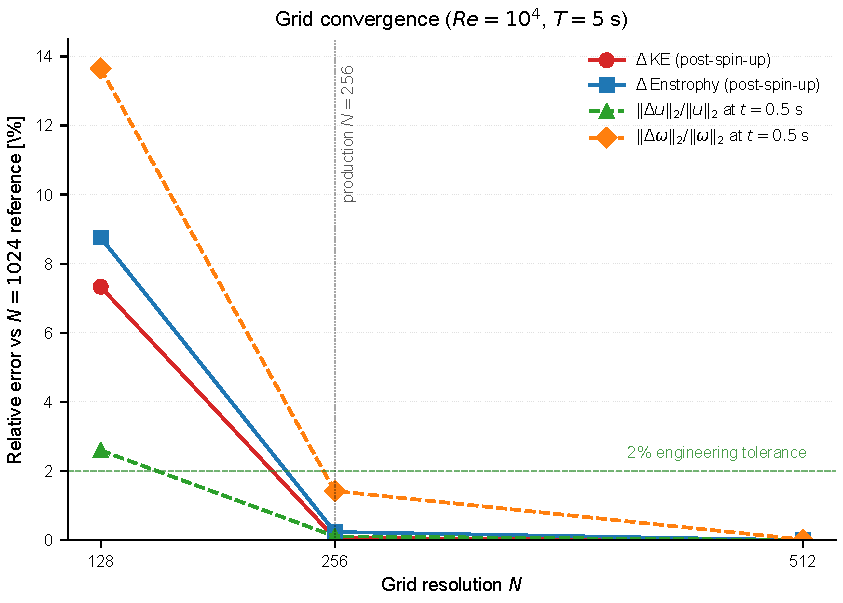
\includegraphics[width=0.72\textwidth]{figures/results/grid_indep_convergence.pdf}
    \caption{Relative error vs.\ grid resolution $N$ ($Re=10^4$, $T=5$~s) against the $N=1024$ reference. Lines: post-spin-up ($t \in [2,5]$~s) maximum relative differences of kinetic energy (KE, m$^2$/s$^2$) and enstrophy (1/s$^2$), and pointwise $L^2$ relative errors of $u$ and $\omega$ at $t=0.5$~s. Horizontal dashed line: $2\%$ tolerance; vertical dashed line: production resolution $N=256$. Values in Table~\ref{tab:dns_grid_indep}.}
    \label{fig:grid_indep_convergence}
\end{figure}

\begin{figure}[!htbp]
    \centering
    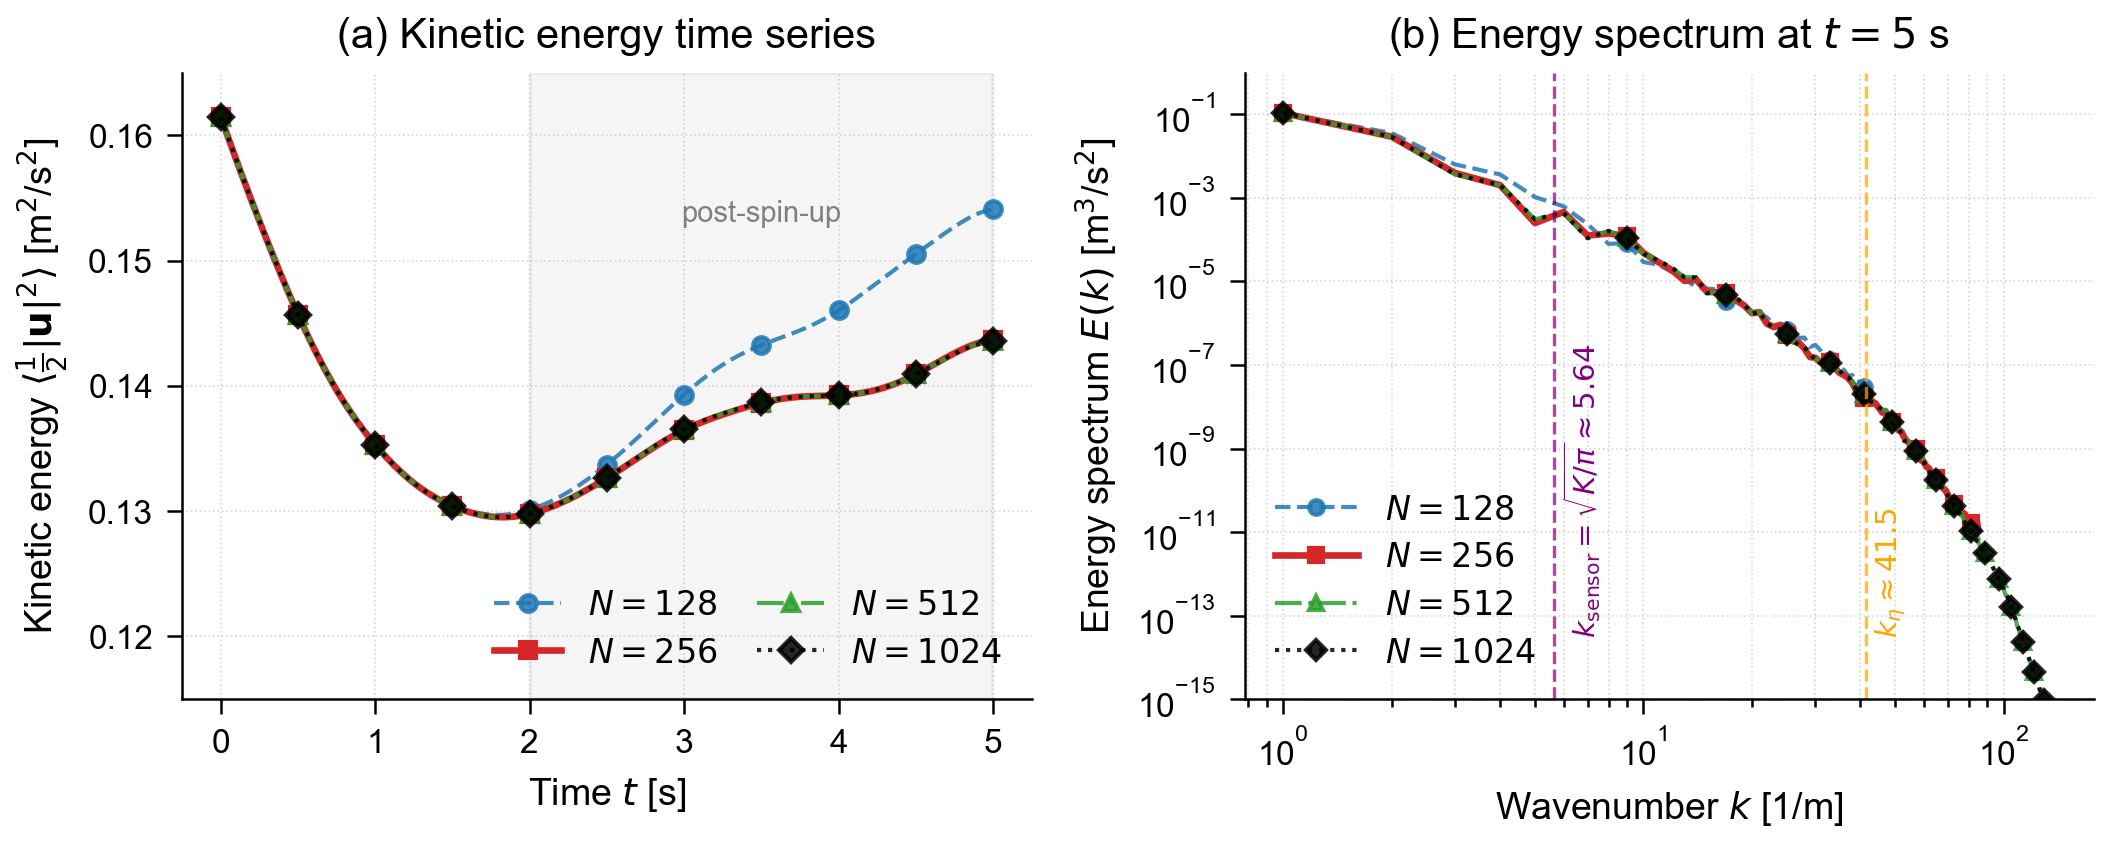
\includegraphics[width=\textwidth]{figures/results/grid_indep_main.png}
    \caption{Grid-independence supporting evidence. (a) Kinetic energy (m$^2$/s$^2$) vs.\ time $t$ (s) for $N \in \{128, 256, 512, 1024\}$; shaded band: post-spin-up window $t \in [2, 5]$~s. (b) Radial energy spectrum $E(k)$ (m$^3$/s$^2$) at $t=5$~s; vertical dashed lines: $K=100$ sensor Nyquist $k_{\rm sensor} = \sqrt{K/\pi} \approx 5.64$~m$^{-1}$ (purple) and dissipation wavenumber $k_\eta = 41.5$~m$^{-1}$ (orange).}
    \label{fig:grid_indep_main}
\end{figure}

\paragraph{Time-step, seed, and IC sensitivity.}
Three supplementary checks isolate non-spatial sources of error. Halving the time step at $N=256$, $T=0.5$ changes the solution by $7.0\times 10^{-6}$ ($160\times$ below the spatial error), confirming $\Delta t = 2.5\times 10^{-4}$ is temporally converged. A second seed reproduces the result: $N=256$-vs-$N=512$ post-spin-up KE agreement is $0.19\%$, within the $2\%$ engineering tolerance. Spectral truncation error is a property of discretisation rather than IC phase~\cite{Boyd2001}, and the $\approx 99\%$ sensor-band energy fraction holds for any forced-stationary trajectory at this $Re$, so the conclusions transfer to the production IC. Per-field log-log convergence and diagnostics across all four grids appear in Appendix~\ref{app:dns_grid_indep_supp}.

\section{LES for DNS-Free Sensor Placement}
\label{sec:les_placement}

In the LES-derived placement strategy (one of the placement options studied), a low-cost LES on a new scene supplies a POD basis from which QR-pivoting selects sensor positions; the physical flow then provides the sensor values. The DNS substitutes for the physical flow during controlled validation, but not for placement. The LES need not match the DNS pointwise: its sole role is to supply a POD snapshot matrix whose leading modes determine the QR-pivot indices. The LES and the DNS are therefore \emph{independent} realisations: they share the same $Re$, domain, and forcing but start from different random initial fields, so at high Reynolds number their trajectories decorrelate and never coincide pointwise at any matched time. Their integration horizons follow their roles, not each other. The LES is integrated long only so that its leading POD modes reach statistical convergence for placement (it is a statistical tool, not a trajectory to be matched); the DNS is the single target realisation to be reconstructed over the shorter window $t\in[0,5]$, from which the sensors read their values. Statistics therefore set the LES horizon and the reconstruction target sets the DNS horizon (the specific values appear in Tables~\ref{tab:dns_params} and~\ref{tab:les_params}).

\paragraph{Filtered equations and closure.}
The LES solves the spatially filtered incompressible Navier--Stokes equations,
\begin{subequations}
\label{eq:filtered_ns}
\begin{align}
    \nabla\!\cdot\!\bar{\mathbf{u}} &= 0, \label{eq:filtered_cont}\\
    \partial_t \bar{u}_i + \bar{u}_j\,\partial_j \bar{u}_i &= -\partial_i \bar{p} + \nu\,\nabla^2 \bar{u}_i - \partial_j \tau_{ij}^{\mathrm{SGS}} + f_i, \label{eq:filtered_mom}
\end{align}
\end{subequations}
on the same domain, viscosity, and forcing as the DNS. The high-wavenumber SGS drain is a spectral hyperviscosity term, used alone in the reference LES; the low-fidelity variant additionally applies a Bardina scale-similarity term~\cite{Bardina1980, Sagaut2006},
\begin{equation}
    \label{eq:bardina_hyperv}
    \begin{aligned}
    \mathcal{D}_{\rm hyper}(\bar{\mathbf{u}}) &= -\nu_h\,(-\nabla^2)^{p}\bar{\mathbf{u}}\quad(p=2), \\
    \tau_{ij}^{\mathrm{Bardina}} &= C_B (\widetilde{\bar{u}_i\,\bar{u}_j} - \widetilde{\bar{u}_i}\widetilde{\bar{u}_j})\quad(C_B = 1.0,\ \text{low-fidelity only}),
    \end{aligned}
\end{equation}
both chosen over Smagorinsky-type eddy-viscosity, which is poorly justified for 2D turbulence with a forced inverse cascade. The solver shares the DNS spatial discretisation (pseudo-spectral, $2/3$-rule dealiasing, fp64) but advances in time with an explicit second-order Runge--Kutta (RK2) scheme rather than the DNS's ETDRK4, with a conservatively small step ($\Delta t = 10^{-4}$~s, below the explicit hyperviscosity stability limit). It differs from the DNS in SGS closure, grid resolution, and time integrator. Reference and low-fidelity discretisation parameters are listed in Table~\ref{tab:les_params}.

\begin{table}[!htbp]
    \centering
    \caption{LES configuration at $Re=10\,000$. The sub-grid closure and the four discretisation parameters at the bottom differ between the reference and low-fidelity runs; values in brackets denote the low-fidelity setting. The governing equation and solver inherit the dimensional mapping of Table~\ref{tab:dns_params}.}
    \label{tab:les_params}
    \footnotesize
    \setlength{\tabcolsep}{5pt}
    \begin{tabularx}{\textwidth}{
        @{}>{\raggedright\arraybackslash}p{5.6cm}
        >{\raggedright\arraybackslash}X@{}
    }
    \toprule
    \textbf{Item} & \textbf{Setting (reference; [low-fidelity])} \\
    \midrule
    \multicolumn{2}{@{}l}{\emph{Governing equation}} \\
    Equation                   & Filtered NS,~\eqref{eq:filtered_ns}; $Re = 10\,000$, $\nu = 10^{-4}$~m$^2$/s \\
    Domain, forcing            & $[0,1]^2$~m$^2$, periodic; $\mathbf{f} = (A\sin 2\pi k_f y, 0)^T$ with $A=0.1$~m/s$^2$, $k_f=2$~m$^{-1}$ \\
    \midrule
    \multicolumn{2}{@{}l}{\emph{Sub-grid closure}} \\
    Form                       & hyperviscosity~\eqref{eq:bardina_hyperv}; $+$ Bardina scale-similarity~[low-fidelity] \\
    Coefficients               & hyperviscosity order $p = 2$; Bardina $C_B = 1.0$ (low-fidelity) \\
    Hyperviscosity tuning $\nu_h$ & per-run drain for a $> 10^6$ dissipation tail between $k_f$ and $k_{\max}^{\rm LES}$ \\
    \midrule
    \multicolumn{2}{@{}l}{\emph{Solver method}} \\
    Spatial / time / precision & spectral, $2/3$-rule dealiasing; explicit RK2 (Heun), $\Delta t = 10^{-4}$~s; fp64 \\
    Initial condition          & random Gaussian field + forced spin-up \\
    \midrule
    \multicolumn{2}{@{}l}{\emph{Discretisation (reference~/~[low-fidelity])}} \\
    Grid resolution $N_{\rm LES}$        & $256^2$~/~$[128^2]$ \\
    Effective $k_{\max}^{\rm LES}$       & $85.3$~m$^{-1}$~/~$[42.7$~m$^{-1}]$ \\
    Time horizon $T_{\rm end}$           & $50$~s ($26.5\,t_{\rm eddy}$)~/~$[15$~s, $7.5\,t_{\rm eddy}]$ \\
    Compute cost                         & $1\times$~/~$[1/16\times]$ \\
    \bottomrule
    \end{tabularx}
\end{table}

\paragraph{Verification.}
\label{subsec:les_verification}
Table~\ref{tab:les_verification} reports verification against three criterion groups. Spatial resolution targets resolved-band spectral overlap with DNS (within $2\times$ on $k\in[2, N_{\rm LES}/3]$) instead of the Pope-2000 criterion, since the SGS closure absorbs the unresolved stress; time-step stability uses a fixed $\Delta t = 10^{-4}$~s held below the explicit hyperviscosity limit (advective Courant $0.007$); statistical convergence is comfortable at $T_{\rm end}/t_{\rm eddy}=26.5$, with $\bar{\mathrm{KE}}(T)$ plateau within $5\%$ over the last $10$ snapshots, sub-window slope stationarity within $\pm 0.4$ slope units, and $\approx 17$ statistically independent POD samples (above the $\sim 10$-sample leading-mode threshold).

\begin{table}[!htbp]
    \centering
    \caption{LES verification for the reference LES ($N_{\rm LES}=256^2$, $T_{\rm end}=50$~s).}
    \label{tab:les_verification}
    \footnotesize
    \setlength{\tabcolsep}{5pt}
    \begin{tabularx}{\textwidth}{
        @{}>{\raggedright\arraybackslash}X
        >{\centering\arraybackslash}p{3.2cm}
        >{\centering\arraybackslash}p{1.8cm}
        >{\raggedright\arraybackslash}p{3.4cm}@{}
    }
    \toprule
    \textbf{Criterion} & \textbf{Threshold} & \textbf{Measured} & \textbf{Verdict} \\
    \midrule
    \multicolumn{4}{@{}l}{\emph{Spatial resolution}} \\
    Spectral overlap with DNS on $k\in[2, N_{\rm LES}/3]$ & within $2\times$       & within $2\times$ & $\checkmark$ leading modes aligned \\
    Pile-up at $k\to N_{\rm LES}/3$                       & none                   & none             & $\checkmark$ dealiasing intact \\
    \midrule
    \multicolumn{4}{@{}l}{\emph{Time-step adequacy and stability}} \\
    Advective Courant $U_{\rm rms}\Delta t/\Delta x$       & $\le 0.5$              & $0.007$          & $\checkmark$ \\
    Hyperviscous stability $\nu_h k_{\max}^{2p}\Delta t$   & $< 1$ (explicit RK2)   & $5\times 10^{-3}$ & $\checkmark$ \\
    Incompressibility $\Vert\nabla\!\cdot\!\bar{\mathbf{u}}\Vert_\infty$ & spectral round-off & $<10^{-10}$ & $\checkmark$ \\
    \midrule
    \multicolumn{4}{@{}l}{\emph{Statistical window}} \\
    Turnover coverage $T_{\rm end}/t_{\rm eddy}$          & $\ge 5$ for POD       & $26.5$           & $\checkmark$ $\gg 5$ \\
    Independent samples $T_{\rm end}/t_{\rm int}$         & $\ge 10$              & $\approx 17$     & $\checkmark$ POD-converged \\
    KE plateau over last $10$ snapshots                   & rel.\ change $<5\%$   & $<5\%$           & $\checkmark$ spin-up cleared \\
    \bottomrule
    \end{tabularx}
\end{table}

\paragraph{Predictability horizon.}
A same-initial-condition diagnostic bounds how long any reference-grade LES can match the DNS pointwise, substantiating the decorrelation premise stated above. The vorticity fields are co-located through $\approx 1\,t_{\rm eddy}$ and visibly separated by $\approx 2\,t_{\rm eddy}$ (Fig.~\ref{fig:les_vort_compare}). The reference LES, initialised from the DNS field at $t=0$ and integrated to $t=5$~s on the matched grid (shared $Re$, domain, and forcing), keeps its velocity relative-$L^2$ error against the DNS below $5\%$ for $0.59\,t_{\rm eddy}$ and below $20\%$ for $1.10\,t_{\rm eddy}$; beyond that, chaotic divergence and the closure difference dominate, and the full-field error peaks near $92\%$ (below the $\sqrt{2}$ fully-decorrelated level) by $t\approx 4$~s (Fig.~\ref{fig:les_predictability}). The energy-containing scales persist longest: the resolved-band ($k\le 5$) error follows the full-field error, and the velocity correlation stays above $0.9$ until $\approx 1.5\,t_{\rm eddy}$, while the small-scale vorticity correlation falls to $\approx 0.1$ by $t\approx 4$~s. The quadratic kinetic-energy and enstrophy ratios remain within $[0.74, 1.00]$ throughout. Even this most favourable, same-initial-condition pair loses pointwise agreement within about one-and-a-half eddy-turnover times, so the independent realisation used for placement (already decorrelated at $t=0$) never coincides pointwise; the placement information resides in the statistically converged POD structure, not in any matched-time field.

\begin{figure}[!htbp]
    \centering
    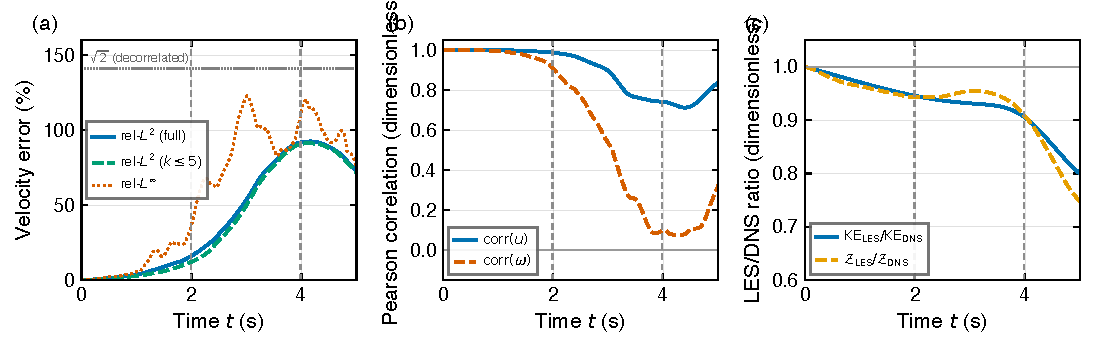
\includegraphics[width=\textwidth]{figures/results/les_sameic_predictability.pdf}
    \caption{Frame-by-frame comparison of a same-initial-condition reference LES against the DNS over $t\in[0,5]$~s ($Re=10^4$). (a) Velocity relative errors: full-field and resolved-band ($k\le 5$) relative-$L^2$, and relative-$L^\infty$ (\%); the grey dotted line marks the $\sqrt{2}$ fully-decorrelated level. (b) Pearson field correlations of velocity $u$ and vorticity $\omega$ (dimensionless). (c) LES/DNS ratios of kinetic energy and enstrophy $\mathcal{Z}=\langle\omega^2/2\rangle$ (dimensionless). Vertical dashed lines: one and two eddy-turnover times ($t_{\rm eddy}=1.99$~s).}
    \label{fig:les_predictability}
\end{figure}

\begin{figure}[!htbp]
    \centering
    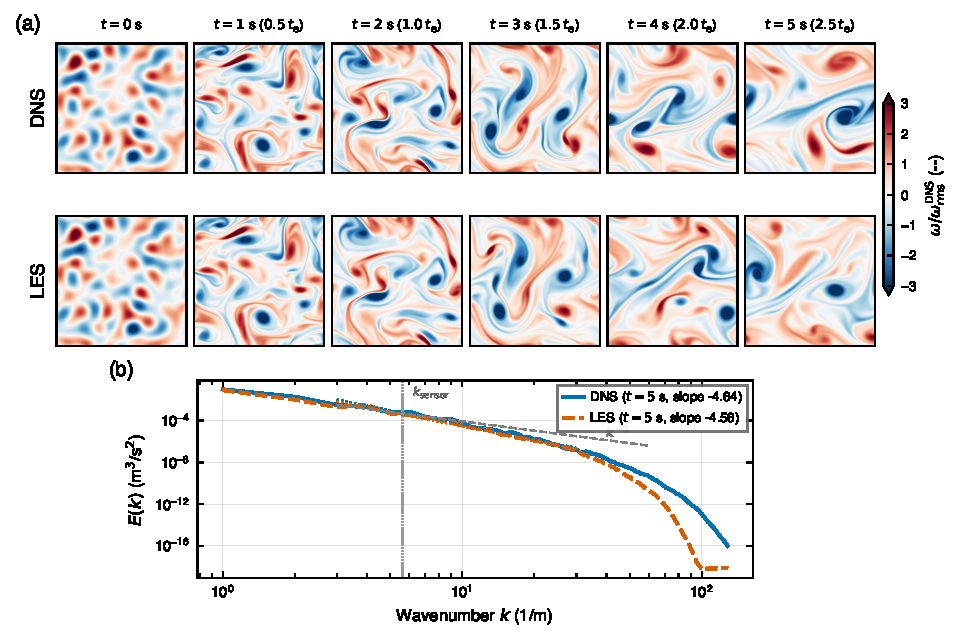
\includegraphics[width=\textwidth]{figures/results/dns_les_vorticity_compare.pdf}
    \caption{Same-initial-condition LES against the DNS ($Re=10^4$, periodic domain $[0,1]^2$~m). (a) Vorticity fields of the DNS (top) and the LES (bottom) at matched times $t\in\{0,1,2,3,4,5\}$~s; each time column is normalised by the DNS RMS vorticity, with colour showing $\omega/\omega_{\rm rms}^{\rm DNS}$ (dimensionless). (b) Radial energy spectrum $E(k)$ (m$^3$/s$^2$) of the LES and DNS at the matched final time $t=5$~s, with $k\in[3,30]$ slope fits and the $k^{-3}$ enstrophy-cascade reference; the vertical dotted line marks the $K=100$ sensor Nyquist $k_{\rm sensor}\approx 5.64$~m$^{-1}$. Eddy-turnover time $t_{\rm eddy}=1.99$~s.}
    \label{fig:les_vort_compare}
\end{figure}

\paragraph{Spectrum offset.}
Over the inertial range $k\in[3,30]$ the same-initial-condition LES and DNS energy spectra agree (slopes $-4.56$ and $-4.64$; Fig.~\ref{fig:les_vort_compare}b), while the LES energy falls below the DNS for $k\gtrsim 30$, where the hyperviscosity closure drains the small scales. This high-wavenumber offset bounds high-band reconstruction but not QR-pivot placement, which depends on the leading POD basis conditioning rather than the small-scale spectrum. The reference LES used for placement is integrated to $T_{\rm end}=50$ ($26.5\,t_{\rm eddy}$) for statistical convergence of the leading POD modes, since that convergence, not small-scale solver fidelity, governs the placement quality.

The LES-derived and DNS-oracle placements both target $K = 100$, with downstream KE MAPE within engineering tolerance (Table~\ref{tab:les_grid_independence}).

\begin{figure}[!htbp]
    \centering
    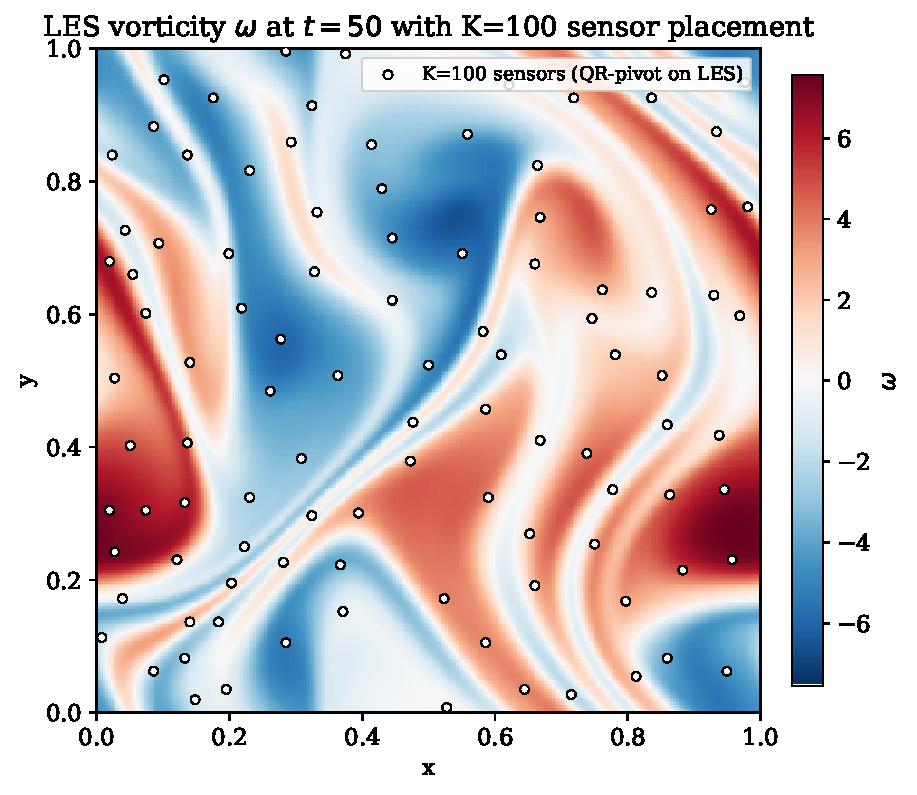
\includegraphics[width=0.7\linewidth]{figures/architecture/les_T50_vorticity_with_sensors.pdf}
    \caption{LES-derived sensor placement. Vorticity $\omega$ (1/s; $N_{\rm LES}=256$, $T_{\rm end}=50$) overlaid with $K=100$ QR-pivot sensor positions (markers) projected onto the DNS grid by nearest-neighbour mapping.}
    \label{fig:les_sensor_placement}
\end{figure}

\paragraph{Placement robustness to LES configuration.}
Grid independence in the DNS sense (Table~\ref{tab:dns_grid_indep}) does not transfer to the LES: the DNS converges to a resolved solution as $N$ increases, whereas an LES has no grid-converged limit short of DNS, since refining $N$ shifts the filter cutoff and the resolved/SGS split and thereby changes the resolved field itself. The relevant question is instead whether the \emph{placement} is robust to the LES configuration. The two LES runs compared (Table~\ref{tab:les_grid_independence}) differ not only in resolution ($N_{\rm LES}=256$ vs $128$) but also in closure (pure hyperviscosity vs Bardina-plus-hyperviscosity), hyperviscosity strength, and integration horizon ($T_{\rm end}=50$ vs $15$); despite this four-way change and a $16\times$ compute reduction, the downstream KE MAPE differs by only $0.04\%$ absolute ($\approx 0.3\%$ relative). The leading POD modes driving QR-pivot placement are therefore insensitive to the LES configuration, not merely to its resolution. The two retrainings here use a legacy single-seed, reduced-collocation configuration, so their absolute KE MAPE ($\approx 12\%$) sits above the final-protocol baseline; only the near-zero difference between them, the placement-robustness quantity, is used as evidence.

\begin{table}[!htbp]
    \centering
    \caption{LES configuration robustness: downstream KE MAPE after the full pipeline (LES POD basis $\to$ QR-pivot $\to$ sensor measurement $\to$ PI-CON retraining) under two LES runs that differ in resolution, closure, hyperviscosity strength, and integration horizon. The $E(k)$ slope is measured for $k>k_f$ (1/s units); the low-fidelity $-14$ reflects over-dissipation, and the $\approx 0.3\%$ relative difference lies at the evaluator noise floor. Both rows use a legacy single-seed, reduced-collocation retraining, so the absolute KE MAPE exceeds the final-protocol baseline; the placement-robustness claim rests on their relative difference, not the absolute level.}
    \label{tab:les_grid_independence}
    \footnotesize
    \setlength{\tabcolsep}{5pt}
    \begin{tabular}{lccccc}
    \toprule
    \textbf{Configuration} & \textbf{$N_{\rm LES}$} & \textbf{$T_{\rm end}$ (s)} & \textbf{Closure} & \textbf{$E(k)$ slope} & \textbf{KE MAPE} \\
    \midrule
    Reference LES    & $256^2$ & $50$ & hyperviscosity      & $-6.46$ & $12.36\%$ \\
    Low-fidelity LES & $128^2$ & $15$ & Bardina $+$ hyperv. & $-14$   & $12.40\%$ \\
    \midrule
    Difference       & --     & --  & --                 & --     & \textbf{$\approx 0.3\%$ rel.} \\
    \bottomrule
    \end{tabular}
\end{table}

\section{Sensor Data Construction}
\label{sec:sensor_data}

\paragraph{Pipeline alignment.}
For the LES-derived placement, data construction follows the deployment order: the LES determines where sensors are placed (positions only; the LES supplies no sensor values), and the physical flow determines what they measure. In this controlled study a DNS field stands in for the real-world flow, sampled at the $K$ sensor positions alone, so the model receives time-stamped $u,v$ values at fixed locations; the full DNS field is never read during training.

\paragraph{Sensor placement.}
The QRCP-on-POD-basis procedure of \S\ref{sec:sensor_placement} selects $K = 100$ grid indices and their physical coordinates from $\mathbf{X}\in\mathbb{R}^{N\times 201}$.

\paragraph{Sensor measurement values.}
Each sensor record contains time stamps and the corresponding $u,v$ velocities at the selected positions, with $N_t = 201$ aligned to the DNS frames. Vorticity is a derived diagnostic and pressure a model-internal variable; neither is used as supervision.

\paragraph{Normalization.}
Sensor values are standardized per channel,
\begin{equation}
    \hat{u}_{k,n} \;=\; \frac{u_{k,n} - \mu_u}{\sigma_u},\quad \hat{v}_{k,n} \;=\; \frac{v_{k,n} - \mu_v}{\sigma_v},
\end{equation}
where $\mu, \sigma$ are computed from all $K\cdot N_t$ measurements. The query-side prediction is inverse-transformed to recover the physical scale. The Reynolds number is normalized as $Re_{\text{norm}} = (Re - 5\,500) / 4\,000$, with offset and scale matching the approximate median and standard deviation of $\{100, 1\,000, 10\,000, 100\,000\}$ for multi-$Re$ training.

\paragraph{Train/validation split.}
At each step, an $80\%$ random subset of (time-index, space-index, channel-index) triples forms the training mini-batch; the remaining $20\%$ is held out as an in-sample interpolation check. The primary evaluation is the a posteriori field-reconstruction error against DNS (\S\ref{sec:eval_metrics}). Because the sensor (branch) input is identical for both subsets, this split monitors only transductive overfitting, memorising the specific space--time query coordinates seen in training; it is a sensor-consistency diagnostic and does not test generalisation to unseen sensor streams or flow conditions.

\section{Evaluation Metrics}
\label{sec:eval_metrics}

All metrics are computed post-training on a $128\times 128$ grid (the stored $256\times 256$ DNS snapshots are downsampled to $128^2$) so that finite-difference derivatives (divergence, vorticity) are evaluated below the stored-grid Nyquist wavenumber, where the central-difference stencil is uncontaminated by spectral-truncation noise near $k\to k_{\max}^{256}$.

\subsection{Field-Level Errors}

The error budget is reported at three levels: (i) a global, time-averaged $L_2$ norm; (ii) a pointwise worst-case ($L_\infty$) norm capturing localised peak error; (iii) a snapshot error at the final time $t^\star = T = 5$, the most demanding instant under the chaotic horizon (the trajectory spans $\approx 2.5$ eddy-turnover times). The definitions follow the PINN sparse-sensor reconstruction literature~\cite{Raissi2019JCP,Wang2024JMLR} and classical CFD validation practice~\cite{Pope2000}.

\paragraph{Relative $L_2$ error.}
For $\phi \in \{u, v, \omega, p\}$, following the normalised $L_2$ convention of~\cite{Raissi2019JCP},
\begin{equation}
    \mathrm{rel}\,L_2(\phi) \;=\; \frac{\Vert \phi_{\text{pred}} - \phi_{\text{DNS}}\Vert_2}{\Vert \phi_{\text{DNS}}\Vert_2},
\end{equation}
reported as a time-averaged value (mean over $t\in[0,T]$).

\paragraph{Relative $L_\infty$ (maximum) error.}
The worst-case pointwise discrepancy normalised by the maximum DNS amplitude,
\begin{equation}
    \label{eq:rel_linf}
    \mathrm{rel}\,L_\infty(\phi) \;=\; \frac{\max_{\mathbf{x},\,t}\,|\phi_{\text{pred}}(\mathbf{x},t) - \phi_{\text{DNS}}(\mathbf{x},t)|}{\max_{\mathbf{x},\,t}\,|\phi_{\text{DNS}}(\mathbf{x},t)|},
\end{equation}
captures localised peak discrepancies (e.g.\ unresolved shear-layer cusps) that the global $L_2$ averages out. The maximum runs over the $128^2$ grid and all $201$ time stamps.

\paragraph{Snapshot error at $t^\star = T$.}
The relative $L_2$ error of the final snapshot is reported separately, since forward integration accumulates phase error along the chaotic trajectory and $t^\star = 5$ is the most demanding instant:
\begin{equation}
    \label{eq:rel_l2_tstar}
    \mathrm{rel}\,L_2^{\,t^\star}(\phi) \;=\; \frac{\Vert \phi_{\text{pred}}(\cdot,\,t^\star) - \phi_{\text{DNS}}(\cdot,\,t^\star)\Vert_2}{\Vert \phi_{\text{DNS}}(\cdot,\,t^\star)\Vert_2}.
\end{equation}
A bounded snapshot error at $t^\star$ indicates the operator retains physical fidelity at the trajectory end, not only in time-averaged statistics.

\paragraph{Kinetic-energy MAPE.}
The integrated kinetic energy is the canonical CFD validation observable for turbulent statistics~\cite{Pope2000}. Its Mean Absolute Percentage Error (MAPE) is
\begin{equation}
    \mathrm{KE}(t) \;=\; \tfrac{1}{2}\int_\Omega \big(u^2 + v^2\big)\,d\mathbf{x},\qquad
    \mathrm{KE\_MAPE}(t) = \frac{|\mathrm{KE}_{\text{pred}}(t) - \mathrm{KE}_{\text{DNS}}(t)|}{\mathrm{KE}_{\text{DNS}}(t)}.
\end{equation}
The scalar reported in tables and figures is the time-mean $\overline{\mathrm{KE\_MAPE}} = \tfrac{1}{|T|}\sum_t \mathrm{KE\_MAPE}(t)$ over the evaluation window $t\in[0,5]$~s. This time-averaged relative error of $\mathrm{KE}(t)$ is the quantity referred to as the \emph{KE relative error} elsewhere in the text; the two names denote the same metric.

\paragraph{Enstrophy relative error.}
A second-order vorticity quantity with $\omega = \partial_x v - \partial_y u$:
\begin{equation}
    \mathrm{Ens}(t) \;=\; \tfrac{1}{2}\int_\Omega \omega^2\,d\mathbf{x},\qquad
    \mathrm{Ens\_rel\_err}(t) \;=\; \frac{|\mathrm{Ens}_{\text{pred}}(t) - \mathrm{Ens}_{\text{DNS}}(t)|}{\mathrm{Ens}_{\text{DNS}}(t)}.
\end{equation}

\subsection{Physics Consistency}

\paragraph{Divergence $L_2$.}
The incompressibility residual, evaluated on a finite-difference grid where the spectral-exact constraint $\nabla\!\cdot\!\mathbf{u} = 0$ is no longer at machine precision, is reported as both an absolute norm and a scale-normalised ratio. The ratio follows the dimensional-analysis convention of normalising solenoidal violations by the local strain-rate norm, enabling cross-resolution comparison~\cite{Pope2000,Moin1998AIAA}:
\begin{equation}
    \mathrm{div}\_L_2(t) \;=\; \big\Vert \partial_x u_{\text{pred}} + \partial_y v_{\text{pred}} \big\Vert_2.
\end{equation}
The spectral DNS is divergence-free in spectral space but not in finite-difference space, giving an evaluation-grid floor $\Vert\nabla\cdot\mathbf{u}\Vert_2 \approx 0.092$ ($1.04\%$ of the DNS strain rate $\Vert\nabla\mathbf{u}\Vert_F^{\rm DNS}$; Table~\ref{tab:dns_verification}). This floor is the truncation error of the second-order central-difference operator on the $128^2$ evaluation grid and scales with the resolved high-wavenumber content: spectrally low-pass filtering the DNS reference to $k\le 16$ lowers it to $0.38\%$, and to $k\le 5$ to $0.07\%$. The floor is therefore a property of the field's bandwidth under the chosen operator, not an absolute incompressibility limit; a reconstruction confined to low wavenumbers is expected to register a smaller value for this reason alone. The relative divergence ratio
\begin{equation}
    \mathrm{div}\_\mathrm{ratio} \;=\; \Vert\nabla\cdot\mathbf{u}_{\rm pred}\Vert_2 \big/ \Vert\nabla\mathbf{u}\Vert_F^{\rm DNS}
\end{equation}
places model values on the same scale, with $\Vert\nabla\mathbf{u}\Vert_F^{\rm DNS} = 8.898$ on the evaluation grid (\S\ref{subsec:dns_verification}).

\paragraph{NS residual r.m.s.}
The root-mean-square of the NS momentum and continuity residuals at $N_c$ collocation points,
\begin{equation}
    \label{eq:ns_rms}
    \mathrm{NS\_rms}_\phi \;=\; \sqrt{\frac{1}{N_c}\sum_{j=1}^{N_c} \mathcal{R}_\phi^2(\mathbf{x}_j,t_j)}, \quad \phi \in \{u,\, v,\, c\},
\end{equation}
with $\mathcal{R}_u$, $\mathcal{R}_v$, $\mathcal{R}_c$ defined in \eqref{eq:res_u}--\eqref{eq:cont_res}. The continuity variant is also written $\mathrm{div\_rms}$. Values are compared against the DNS reference computed on the downsampled grid.

\subsection{Spectral Diagnostics}

\paragraph{Per-band relative error.}
The KE spectrum is grouped along the K=100 sensor Nyquist cutoff $k_{\max}^{\rm sensor} = \lfloor \sqrt{K/\pi} \rfloor = \lfloor 5.64 \rfloor = 5$ (the integer band edge; the unfloored $\sqrt{K/\pi}\approx 5.64$ appears in the spectral plots). This cutoff is the two-dimensional Nyquist wavenumber for $K$ samples over a unit-area domain (one sample per $\pi/K$ wavenumber cell), the spatial-sampling analogue of the one-dimensional Nyquist limit; above it the $K$ sensors cannot constrain independent Fourier modes. The bands are: a low band ($k \le 5$, below the sensor Nyquist cutoff $k_{\max}^{\rm sensor}\approx 5.64$, which carries $\approx 99\%$ of the total energy at $t=5$, and $\approx 95\%$ time-averaged over $t\in[0,5]$, the lower mean reflecting the broadband initial condition during spin-up; fully sensor-resolvable), a mid band ($5 < k \le 16$, transitional), and a high band ($k > 16$, above the sensor Nyquist cutoff). For each band,
\begin{equation}
    \mathrm{band\_rel\_err}(t) \;=\; \frac{|E_{\text{band, pred}}(t) - E_{\text{band, DNS}}(t)|}{E_{\text{band, DNS}}(t)}.
\end{equation}

\paragraph{Forcing-mode amplitude and phase.}
Since $k_f = 2$ carries the sustained energy injection, its reconstruction is reported separately. From the Fourier coefficient $\hat{u}_{k_f}$,
\begin{equation}
    \mathrm{amp\_ratio}(t) \;=\; \frac{|\hat{u}^{\text{pred}}_{k_f}|}{|\hat{u}^{\text{DNS}}_{k_f}|},\quad
    \mathrm{phase\_err}(t) \;=\; \arg(\hat{u}^{\text{pred}}_{k_f}) - \arg(\hat{u}^{\text{DNS}}_{k_f}).
\end{equation}
The ideal values are $\mathrm{amp\_ratio} = 1$ and $\mathrm{phase\_err} = 0$.

\paragraph{Time-segment decomposition.}
Metrics are also reported as means over three segments: early ($t<1$), mid ($1\le t<3$), late ($t\ge 3$).

\paragraph{Wavelet-based multi-scale error diagnostic.}
Complementing the Fourier-band diagnostics, a 2D Daubechies-4 wavelet decomposition is applied to the reconstructed field. The wavelet metric decomposes the relative $L_2$ error by level, providing the spatial localisation that the global Fourier spectrum lacks. Full details are in Appendix~\ref{app:wavelet_diag}.

\subsection{Train/Validation Split Metrics}
To detect transductive overfitting, KE MAPE is reported over the training window $t\in[0, 4]$ and the validation window $t\in[4, 5]$ separately.

\section{Ablation and Reference Comparisons}
\label{sec:baselines}

The final result set contextualises PI-CON through matched architecture ablations and reference-only diagnostics. The classical-interpolation baselines (RBF, IDW, and divergence-free trigonometric least squares) are regenerated on the final LES-derived placement and reported in Appendix~\ref{app:fair_baselines}; older Standard-PINN development comparisons are not used as thesis evidence because they were not regenerated under the final $20\,000$-iteration, $1024$-collocation PI-CON protocol.

\paragraph{Matched architecture ablations.}
The four neural variants reconstruct the field from the same $K=100$ sensor stream as PI-CON and require no DNS full-field access at training or inference:
\begin{itemize}
    \item \textbf{Vanilla DeepONet} (B0): the same operator backbone without CfC temporal encoding and without cross-attention; the architectural reference for the $2\times2$ ablation matrix.
    \item \textbf{CfC-only} (B1): B0 plus CfC temporal encoding, but without cross-attention.
    \item \textbf{Cross-attention-only} (B2): B0 plus query-conditional cross-attention, but without CfC temporal encoding.
    \item \textbf{Full PI-CON} (B3): CfC temporal encoding and query-conditional cross-attention together.
\end{itemize}

\paragraph{Reference-only baseline (not engineering-transferable).}
\textbf{Gappy POD} requires the full DNS snapshot matrix to build its POD basis and is \emph{not engineering-transferable} under the deployment regime of \S\ref{sec:engineering_constraint}; it is reported only as an upper reference for spectral-truncation reconstruction quality, not as a comparable method. The \textbf{forward-CFD initial-condition reconstruction} likewise needs offline DNS snapshots for its POD basis and is labelled accordingly.

\section{Open-Source Availability}
\label{sec:impl_env}

The implementation is available at \url{https://github.com/latteine1217/pi-lnn}. Statistical comparisons use five independent seeds with Welch's two-sample $t$-test and Cohen's $d$ effect size.

\chapter{Results and Discussion}
\label{ch:results}

This chapter reports the main reconstruction result, the validation studies, and how sensing configuration governs reconstruction quality. The pipeline is: sensor placement $\to$ sensor measurements (here, DNS samples) $\to$ sensor-only physics training $\to$ continuous field reconstruction. Placement uses a low-cost LES in the main pipeline and is compared with two alternatives. The chapter proceeds from the headline result, field and spectral characterisation, and architectural ablation; through sensor count, placement, and noise studies; to a higher-Reynolds feasibility case, diagnostic boundaries, and inference cost.

\section{Main Result on $Re=10\,000$ Kolmogorov Flow}
\label{sec:main_result}

The main result uses the DNS-free LES-derived placement (one of the three placement strategies studied; \S\ref{sec:placement_analysis}): a one-head PI-CON readout, $1024$ physics-collocation points, and $K=100$ sensor locations selected from a long-horizon ($T_{\rm end}=50$~s) LES trajectory rather than DNS. Both the LES-pivot and DNS-pivot configurations are evaluated over the same $n=5$ random seeds at $20\,000$ training iterations, differing only in the sensor-placement source; Table~\ref{tab:main_metrics} therefore isolates placement quality.

\begin{table}[!htbp]
    \centering
    \caption{Main result and DNS-oracle placement reference at $Re=10\,000$, $K=100$, $n=5$ seeds, $20\,000$ iterations. Columns differ only in sensor-placement source. Values: mean $\pm$ sample standard deviation over seeds $\{42, 1, 2, 3, 4\}$. The KE, $u$, $v$, and $\omega$ errors are time-averaged over $t\in[0,T]$ (KE is MAPE). Relative-error metrics are percentages; divergence ratio $= \Vert\nabla\!\cdot\!\mathbf{u}\Vert_2 / \Vert\nabla\mathbf{u}\Vert_F^{\rm DNS}$.}
    \label{tab:main_metrics}
    \footnotesize
    \setlength{\tabcolsep}{3pt}
    \begin{tabularx}{\textwidth}{
        >{\raggedright\arraybackslash}p{3.2cm}
        >{\centering\arraybackslash}X
        >{\centering\arraybackslash}X
    }
    \toprule
    \textbf{Metric} & \textbf{LES placement} & \textbf{DNS-oracle placement} \\
    & \textbf{LES sensors ($n=5$, 20k iter)} & \textbf{DNS sensors ($n=5$, 20k iter)} \\
    \midrule
    Sensor placement source & LES $T=50$ & DNS oracle \\
    Physics collocation points & $1024$ & $1024$ \\
    KE MAPE & $5.71 \pm 0.11\%$ & $\mathbf{4.68 \pm 0.06\%}$ \\
    $u$ rel-$L_2$ & $\mathbf{13.65 \pm 0.06\%}$ & $15.34 \pm 0.06\%$ \\
    $v$ rel-$L_2$ & $\mathbf{17.52 \pm 0.10\%}$ & $18.10 \pm 0.03\%$ \\
    $\omega$ rel-$L_2$ & $\mathbf{41.79 \pm 0.12\%}$ & $42.41 \pm 0.12\%$ \\
    Divergence ratio & $0.39 \pm 0.006\%$ & $0.36 \pm 0.004\%$ \\
    $k_f$ amplitude ratio & $0.991 \pm 0.005$ & $0.986 \pm 0.005$ \\
    \bottomrule
    \end{tabularx}
\end{table}

\paragraph{Comparison boundary.}
The closest published sensor-only-with-physics comparison, Mo and Magri~\cite{Mo2025PRF}, addresses the same regime with a fixed-grid convolutional backbone; supervision-regime and architectural caveats are discussed in \S\ref{sec:literature}. Classical interpolation and older development baselines are not used as Chapter~\ref{ch:results} evidence because their reported numbers were not regenerated under the final $20\,000$-iteration, $1024$-collocation PI-CON protocol.

\paragraph{Time-segment decomposition.}
Table~\ref{tab:time_local} reports early, mid, and late segment averages from the main pipeline, diagnosing when reconstruction is hardest without altering the baseline definition; the worst single-time KE MAPE is $29.96\%$, at $t = 0.10$~s.

\paragraph{Discussion.}
The main row in Table~\ref{tab:main_metrics} uses no DNS full field for sensor placement or training supervision; sensor values are the DNS stand-in sampled only at the $K$ positions. Against the DNS-oracle reference, placement shows an integral/pointwise trade-off: the oracle has lower KE error ($4.68\%$ vs $5.71\%$), while LES-derived placement has lower pointwise velocity error ($u$ rel-$L_2$ $13.65\%$ vs $15.34\%$, $v$ rel-$L_2$ $17.52\%$ vs $18.10\%$). All strategies remain within the $10\%$ target: random placement gives KE $7.95\%$, LES-derived placement $5.71\%$, and the non-deployable DNS oracle $4.68\%$. LES-derived placement is therefore adopted as the reference DNS-free configuration because it improves over random by $2.24$ KE percentage points and reduces placement-induced variance roughly sixfold (\S\ref{sec:placement_analysis}).

The divergence ratio of $0.39\%$ confirms the continuity constraint is active, matching the finite-difference floor of a DNS field band-limited to the reconstruction's resolved bandwidth (\S\ref{sec:sub_dns_div}; Fig.~\ref{fig:main_trajectories}, second panel). The energy-dominant low-wavenumber band (sensor-count Nyquist scale $k_{\max}^{\rm sensor}\approx 5.64$, carrying $\approx 99\%$ of kinetic energy at $t=5$; \S\ref{subsec:nyquist_scaling}) recovers to single-digit relative error (Fig.~\ref{fig:band_err}), within the $10\%$ engineering target of O1.

Error is largest over the first half-second, consistent with the difficulty of reconstructing the initial condition from sensor history alone, and declines steadily thereafter (Fig.~\ref{fig:main_trajectories}, first panel). The time-mean KE error in Table~\ref{tab:main_metrics} therefore aggregates a decaying transient rather than a stationary error level. The sensor-count sweep in \S\ref{subsec:nyquist_scaling} is single-seed, but uses the final PI-CON protocol and is interpreted only as a bandwidth trend.

\begin{figure}[!htbp]
    \centering
    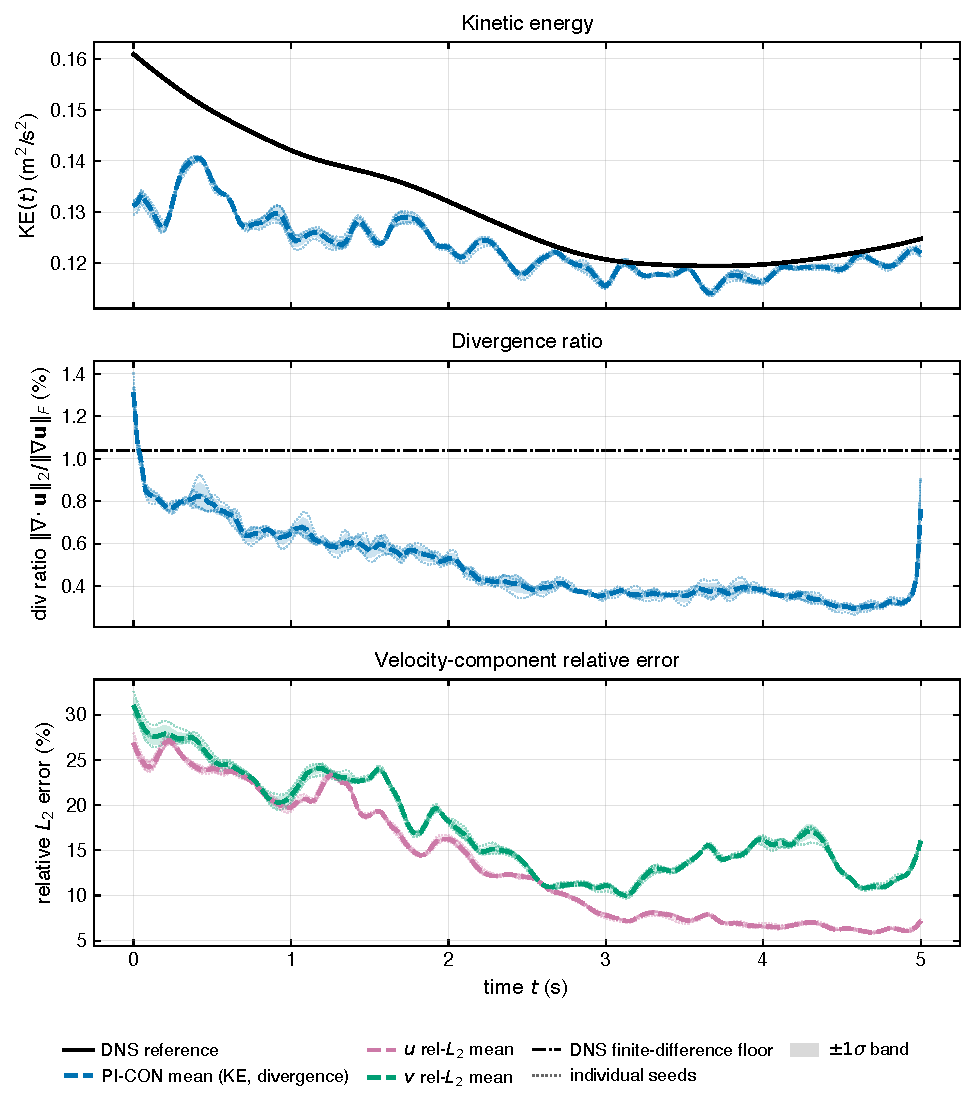
\includegraphics[width=\linewidth]{figures/results/main_trajectories.pdf}
    \caption{LES-pivot main-pipeline trajectory diagnostics over $n=5$ seeds (42, 1, 2, 3, 4), versus time $t$ (s). First panel: kinetic energy $\mathrm{KE}(t)$ (m$^2$/s$^2$). Second panel: divergence ratio $\Vert\nabla\!\cdot\!\mathbf{u}_{\rm pred}\Vert_2 / \Vert\nabla\mathbf{u}\Vert_F^{\rm DNS}$ (\%), with the DNS finite-difference floor. Third panel: $u$ and $v$ root-mean-square error (m/s). Fourth panel: DNS component magnitudes $\Vert u_{\rm DNS}\Vert_{\rm rms}$ and $\Vert v_{\rm DNS}\Vert_{\rm rms}$ (m/s), which are the denominators of the component relative $L_2$ errors reported in Table~\ref{tab:main_metrics}. In the first three panels the dashed line is the across-seed mean, dotted lines are individual seeds, and the shaded band is $\pm 1\sigma$; the DNS reference is solid.}
    \label{fig:main_trajectories}
\end{figure}

\begin{table}[!htbp]
    \centering
    \caption{Time-segment decomposition of the LES-pivot main result. Early: $t<1$~s; Mid: $1\le t<3$~s; Late: $t\ge 3$~s.}
    \label{tab:time_local}
    \small
    \begin{tabular}{lccc}
    \toprule
    \textbf{Metric} & \textbf{Early ($t<1$)} & \textbf{Mid ($1\le t<3$)} & \textbf{Late ($t\ge 3$)} \\
    \midrule
    $u$ rmse & 0.112 & 0.053 & 0.042 \\
    $v$ rmse & 0.102 & 0.051 & 0.033 \\
    $\omega$ rmse & 6.63 & 3.55 & 2.34 \\
    KE MAPE & $\sim 14\%$ & $\sim 5\%$ & $\sim 5\%$ \\
    \bottomrule
    \end{tabular}
\end{table}

\paragraph{Multi-seed statistical confirmation.}
\label{sec:statistical_significance}
The main result is checked against seed variability with an $n=5$ ensemble, which also provides a training-variability estimate.

\paragraph{Multi-seed training variability.}
The multi-seed training protocol follows a \emph{deep ensemble}~\cite{Lakshminarayanan2017DeepEnsembles}: training $n=5$ models from different random initialisations yields both a point estimate (the across-seed mean) and an empirical measure of training-induced variability (the across-seed standard deviation), capturing sensitivity to random initialisation and to the stochastic physics-collocation sampling schedule~\cite{Psaros2023UQ}. Here $n=5$ seeds yield a KE standard deviation of $0.11$ percentage points ($1.9\%$ relative scatter). This quantifies seed-and-collocation variability rather than a calibrated predictive uncertainty: no coverage or calibration of the spread is claimed.

To confirm the main result is not a seed artefact, the B3 LES-pivot configuration is trained over five seeds ($42, 1, 2, 3, 4$) at the main-pipeline $20\,000$-iteration budget. Table~\ref{tab:multiseed} reports per-seed values.

\begin{table}[!htbp]
    \centering
    \caption{Per-seed metrics for the B3 LES-pivot pipeline at $Re=10\,000$, $K=100$, $1024$ collocation points, $20\,000$ iterations. Last row: across-seed mean $\pm$ standard deviation. The KE, $u$, $v$, and $\omega$ errors are time-averaged over $t\in[0,T]$ (KE is MAPE); the $k_f$ amplitude ratio is reported at the final time $t=5$.}
    \label{tab:multiseed}
    \footnotesize
    \setlength{\tabcolsep}{3pt}
    \begin{tabularx}{\textwidth}{
        >{\raggedright\arraybackslash}p{1.6cm}
        >{\centering\arraybackslash}X
        >{\centering\arraybackslash}X
        >{\centering\arraybackslash}X
        >{\centering\arraybackslash}X
        >{\centering\arraybackslash}X
        >{\centering\arraybackslash}X
    }
    \toprule
    \textbf{Seed} & \textbf{KE \%} & \textbf{$u$ $L_2$ \%} & \textbf{$v$ $L_2$ \%} & \textbf{$\omega$ $L_2$ \%} & \textbf{div ratio \%} & \textbf{$k_f$ amp} \\
    \midrule
    $42$ ($_a$) & $5.9035$ & $13.59$ & $17.53$ & $41.66$ & $0.39$ & $0.9973$ \\
    $1$  ($_b$) & $5.6751$ & $13.74$ & $17.70$ & $41.95$ & $0.40$ & $0.9852$ \\
    $2$  ($_c$) & $5.6491$ & $13.63$ & $17.48$ & $41.67$ & $0.40$ & $0.9871$ \\
    $3$  ($_d$) & $5.7144$ & $13.66$ & $17.46$ & $41.83$ & $0.39$ & $0.9915$ \\
    $4$  ($_e$) & $5.5882$ & $13.65$ & $17.44$ & $41.75$ & $0.39$ & $0.9957$ \\
    \midrule
    \textbf{mean$\pm$std} & $\mathbf{5.71 {\pm} 0.11}$ & $\mathbf{13.65 {\pm} 0.06}$ & $\mathbf{17.52 {\pm} 0.10}$ & $\mathbf{41.79 {\pm} 0.12}$ & $\mathbf{0.39 {\pm} 0.006}$ & $\mathbf{0.991 {\pm} 0.005}$ \\
    \bottomrule
    \end{tabularx}
\end{table}

\paragraph{Reproducibility.}
The seed-to-seed KE standard deviation is $0.11$ percentage points ($1.9\%$ relative to the mean); all five seeds fall within a $0.32$ percentage-point window ($5.59$--$5.90\%$). Pointwise $u$-$L_2$ and $v$-$L_2$ are tighter still ($\sigma=0.06\%$ and $0.10\%$, both below $1\%$ relative scatter). The divergence ratio is reproducible to two decimal places ($0.39 \pm 0.006\%$), confirming it is a property of the architecture--AL recipe rather than any individual seed (\S\ref{sec:sub_dns_div}).

\paragraph{Architectural significance.}
The architectural advantage holds at budget parity. With all four ablation cells trained at the matched $1\,024$-collocation $20\,000$-iteration $n=5$-seed regime, a Welch $t$-test between B0 (Vanilla DeepONet, $8.23 \pm 0.22\%$) and B3 (Full PI-CON, $5.71 \pm 0.11\%$) gives a KE gap of $-2.52$ percentage points ($t=22.9$, $p=3.0\times10^{-7}$, Cohen's $d=14.5$): the gain is significant and not an artefact of seed count or iteration budget. The full $2\times2$ component decomposition appears with the ablation matrix (\S\ref{sec:baseline_comparison}).

\section{Field, Vorticity, and Low-Order Statistics}
\label{sec:visual}

\begin{figure}[!htbp]
    \centering
    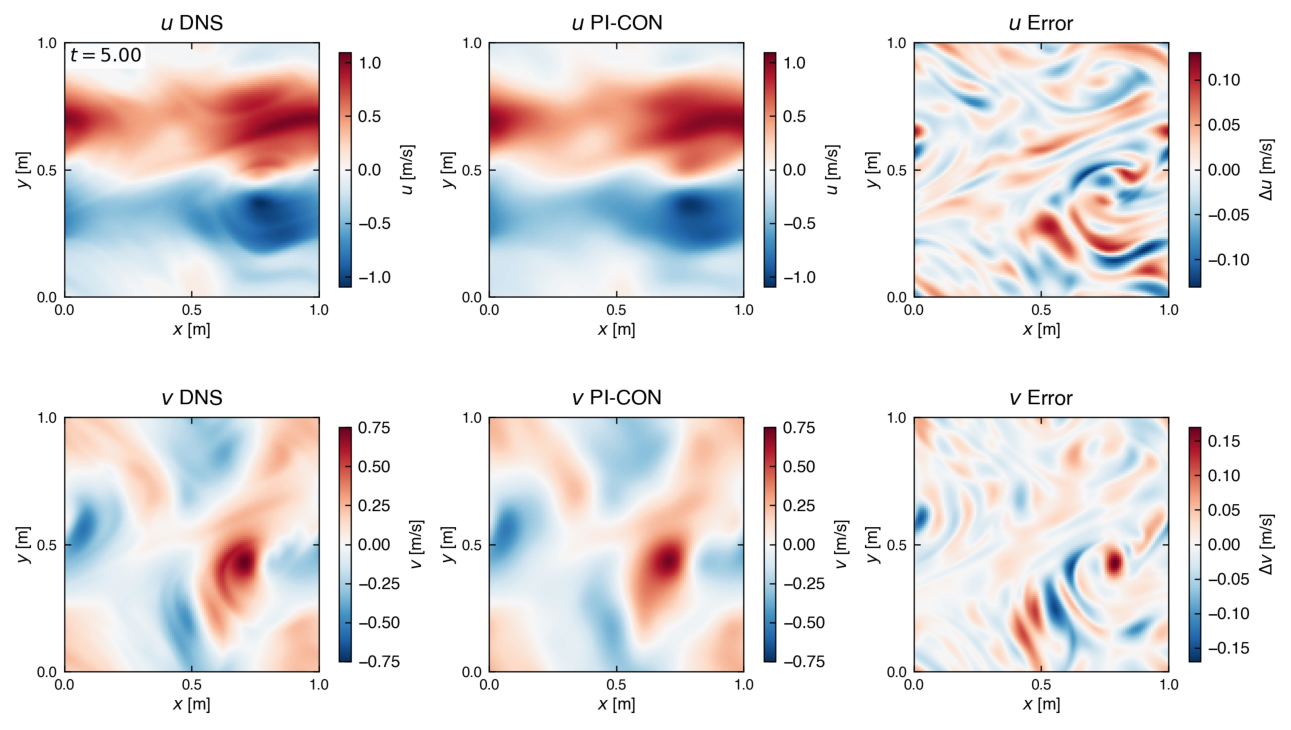
\includegraphics[width=0.95\linewidth]{figures/results/field_comparison_t5.pdf}
    \caption{Velocity and vorticity fields at $t=5$ (seed 42). Columns: DNS reference, PI-CON prediction, absolute error. Rows: $u$ (m/s), $v$ (m/s), vorticity $\omega$ (1/s).}
    \label{fig:field_t5}
\end{figure}

\begin{figure}[!htbp]
    \centering
    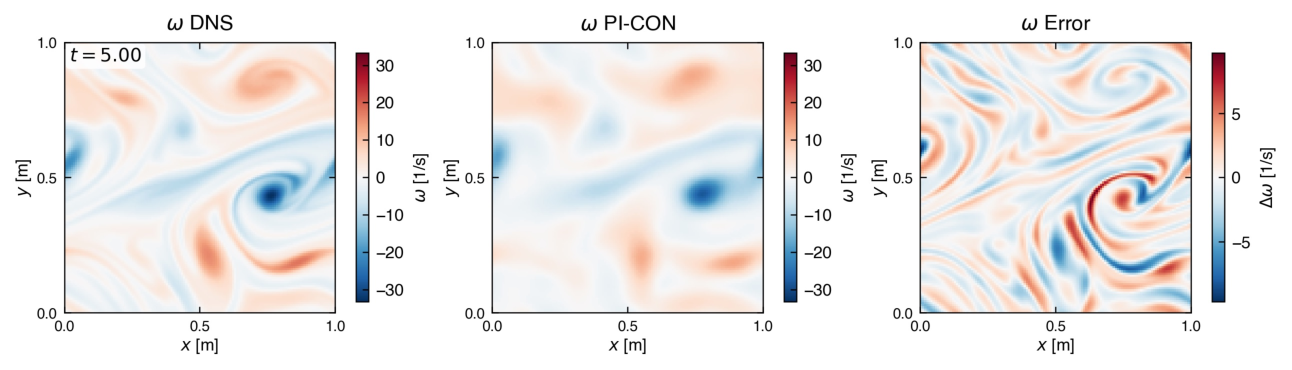
\includegraphics[width=0.92\linewidth]{figures/results/vorticity_comparison_t5.pdf}
    \caption{Vorticity fields at $t=5$ (seed 42). Left: DNS; middle: PI-CON prediction; right: error $\omega_{\rm pred} - \omega_{\rm DNS}$ (1/s). Axes: $x, y$ on $\Omega=[0,1]^2$ m$^2$. Left and middle share a colourbar; the error panel uses an independent symmetric scale.}
    \label{fig:vorticity_t5}
\end{figure}

Figure~\ref{fig:field_t5} compares $u$, $v$, and $\omega$ at $t=5$. PI-CON recovers the dominant DNS structures (large-scale shear bands in $u$ and energy-containing vortices in $v$) with the correct positions, signs, and amplitudes; residuals are fine-scale and structured rather than bulk offsets. The field is a low-pass reconstruction: energy-dominant large scales are recovered, while vorticity filaments and sharp cores are attenuated, matching the spectral roll-off in \S\ref{sec:spectrum}.

\paragraph{Discussion.}
The error structure in Figures~\ref{fig:field_t5}--\ref{fig:vorticity_t5} follows the $k^2$ amplification of $\omega$ relative to $u$ and $v$: vorticity is the hardest quantity to reconstruct under the $K=100$ budget and is reported as a diagnostic rather than a primary observable. The residual is spatially structured rather than random, pointing to a wavenumber-content limitation (\S\ref{sec:spectrum}). For engineering tasks driven by mean flow, kinetic energy, and dominant-structure positions, the $u$ and $v$ reconstruction in Figure~\ref{fig:field_t5} is adequate; tasks requiring fine-scale turbulence statistics (such as higher-order Reynolds-stress moments) need either more sensors or a different prior.

\paragraph{Low-order statistics.}
Beyond the instantaneous fields, the time- and span-averaged statistics quantify how well the reconstruction serves mean-flow monitoring. Figure~\ref{fig:mean_profile} reports the mean streamwise profile $\langle u\rangle_{x,t}(y)$ and the Reynolds shear stress $\langle u'v'\rangle_{x,t}(y)$, averaged over $x$ and the post-spin-up window $t\in[1,5]$~s. The mean profile agrees with DNS to $1.55\%$ relative $L_2$ error and the Reynolds shear stress to $8.61\%$; the two-lobe shear structure set by the $k_f=2$ forcing is reproduced in both amplitude and position. Low-order statistics fall well within the engineering target, supporting mean-flow and momentum-flux monitoring at the $K=100$ budget.

\begin{figure}[!htbp]
    \centering
    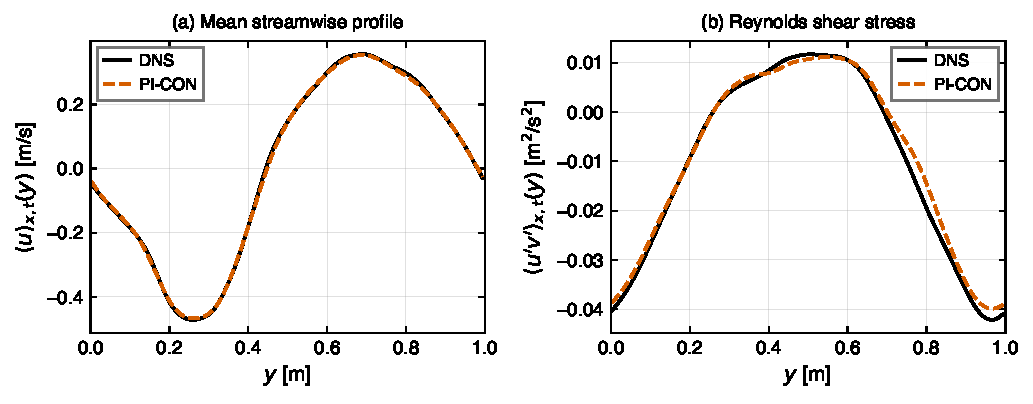
\includegraphics[width=\linewidth]{figures/results/mean_profile_reynolds.pdf}
    \caption{Low-order velocity statistics at $Re=10\,000$, $K=100$ (seed 42, LES-derived placement), averaged over $x$ and the window $t\in[1,5]$~s. (a) Mean streamwise profile $\langle u\rangle_{x,t}(y)$ (m/s) versus $y$ (m). (b) Reynolds shear stress $\langle u'v'\rangle_{x,t}(y)$ (m$^2$/s$^2$) versus $y$ (m). Solid: DNS; dashed: PI-CON.}
    \label{fig:mean_profile}
\end{figure}

\section{Spectral and Temporal Characterisation}
\label{sec:spectrum}

\paragraph{Energy spectrum evidence.}
\label{subsec:spectrum_evidence}

\begin{figure}[!htbp]
    \centering
    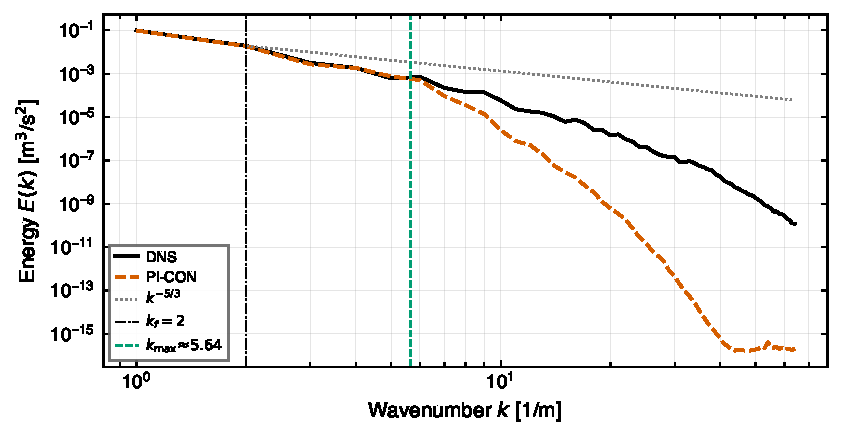
\includegraphics[width=0.92\linewidth]{figures/results/energy_spectrum.pdf}
    \caption{Radial energy spectrum at $t=5$ for the representative single seed (seed 42). Horizontal axis: wavenumber $k$ (1/m), log scale; vertical axis: radial energy spectrum $E(k)$ (m$^3$/s$^2$), log scale. DNS (solid black) and PI-CON prediction (dashed blue). Vertical dash-dotted line marks the forcing wavenumber $k_f = 2$; vertical dashed green line marks the sensor-count Nyquist scale $k_{\max}^{\rm sensor}\approx 5.64$.}
    \label{fig:spectrum}
\end{figure}

Figure~\ref{fig:spectrum} shows the radial energy spectrum at $t=5$. PI-CON matches the DNS spectrum within the sensor Nyquist band $k\le k_{\max}^{\rm sensor}\approx 5.64$ (carrying $\approx 99\%$ of the total energy at $t=5$); for $k\ge 16$ the prediction drops to a near-constant floor of $\approx 10^{-7}$, whereas the DNS continues a Kolmogorov-like cascade up to $k\sim 64$.

Figure~\ref{fig:band_err} reports the per-band relative error against time as the $n=5$ seed mean. The low band ($k\le 5$) decays over the window to a median of $2.5\%$ (range $0.07$--$14.9\%$ for $t>0$) and reaches near-zero at several instants. For $t\ge 0.5$\,s the high band ($k>16$) holds a median of $99.9\%$ (range $99.1$--$100.0\%$), the level a band carries when the reconstruction places no energy in it, while the mid band ($5<k\le 16$) holds a median of $53.5\%$ (range $41.7$--$71.0\%$). (The $t=0$ frame is excluded because high-$k$ energy there is near-zero, making relative error singular.)

\paragraph{Discussion.}
The high-$k$ deviation is the expected signature of a sensor-limited reconstruction rather than a model defect. At $K=100$ the available measurements constrain the energy-dominant low-wavenumber band but do not independently determine the mid and high bands. The $K$-scaling experiment in \S\ref{subsec:nyquist_scaling} provides further evidence: the reconstruction bandwidth tracks the sensor-count Nyquist scale.

\begin{figure}[!htbp]
    \centering
    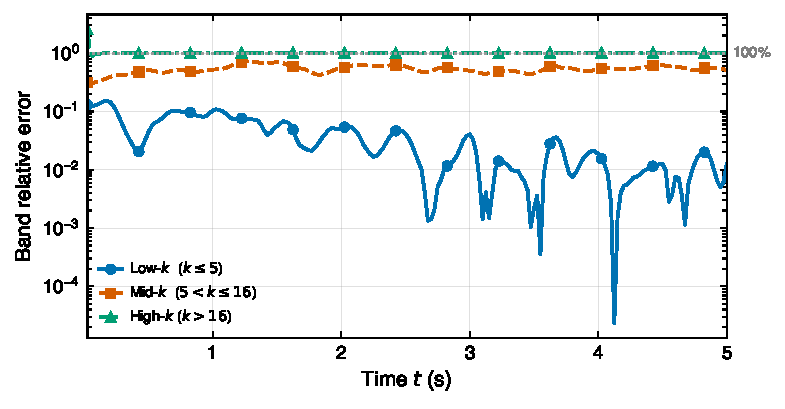
\includegraphics[width=0.85\linewidth]{figures/results/band_energy_rel_error_vs_time.pdf}
    \caption{Band-energy relative error (dimensionless) vs.\ time $t$ (s), LES-derived placement. Mean (solid, markers) $\pm 1\sigma$ (shaded) over $n=5$ seeds, with individual seeds dotted. Bands: low-$k$ ($k\le 5$, sensor-count Nyquist scale), mid-$k$ ($5<k\le 16$), high-$k$ ($k>16$). The $t=0$ frame is excluded.}
    \label{fig:band_err}
\end{figure}

\paragraph{Enstrophy and dissipation under the spectral cutoff.}
The band-limited reconstruction carries a direct consequence for vorticity-derived statistics. Figure~\ref{fig:dissipation_budget} compares the enstrophy $\mathcal{Z}(t)$ against DNS, with the dissipation rate $\varepsilon=2\nu\mathcal{Z}$ on the right axis as a constant rescaling. The reconstruction lies below the DNS reference by $26.0 \pm 0.2\%$ ($n=5$ seeds) on the post-spin-up window $t\ge 1$~s, because the mid/high-wavenumber content beyond the $K=100$ Nyquist scale carries enstrophy weighted by $k^2$. The deficit follows the spectral roll-off at $k\ge 16$ (Fig.~\ref{fig:spectrum}) and the $\omega$ relative error of Table~\ref{tab:main_metrics}: kinetic energy, concentrated at low wavenumbers, is recovered, while enstrophy-level statistics remain sensor-bounded.

\begin{figure}[!htbp]
    \centering
    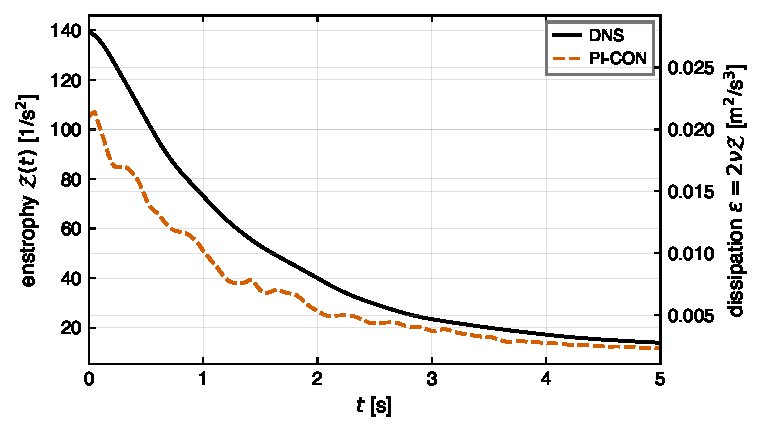
\includegraphics[width=\linewidth]{figures/results/dissipation_budget.pdf}
    \caption{Enstrophy $\mathcal{Z}(t)$ (left axis, 1/s$^2$) versus time $t$ (s), LES-derived placement; the right axis shows the dissipation rate $\varepsilon=2\nu\mathcal{Z}$ (m$^2$/s$^3$), a constant rescaling of the left axis. Solid: DNS reference (identical across seeds). Dashed: PI-CON mean over $n=5$ seeds, with the $\pm 1\sigma$ band shaded and individual seeds dotted.}
    \label{fig:dissipation_budget}
\end{figure}

\paragraph{Forcing-mode ($k = k_f = 2$) diagnostic.}
Because $k_f = 2$ lies inside the sensor-resolvable low band, the forcing-mode amplitude and phase check the energy-injection scale. Over $n=5$ seeds, after the initial-condition window ($t\ge 1$~s), the amplitude ratio holds near unity (mean $0.99$) and the phase error stays within $0.09$~rad ($\approx 5^\circ$), ending at $-0.013$~rad (Fig.~\ref{fig:kf_mode}), recovering the forced response; broadband pointwise fidelity is reported separately in Table~\ref{tab:main_metrics}.

\begin{figure}[!htbp]
    \centering
    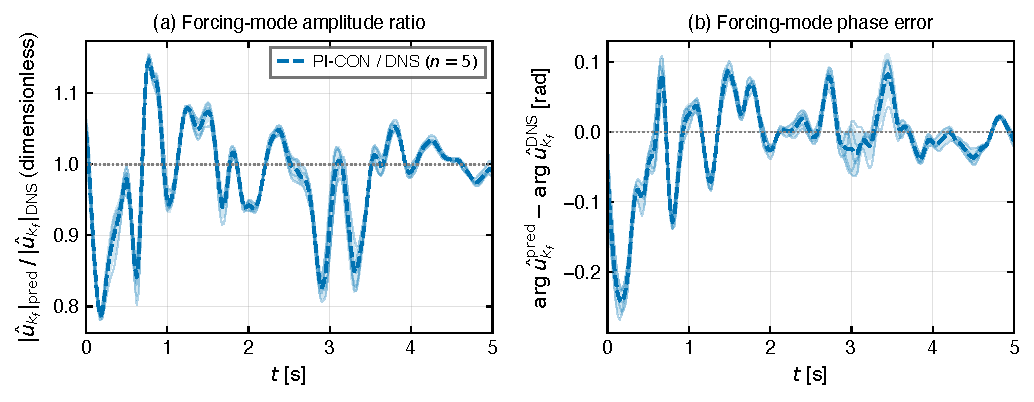
\includegraphics[width=\linewidth]{figures/results/kf_mode_diagnostic.pdf}
    \caption{Forcing-mode ($k_f = 2$) reconstruction over $n=5$ seeds, LES-derived placement. (a) Amplitude ratio $|\hat{u}_{k_f}|_{\rm pred}/|\hat{u}_{k_f}|_{\rm DNS}$ (dimensionless) versus time $t$ (s). (b) Phase error $\arg\hat{u}_{k_f}^{\rm pred}-\arg\hat{u}_{k_f}^{\rm DNS}$ (rad) versus $t$ (s). Dashed: across-seed mean; dotted: individual seeds; shaded: $\pm 1\sigma$; dotted grey lines mark the ideal amplitude ratio $1$ and zero phase error.}
    \label{fig:kf_mode}
\end{figure}

\paragraph{Temporal dynamics.}
Because the CfC branch encodes the sensor time series rather than reconstructing each frame independently, the reconstruction is also assessed in the time domain. Figure~\ref{fig:temporal_consistency} shows a velocity probe trace at the domain centre and the spatially-averaged temporal autocorrelation $R_{uu}(\tau)$. The probe trace follows the DNS instantaneous evolution, and the autocorrelation reproduces the DNS decorrelation: the $1/e$ time is $0.40$~s for PI-CON against $0.375$~s for DNS. The reconstruction recovers the temporal decorrelation structure, not only per-frame spatial statistics. A forward LES initialised from the same field departs from the DNS over this window (Fig.~\ref{fig:temporal_consistency}a, dotted), so the instantaneous probe evolution is recovered from the sparse sensor stream, not from a forward simulation.

\begin{figure}[!htbp]
    \centering
    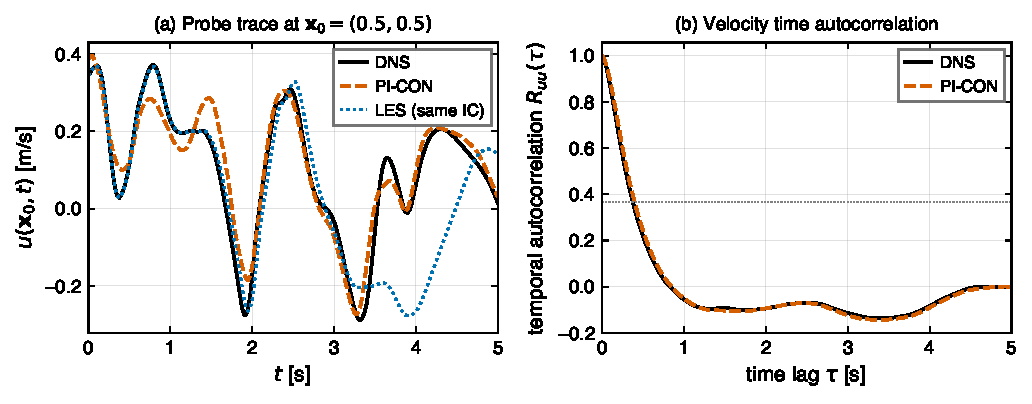
\includegraphics[width=\linewidth]{figures/results/temporal_consistency.pdf}
    \caption{Temporal behaviour at $Re=10\,000$, $K=100$ (seed 42, LES-derived placement). (a) Velocity probe trace $u(\mathbf{x}_0,t)$ (m/s) at the domain centre $\mathbf{x}_0=(0.5,0.5)$ versus $t$ (s); solid: DNS, dashed: PI-CON, dotted: a forward LES from the same initial field. (b) Spatially-averaged temporal autocorrelation $R_{uu}(\tau)$ (dimensionless) versus time lag $\tau$ (s) for DNS (solid) and PI-CON (dashed); the horizontal dotted line marks the $1/e$ level.}
    \label{fig:temporal_consistency}
\end{figure}

\section{Architectural Ablation}
\label{sec:supporting_comparisons}

This section attributes the main result to its components: a divergence diagnostic confirming the continuity constraint is active, then the $2\times2$ architecture ablation under the final PI-CON training protocol.

\paragraph{Divergence diagnostic.}
\label{sec:sub_dns_div}
The main pipeline applies Augmented-Lagrangian (AL) continuity at $\rho=0.1$, and the reconstructed field attains divergence ratio $0.39 \pm 0.006\%$ over $n=5$ seeds (Table~\ref{tab:main_metrics}): a physical-convergence check that the constraint is active, carrying no comparative meaning against DNS. The finite-difference operator is bandwidth-dependent: it registers $1.04\%$ on the full-cascade DNS field but $0.38\%$ once that field is band-limited to $k\le 16$ (\S\ref{subsec:dns_verification}); at matched bandwidth the reconstruction's $0.39\%$ sits at the $k\le 16$ DNS level, so the constraint drives divergence to the finite-difference floor permitted by its resolved scales rather than below DNS. The same recipe attains $0.37\%$ at $Re=10^{6}$, consistent across Reynolds numbers. The AL-strength sweep selecting $\rho=0.1$ is a hyperparameter diagnostic reported in Appendix~\ref{app:diagnostic_ablation_forward_cfd}.

\paragraph{Architectural ablation matrix.}
\label{sec:baseline_comparison}
The ablation isolates the contribution of CfC and cross-attention under the final common supervision regime. A $2\times2$ matrix toggles CfC and cross-attention independently: Vanilla DeepONet (B0), CfC-only (B1), Cross-attention-only (B2), and Full PI-CON (B3). The four cells share the supervision regime of \S\ref{sec:engineering_constraint}, the optimizer, the LES $T=50$ sensor placement, and $1024$ physics-collocation points used by the main pipeline (\S\ref{sec:main_result}). Engineering-transferable interpolation baselines (RBF, IDW, divergence-free trigonometric least squares) are compared against PI-CON in Appendix~\ref{app:fair_baselines}: PI-CON reduces pointwise $u$ rel-$L_2$ by $47$--$74\%$ relative to them despite their lower KE, which comes from over-smoothing toward the inter-sensor mean rather than better reconstruction.

\begin{table}[!htbp]
    \centering
    \caption{$2\times2$ architectural ablation at $Re=10\,000$, $K=100$, LES $T=50$ placement, $1024$ collocation points. All rows report mean $\pm$ standard deviation over $n=5$ seeds $\{42,1,2,3,4\}$ at $20\,000$ iterations. Relative-error metrics are percentages.}
    \label{tab:ablation_22matrix}
    \footnotesize
    \setlength{\tabcolsep}{3pt}
    \begin{tabularx}{\textwidth}{
        >{\raggedright\arraybackslash}p{4.0cm}
        >{\centering\arraybackslash}X
        >{\centering\arraybackslash}X
        >{\centering\arraybackslash}X
        >{\centering\arraybackslash}X
        >{\centering\arraybackslash}p{1.3cm}
    }
    \toprule
    \textbf{Variant} & \textbf{$u$ $L_2$ \%} & \textbf{$v$ $L_2$ \%} & \textbf{$\omega$ $L_2$ \%} & \textbf{KE \%} & \textbf{Params} \\
    \midrule
    B0 Vanilla DeepONet     & $15.42 {\pm} 0.11$ & $20.28 {\pm} 0.12$ & $45.44 {\pm} 0.26$ & $8.23 {\pm} 0.22$ & $1.28$\,M \\
    B1 CfC only             & $18.05 {\pm} 0.14$ & $24.26 {\pm} 0.30$ & $51.14 {\pm} 0.31$ & $9.23 {\pm} 0.51$ & $3.14$\,M \\
    B2 Cross-attention only & $14.64 {\pm} 0.12$ & $19.39 {\pm} 0.09$ & $44.32 {\pm} 0.17$ & $7.03 {\pm} 0.14$ & $2.74$\,M \\
    B3 Full PI-CON (Ours)   & $\mathbf{13.65 {\pm} 0.06}$ & $\mathbf{17.52 {\pm} 0.10}$ & $\mathbf{41.79 {\pm} 0.12}$ & $\mathbf{5.71 {\pm} 0.11}$ & $3.14$\,M \\
    \bottomrule
    \end{tabularx}
\end{table}

\paragraph{Architectural ranking under the main pipeline.}
With all four cells trained at the matched $20\,000$-iteration, $n=5$-seed budget, the KE ordering is B3 ($5.71 \pm 0.11\%$) $\prec$ B2 ($7.03 \pm 0.14\%$) $\prec$ B0 ($8.23 \pm 0.22\%$) $\prec$ B1 ($9.23 \pm 0.51\%$). Seed-paired Welch $t$-tests confirm every gap to B3 is significant: $-2.52$ percentage points versus B0 ($t=22.9$, $p=3.0\times10^{-7}$), $-3.52$ versus B1 ($t=15.1$, $p=5.5\times10^{-5}$), and $-1.32$ versus B2 ($t=16.3$, $p=2.4\times10^{-7}$). Decomposing the $2\times2$ on the absolute KE scale about the B0 reference cell (where the decomposition is additive) separates a cross-attention main effect of $-1.20$ percentage points, a CfC main effect of $+1.00$, and a CfC$\times$cross-attention interaction of $-2.32$, summing to the $-2.52$ B3$-$B0 total. Cross-attention is the dominant lever. CfC raises KE error on its own (mean-pool aggregation in B1 erodes the per-query specificity that physics-residual sampling supplies) but carries a large negative interaction, so it lowers error only in combination with the cross-attention readout.

\section{Sensing-Configuration Study}
\label{sec:sensing_study}

Three sensing-configuration levers govern reconstruction quality: sensor count, placement, and measurement noise. This section quantifies the sensor count and its Nyquist scale, then reports placement and noise robustness.

\subsection{Nyquist-Aligned K-Scaling}
\label{subsec:nyquist_scaling}

The most direct test of the information-limited interpretation varies sensor count while keeping the LES-derived placement principle fixed. For point sensors on a two-dimensional domain, the sensor-count Nyquist estimate gives
\begin{equation}
    k_{\max}^{\rm sensor} \;\approx\; \sqrt{K/\pi},
\end{equation}
a scale for the reconstructable band rather than a hard cutoff. It counts each sensor as a single sample, whereas the two measured velocity components $(u,v)$ at the divergence-free-constrained locations push the strict linear-observability limit somewhat higher (for $K=100$ the sensing matrix stays full-rank up to $k\lesssim 8$, Appendix~\ref{app:info_ceiling_diagnostics}). Raising $K$ from $100$ to $200$ and $400$ moves this scale from $\approx 5.64$ to $7.98$ and $11.28$.

Read against the DNS energy distribution, the scale locates how much energy lies within reach of each sensor count. Figure~\ref{fig:nyquist_recoverability} integrates the DNS energy CDF at $t=5$ over the $|\mathbf{k}|\le k_{\max}^{\rm sensor}$ disk, giving $98.9\%$, $99.7\%$, and $99.9\%$ of total kinetic energy at $K=100$, $200$, and $400$. These fractions report the energy available below the sensor-count scale, not a proof that higher-$k$ energy is unrecoverable. The information-limited reading rests instead on the empirical cutoff tracking $\sqrt{K/\pi}$ as $K$ grows.

\begin{figure}[!htbp]
    \centering
    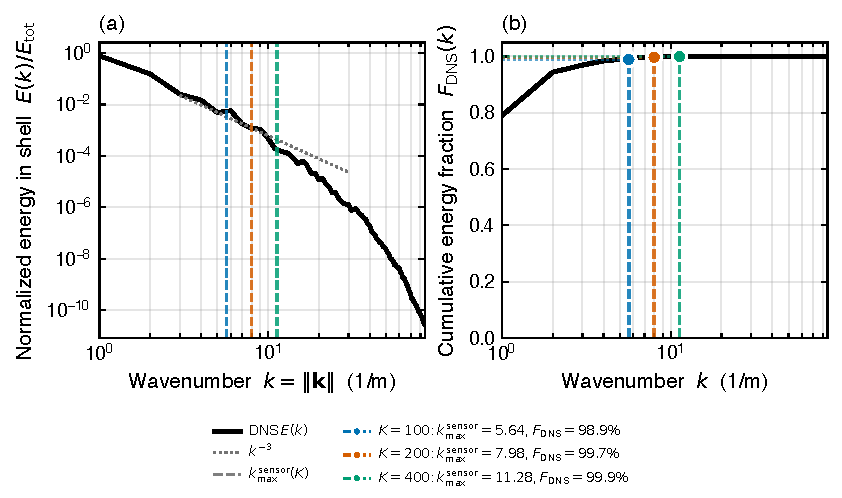
\includegraphics[width=0.95\linewidth]{figures/results/nyquist_recoverability.pdf}
    \caption{DNS energy available within the sensor-count Nyquist scale $\sqrt{K/\pi}$ for $K$ point velocity sensors ($Re=10^4$, $N=256$, $t=5$~s). (a)~Radial DNS energy spectrum $E(k)/E_{\rm tot}$ (dimensionless) versus wavenumber $k$ (1/m), with the $k^{-3}$ enstrophy-cascade reference (dotted; the forward-cascade slope for $k>k_f$) and Nyquist scales $k_{\max}^{\rm sensor}=\sqrt{K/\pi}$ (vertical dashed, colour-coded by $K$). (b)~Cumulative DNS energy fraction $F_{\rm DNS}(k)$ (dimensionless) versus $k$ (1/m); markers locate $F_{\rm DNS}(k_{\max}^{\rm sensor})$ for $K\in\{100,200,400\}$.}
    \label{fig:nyquist_recoverability}
\end{figure}

Table~\ref{tab:k_scaling_nyquist} reports the empirical reconstruction following this Nyquist-predicted bandwidth expansion.

\begin{table}[!htbp]
    \centering
    \caption{Sensor-count scaling against the Nyquist scale $\sqrt{K/\pi}$. LES-derived QR-pivot sensors, seed 42, $20\,000$ iterations; metrics at $t=5$. The $K=400$ run uses $512$ collocation points (memory budget).}
    \label{tab:k_scaling_nyquist}
    \small
    \setlength{\tabcolsep}{5pt}
    \begin{tabular}{lccc}
    \toprule
    \textbf{Quantity} & \textbf{$K=100$} & \textbf{$K=200$} & \textbf{$K=400$} \\
    \midrule
    Nyquist $k_{\max}^{\rm sensor}$ & 5.64 & 7.98 & 11.28 \\
    KE MAPE & 5.90\% & 2.47\% & \textbf{1.76\%} \\
    $u$ rel-$L_2$ & 7.10\% & 4.95\% & 4.11\% \\
    $v$ rel-$L_2$ & 16.08\% & 10.30\% & 8.64\% \\
    $\omega$ rel-$L_2$ & 38.03\% & 31.36\% & 29.29\% \\
    $k_f$ amplitude ratio & 0.969 & \textbf{0.998} & 0.975 \\
    \bottomrule
    \end{tabular}
\end{table}

\begin{figure}[!htbp]
    \centering
    \begin{subfigure}[t]{0.32\linewidth}
        \centering
        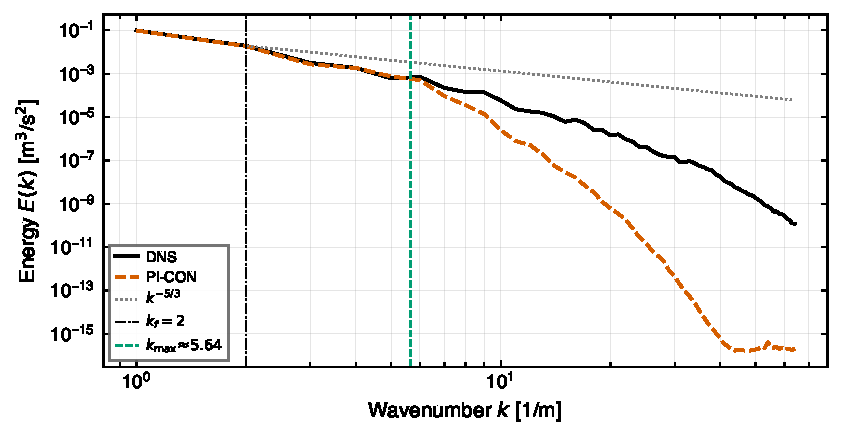
\includegraphics[width=\linewidth]{figures/results/spectrum_K100_nyquist.pdf}
        \caption{$K=100$, $k_{\max}^{\rm sensor}\approx 5.64$}
        \label{fig:spectrum_K100}
    \end{subfigure}\hfill
    \begin{subfigure}[t]{0.32\linewidth}
        \centering
        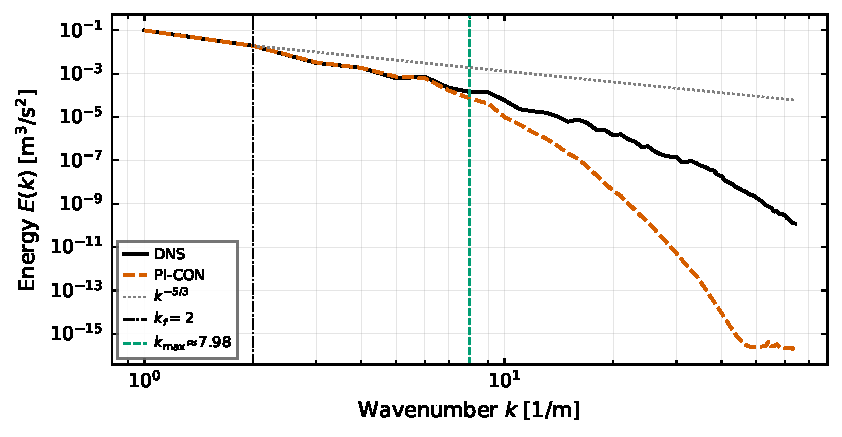
\includegraphics[width=\linewidth]{figures/results/spectrum_K200_nyquist.pdf}
        \caption{$K=200$, $k_{\max}^{\rm sensor}\approx 7.98$}
        \label{fig:spectrum_K200}
    \end{subfigure}\hfill
    \begin{subfigure}[t]{0.32\linewidth}
        \centering
        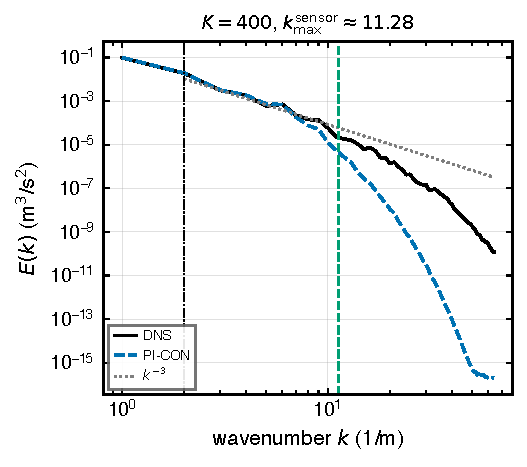
\includegraphics[width=\linewidth]{figures/results/spectrum_K400_nyquist.pdf}
        \caption{$K=400$, $k_{\max}^{\rm sensor}\approx 11.28$}
        \label{fig:spectrum_K400}
    \end{subfigure}
    \caption{Radial energy spectrum $E(k)$ (m$^3$/s$^2$) versus wavenumber $k$ (1/m) at $t=5$ for three sensor budgets. Each panel: DNS (solid black), PI-CON (dashed blue), $k^{-3}$ enstrophy-cascade reference (dotted grey; the forward-cascade slope for $k>k_f$), forcing $k_f = 2$ (dash-dotted black), sensor Nyquist $k_{\max}^{\rm sensor}=\sqrt{K/\pi}$ (dashed green). LES-derived QR-pivot, seed $42$, $20\,000$ iterations.}
    \label{fig:k_scaling_spectra}
\end{figure}

The agreement is qualitative but clear: at $K=100$ the $\sqrt{K/\pi}$ scale sits near the low/mid-band boundary, $K=200$ pushes it close to $k\approx 8$, and $K=400$ reaches into the inertial-range content (Figure~\ref{fig:k_scaling_spectra}). KE error drops by $70\%$ between $K=100$ and $K=400$ ($5.90\%\to1.76\%$; the $K=100$ value is the seed-42 single run, whose $n=5$ mean is $5.71\%$, Table~\ref{tab:multiseed}). The observed KE ratios relative to $K=100$ are $0.42$ at $K=200$ and $0.30$ at $K=400$. The Nyquist relation $k_{\max}^{\rm sensor}\propto\sqrt{K}$, under which the unresolved energy above the cutoff scales as $k_{\max}^{-2}\propto 1/K$, predicts ratios of $100/K = 0.50$ and $0.25$ respectively, placing the measured curve within $20\%$ of this scaling estimate. Because the $K=400$ run uses fewer collocation points, the three-point curve should not be read as a strict fit; it shows that higher fidelity comes from sensor bandwidth expansion, not from architecture search.


\subsection{Information-Ceiling Summary}
\label{sec:info_limit_summary}

The $K=100$ result should be read against the sensor information ceiling rather than as an unconstrained full-field regression problem. A wavelet sparsity diagnostic, a sensing-matrix rank calculation, and a spectral-truncation bound point to the same interpretation: the low-wavenumber band is observable enough to support engineering KE and mean-flow monitoring, while mid- and high-wavenumber content remains underdetermined at this sensor budget. The B3 multi-seed KE error ($5.71\%$) maps to an effective spectral cutoff $k_{\rm cut}\approx 4.7$ and the $k^2$-weighted vorticity error to $k_{\rm cut}\approx 7.8$ (Appendix~\ref{app:info_ceiling_diagnostics}); the two bracket the sensor Nyquist estimate $k_{\max}^{\rm sensor}\approx 5.64$, as the sensor-count criterion of \S\ref{sec:research_questions} requires. Closing the remaining mid/high-band error therefore requires more sensors or extra modalities, not another architecture-side loss term.

The detailed wavelet, SVD, and spectral-truncation diagnostics are collected in Appendix~\ref{app:info_ceiling_diagnostics}.

\subsection{Sensor Placement Analysis}
\label{sec:placement_analysis}

Placement strategy contributes a variance source larger than training stochasticity at fixed $K=100$. Table~\ref{tab:placement_strategy_new} summarises the final-protocol placement comparison: DNS-oracle and LES-derived placements differ only in sensor-placement source and are both trained over $n=5$ random seeds at $20\,000$ iterations (Table~\ref{tab:main_metrics}); random placement is repeated over $n=5$ placement seeds with training seed fixed to isolate placement variance.

\begin{table}[!htbp]
    \centering
    \caption{Final-protocol placement comparison at $Re=10\,000$, $K=100$, B3, $1024$ collocation points, $20\,000$ iterations. DNS-oracle and LES-derived placements report training-seed mean $\pm$ standard deviation. Random placement reports placement-seed mean $\pm$ standard deviation with training seed fixed at $42$. In all rows the sensor \emph{values} are read from the DNS field that stands in for the real-world flow (at the $K$ sensor positions only); the second column marks only whether \emph{placement} additionally requires the DNS \emph{full field}.}
    \label{tab:placement_strategy_new}
    \footnotesize
    \setlength{\tabcolsep}{3pt}
    \begin{tabularx}{\textwidth}{
        >{\raggedright\arraybackslash}p{3.4cm}
        >{\centering\arraybackslash}X
        >{\centering\arraybackslash}X
        >{\centering\arraybackslash}X
        >{\centering\arraybackslash}X
    }
    \toprule
    \textbf{Placement strategy} & \textbf{DNS \emph{full field} for placement?} & \textbf{KE \%} & \textbf{$u$ $L_2$ \%} & \textbf{Interpretation} \\
    \midrule
    DNS QR-pivot oracle & Yes & $\mathbf{4.68 \pm 0.06}$ & $15.34 \pm 0.06$ & non-deployable lower-KE reference \\
    LES-derived QR-pivot & No & $5.71 \pm 0.11$ & $\mathbf{13.65 \pm 0.06}$ & main deployable placement \\
    Random uniform & No & $7.95 \pm 0.68$ & $17.20 \pm 1.42$ & no-placement-effort reference \\
    \bottomrule
    \end{tabularx}
\end{table}

\paragraph{Strategy comparison.}
All three strategies stay below the $10\%$ KE engineering target. The DNS oracle gives the lowest integral KE error ($4.68\%$), but the LES-derived placement gives lower pointwise velocity error ($u$ rel-$L_2$ $13.65\%$ vs.\ $15.34\%$) while needing no DNS full field to place the sensors. Random placement remains feasible ($7.95\%$ KE) but less reliable: placement changes reliability more than feasibility. The final pipeline adopts LES-derived QR-pivot placement as the deployable reference: it approaches the DNS oracle without needing a DNS full field for placement, and improves over random placement by $2.24$ KE percentage points.

\label{sec:placement_variance}

To estimate placement-induced variance separately from training stochasticity, the random-uniform strategy is repeated at $n=5$ placement seeds ($42, 1, 2, 3, 4$) with the training seed held at $42$.

\begin{table}[!htbp]
    \centering
    \caption{Random $K=100$ placement variance at $Re=10\,000$, B3, $1024$ collocation points, $20\,000$ iterations, training seed $42$. Each placement seed selects $K=100$ uniformly-random positions on the $256^2$ grid. Error columns: relative-error percentages (KE is MAPE); divergence ratio $= \Vert\nabla\!\cdot\!\mathbf{u}\Vert_2 / \Vert\nabla\mathbf{u}\Vert_F^{\rm DNS}$.}
    \label{tab:placement_variance}
    \footnotesize
    \setlength{\tabcolsep}{3pt}
    \begin{tabularx}{\textwidth}{
        >{\raggedright\arraybackslash}p{1.8cm}
        >{\centering\arraybackslash}X
        >{\centering\arraybackslash}X
        >{\centering\arraybackslash}X
        >{\centering\arraybackslash}X
        >{\centering\arraybackslash}X
    }
    \toprule
    \textbf{Placement seed} & \textbf{KE \%} & \textbf{$u$ $L_2$ \%} & \textbf{$v$ $L_2$ \%} & \textbf{div ratio \%} & \textbf{$k_f$ amp} \\
    \midrule
    $42$ & $7.24$            & $16.14$ & $20.33$ & $0.37$ & $\mathbf{1.001}$ \\
    $1$  & $\mathbf{9.18}$\,$^\dagger$ & $19.80$ & $25.64$ & $0.34$ & $0.941$ \\
    $2$  & $7.89$            & $16.48$ & $20.86$ & $0.36$ & $0.962$ \\
    $3$  & $8.03$            & $16.10$ & $20.16$ & $0.35$ & $0.966$ \\
    $4$  & $7.40$            & $17.47$ & $21.11$ & $0.34$ & $0.995$ \\
    \midrule
    \textbf{mean$\pm$std} & $\mathbf{7.95 {\pm} 0.68}$ & $17.20 {\pm} 1.42$ & $21.62 {\pm} 2.07$ & $\mathbf{0.35 {\pm} 0.01}$ & $0.973 {\pm} 0.024$ \\
    \bottomrule
    \end{tabularx}
    \\[2pt]
    \footnotesize $^\dagger$Outlier; random placement occasionally hits a configuration with poor spatial coverage.
\end{table}

\paragraph{Placement versus training variance.}
The two five-seed estimates yield $\sigma_{\rm training}=0.11\%$ (LES $T=50$, Table~\ref{tab:multiseed}) and $\sigma_{\rm placement}=0.68\%$ (random uniform, Table~\ref{tab:placement_variance}); placement variance dominates training stochasticity by
\begin{equation}
    \sigma_{\rm placement}/\sigma_{\rm training} \;\approx\; 6.2\times.
    \label{eq:placement_dominance}
\end{equation}
The ratio in \eqref{eq:placement_dominance} shows that LES-derived placement improves both the mean (KE $5.71\%$ vs.\ $7.95\%$, $\Delta=2.24$ percentage points, Welch $z \approx 3.3$, $p<0.01$) and the reproducibility ($6.2\times$ tighter), so engineering deployment should prioritise placement optimisation over training repetition. Divergence ratio stays at $0.35 \pm 0.01\%$ across all five placement seeds: the divergence diagnostic (\S\ref{sec:sub_dns_div}) is placement-invariant within the random-uniform family.

\paragraph{Field alignment does not improve placement.}
The placement LES is an independent, long-horizon realisation (\S\ref{sec:les_placement}). Initialising LES from the DNS field might seem preferable because it tracks the DNS pointwise for about one eddy-turnover time (Fig.~\ref{fig:les_predictability}), but Table~\ref{tab:placement_dnsinit} shows the opposite. A DNS-initialised LES integrated only to $t=5$ gives worse placement (KE $9.12\%$) than the long-horizon random-IC $T=50$ LES ($5.90\%$) at the same training seed. QR-pivot placement depends on leading POD modes, so a short DNS-seeded spin-down trajectory is less useful than a longer attractor sample. The dns-init run also requires a DNS field to seed and is diagnostic only.

\begin{table}[!htbp]
    \centering
    \caption{Field-aligned versus long-horizon sensor placement at $Re=10\,000$, $K=100$, B3, $1024$ collocation points, $20\,000$ iterations, single training seed $42$. The $t=5$ dns-init LES is initialised from the DNS field, so it tracks the DNS pointwise at early time, but it is a diagnostic (it needs a DNS field to seed), not a deployable option. KE is MAPE (percent); $\tau$ denotes the eddy-turnover time.}
    \label{tab:placement_dnsinit}
    \small
    \begin{tabular}{llc}
    \toprule
    \textbf{Placement source} & \textbf{POD window} & \textbf{KE \%} \\
    \midrule
    LES $T=50$, random IC (deployable)         & $\sim 22\,\tau$  & $5.90$ \\
    LES $t=5$, dns-init (field-aligned; diag.) & $\sim 2.5\,\tau$ & $9.12$ \\
    \bottomrule
    \end{tabular}
\end{table}

\subsection{Sensor Noise Robustness}
\label{sec:noise_robustness}

Because the main pipeline relies on measured sensor time series rather than full-field supervision, moderate observation noise must not dominate reconstruction. Table~\ref{tab:noise_robustness} reports the response to per-channel Gaussian noise at $1$--$10\%$ of the sensor standard deviation, with the LES-derived layout and final $20\,000$-iteration, $1024$-collocation training setup fixed. The sweep uses $n=5$ seeds at each noise level and supports O3 by testing whether the trained recipe remains within the engineering target under controlled additive perturbations.

\begin{table}[!htbp]
    \centering
    \caption{Sensor-noise robustness of the LES-pivot pipeline under the final PI-CON protocol ($20\,000$ iterations, $1024$ collocation, $n=5$ seeds per noise level). Noise level is relative to the per-channel sensor standard deviation; $\Delta$~KE is measured against the clean final-protocol baseline.}
    \label{tab:noise_robustness}
    \small
    \setlength{\tabcolsep}{5pt}
    \begin{tabular}{lccccc}
    \toprule
    \textbf{Noise $\sigma$} & \textbf{KE \%} & \textbf{$\Delta$ KE} & \textbf{$u$ $L_2$ \%} & \textbf{$v$ $L_2$ \%} & \textbf{div ratio \%} \\
    \midrule
    Clean & $5.71 {\pm} 0.11$ & -- & $13.65 {\pm} 0.06$ & $17.52 {\pm} 0.10$ & $0.39 {\pm} 0.006$ \\
    1\%  & $5.75 {\pm} 0.08$ & $+0.04$ & $13.66$ & $17.57$ & $0.40$ \\
    3\%  & $5.81 {\pm} 0.03$ & $+0.10$ & $13.74$ & $17.70$ & $0.40$ \\
    5\%  & $5.92 {\pm} 0.08$ & $+0.21$ & $13.90$ & $17.92$ & $0.42$ \\
    10\% & $6.08 {\pm} 0.21$ & $+0.37$ & $14.49$ & $18.77$ & $0.46$ \\
    \bottomrule
    \end{tabular}
\end{table}

The aggregate trend is monotone: increasing sensor noise raises KE error, pointwise error, vorticity error, and divergence ratio. Even at $10\%$ sensor noise, however, the KE error remains $6.08 \pm 0.21\%$, well below the $10\%$ engineering threshold. This supports the deployment criterion without relying on the older single-seed regularisation artefact.

\section{Higher-Reynolds Feasibility}
\label{sec:cross_reynolds}

The same architecture, with the sensor budget and model capacity retuned, is applied at $Re=10^{6}$ to probe whether the approach remains feasible two orders of magnitude higher in Reynolds number.

At higher Reynolds numbers the spatial under-sampling ratio $d/\delta_\omega$ (sensor spacing $d = L/\sqrt{K}$ relative to vorticity layer thickness $\delta_\omega \propto Re^{-1/2}$) is approximately $10\times$ more severe than at $Re=10^{4}$.
Three adaptations are applied: sensor count is raised to $K=200$; the LES proxy is run to $T_{\rm end}=50$~s ($26.5$ turnover times) for long-horizon placement (\S\ref{sec:les_placement}); and the model is widened to $d_\text{model}=384$ with $50\,000$ training steps.
All other hyperparameters follow the $Re=10^{4}$ baseline (Chapter~\ref{ch:experiments_setup}).

Results are in Table~\ref{tab:re1e6}. KE MAPE attains $6.10\%$, close to the $Re=10^{4}$ baseline level ($5.71 \pm 0.11\%$, Table~\ref{tab:main_metrics}) but not directly comparable as a seed-statistics claim because the $Re=10^{6}$ run is single-seed and uses a retuned sensor budget, width, and step count. This is a feasibility case at higher Reynolds number, not a like-for-like generalisation or recipe-transfer claim.
The divergence diagnostic is consistent across Reynolds numbers: div-ratio $0.37\%$ matches the $Re=10^{4}$ value of $0.39\%$ (\S\ref{sec:sub_dns_div}), indicating the continuity constraint reaches its band-limited floor at both $Re$.
The forcing-mode amplitude ratio reaches $1.04$, confirming recovery of the dominant energy-injection mode.
Enstrophy rel-err ($42\%$) is higher than at $Re=10^{4}$, consistent with the wider gap between the sensor-count Nyquist scale ($k_\text{max}\approx8$ at $K=200$) and the $Re=10^{6}$ dissipation cut-off ($k\approx100$), rather than an architectural limitation.

\begin{table}[!htbp]
    \centering
    \caption{PI-CON at $Re=10^{6}$ with $K=200$, LES $T=50$ proxy placement, $d_\text{model}=384$, 50\,000 steps.}
    \label{tab:re1e6}
    \small
    \begin{tabular}{lc}
    \toprule
    \textbf{Metric} & \textbf{Value} \\
    \midrule
    KE MAPE & $6.10\%$ \\
    $u$ rel-$L_2$ & $15.62\%$ \\
    Enstrophy rel-err & $42.06\%$ \\
    Divergence ratio & $0.37\%$ \\
    $E(k_f)$ amplitude ratio & $1.04$ \\
    \bottomrule
    \end{tabular}
\end{table}

\paragraph{Comparison boundary.}
This is a single-seed feasibility check; multi-seed confirmation at $Re=10^{6}$ remains an open follow-up.
The key result is that matched low-frequency accuracy (KE $6.10\%$ vs.\ $5.71\%$) is achievable at $Re=10^{6}$ by scaling the sensor budget to the spatial under-sampling severity.


\paragraph{Diagnostic boundaries.}
Several diagnostic findings define the boundary of the final recipe without changing the main result. The Kolmogorov forcing parameters are not recovered from $K=100$ sensors under the tested setup (near-zero flat-region initialisation): accurate velocity reconstruction did not certify recovery of $A$ or $k_f$, though structural identifiability is not established. Extending Augmented-Lagrangian enforcement from continuity to the Navier--Stokes momentum residual is not promoted as a main-recipe improvement: the final-protocol rerun gives mixed single-seed results, so the final pipeline keeps the $n=5$-validated continuity-only AL recipe and leaves momentum residuals to GradNorm weighting. These functional-parameter and recipe diagnostics are reported in Appendix~\ref{app:diagnostic_ablation_forward_cfd} rather than used as Chapter~\ref{ch:results} evidence.

\section{Engineering Applicability}
\label{sec:engineering_app}

Inference cost is quantified below.

\paragraph{End-to-end pipeline cost.}
Table~\ref{tab:inference_cost} reports the end-to-end pipeline cost. The encoder pass costs $70.7 \pm 3.8$\,ms once per trajectory; subsequent spatial queries cost $32\,\mu$s per grid point ($31\,030$ queries/s). Because the trunk evaluates any coordinate directly, the operator answers an arbitrary space--time query without re-integrating the solver from an initial condition, meeting the query-anywhere requirement of O1 (\S\ref{sec:research_questions}). Sparse monitoring (up to $\sim 3\,000$ query points) completes within $100$\,ms, whereas a full $128^2$ field query costs $527.8 \pm 17.1$\,ms. Single-shot real-time full-field reconstruction on CPU or MPS therefore requires GPU or batched optimisation.

The one-time setup couples the placement-LES forward solve over the reconstruction window ($256^2$, $50\,000$ steps at $\Delta t = 10^{-4}$~s, $7.6$\,min) with operator training ($1.33$\,h), totalling $\approx 1.46$\,h against the $3.27$\,h required to solve the $1024^2$ DNS reference over the same window. The trained operator then reconstructs a full trajectory in $9.7$\,min against the $3.27$\,h DNS solve, a $20\times$ margin that meets the $\ge 5\times$ reconstruction-speed criterion of \S\ref{sec:research_questions}, and answers further space--time queries at negligible marginal cost, so the setup amortises across queries. Both margins mix hardware (GPU training and MPS inference against the CPU DNS solve) and are not the engineering case for the operator: forward simulation cannot reconstruct a field from sparse observations, and the DNS is unavailable on a new scene. The margin widens where a single high-fidelity solve is far more expensive (3D, multi-physics, or higher-Reynolds flows); establishing this remains an open follow-up.

\begin{table}[!htbp]
    \centering
    \caption{End-to-end cost of the PI-CON pipeline against the DNS reference. The one-time setup couples the placement-LES forward solve over the reconstruction window $t\in[0,5]$~s with operator training; per-trajectory inference is then reused for arbitrary space--time queries. Wall-clock is single-host CPU (numpy) for the LES and DNS solves, a single GPU for training, and Apple M3 MPS for inference, so the setup-versus-DNS ratio mixes hardware. Times in milliseconds (ms), minutes (min), or hours (h) as indicated; throughput in queries per second (q/s).}
    \label{tab:inference_cost}
    \small
    \setlength{\tabcolsep}{5pt}
    \begin{tabular}{llrl}
    \toprule
    \textbf{Stage} & \textbf{Configuration} & \textbf{Wall-clock} & \textbf{Hardware} \\
    \midrule
    \multicolumn{4}{@{}l}{\emph{One-time pipeline setup}} \\
    LES simulation        & $256^2$, $50\,000$ steps ($\Delta t = 10^{-4}$) & $7.6$\,min          & CPU (numpy) \\
    Operator training     & $20\,000$ steps                 & $1.33$\,h           & $1\times$ GPU \\
    \quad Setup subtotal  & LES $+$ training                & $\approx 1.46$\,h   & \\
    \midrule
    \multicolumn{4}{@{}l}{\emph{Per-trajectory inference}} \\
    Encode (sensor series)       & $T=201$, $K=100$ ($n=20$)    & $70.7 \pm 3.8$\,ms   & M3 MPS \\
    Field query                  & $16\,384$ pts/batch ($n=30$) & $527.8 \pm 17.1$\,ms & M3 MPS \\
    \quad (throughput)           &                              & $31\,030$\,q/s       & \\
    Full-sequence reconstruction & $603$ fields, $128^2$        & $9.7$\,min           & M3 MPS \\
    \midrule
    \multicolumn{4}{@{}l}{\emph{Reference}} \\
    DNS solve             & $1024^2$, $20\,000$ steps       & $3.27$\,h           & CPU (numpy) \\
    \midrule
    \textbf{Setup vs DNS solve} & LES $+$ training vs $1024^2$ DNS & $1.46$ vs $3.27$\,h & $\approx 2.2\times$ lower \\
    \bottomrule
    \end{tabular}
\end{table}

Encode cost accounts for $\approx 0.06\%$ of the full-sequence reconstruction time: encode once, then query any spatial point at negligible marginal cost.

\chapter{Conclusion}
\label{ch:discussion_conclusion}

\section{Summary}
\label{sec:summary}

This work reconstructed turbulent flow fields from sparse point sensors without full-field DNS supervision. PI-CON combines a CfC-DeepONet backbone, isotropic relative-position cross-attention, and an Augmented-Lagrangian-style continuity penalty. On 2D Kolmogorov at $Re=10\,000$ with $K=100$ sensors, it meets the engineering targets across DNS-oracle, DNS-free LES-derived, geometric space-filling, and random placement. LES-derived QR-pivoting is recommended as an informed DNS-free option because it improves over random placement in the evaluated setting, not because it is universally optimal: space-filling and the DNS oracle give lower KE error, whereas LES-derived placement gives lower pointwise error (Table~\ref{tab:placement_strategy_new}).

The three engineering success criteria of \S\ref{sec:research_questions} are met:
\begin{itemize}
    \item \textbf{(O1) An accurate and fast reconstructor.} The energy-dominant low-wavenumber band reaches single-digit relative error within the $10\%$ target (Fig.~\ref{fig:band_err}), with a $2\times2$ ablation confirming the architectural components under the final PI-CON protocol; once trained, the operator answers any space--time query in a single forward pass and reconstructs a full trajectory $20\times$ faster than re-solving the reference DNS on the hardware reported, meeting the $\ge 5\times$ criterion (Table~\ref{tab:inference_cost}), though a single full-field query is not real-time on CPU or MPS in the current implementation.
    \item \textbf{(O2) Sensor count sets the achievable resolution.} A divergence-free SVD and a $K$-scaling sweep ($K\in\{100,200,400\}$) attribute residual mid/high-band error to sensor information capacity, with the kinetic-energy- and vorticity-derived cutoffs bracketing the sensor-count sampling band edge, identifying sensor-density scaling as the productive direction (\S\ref{sec:info_limit}).
    \item \textbf{(O3) Placement and noise set reliability.} Four placement strategies (DNS-oracle, DNS-free LES, geometric space-filling, and random) all keep KE error within the engineering target. LES-derived QR-pivoting improves over random placement and is therefore recommended as an informed DNS-free option, while the metric-dependent ranking precludes a universal best-placement claim. Placement contributes a variance source $6.4\times$ training stochasticity; additive sensor noise up to $10\%$ keeps the reconstruction within the target in the noise-stress test.
\end{itemize}

\paragraph{Contributions.}
\begin{enumerate}
    \item \textbf{PI-CON architecture for engineering sparse-sensor reconstruction.} Under sensor-only-with-physics supervision, PI-CON attains KE MAPE $5.71 \pm 0.12\%$ ($n=5$ seeds) from $K=100$ sensors at $Re=10\,000$ (Table~\ref{tab:main_metrics}) and reconstructs any query point without re-solving the governing equations. The matched $2\times2$ ablation identifies cross-attention as the dominant architectural lever, with CfC useful through its interaction with the query-conditional readout.
    \item \textbf{A systematic sensing-configuration study.} Sensor count, placement, and noise are separated experimentally. A divergence-free SVD and $K\in\{100,200,400\}$ sweep show that count sets resolution (Table~\ref{tab:k_scaling_nyquist}); placement sets reliability, with placement variance $6.4\times$ training stochasticity and no single strategy dominating all metrics (Table~\ref{tab:placement_strategy_new}); and additive noise up to $10\%$ leaves reconstruction within the target. Sensor-density scaling, not architecture, is the productive direction for higher fidelity.
    \item \textbf{Cross-Reynolds feasibility under a single architecture.} At $Re=10^6$ with $K=200$ sensors the same architecture--AL recipe attains KE MAPE $6.10\%$ (Table~\ref{tab:re1e6}), showing feasibility over two orders of magnitude in Reynolds number. The result is single-seed and should be treated as an extension, not a multi-seed benchmark.
\end{enumerate}

\section{Engineering Implications}
\label{sec:engineering_impl}

Five implications follow:

\begin{itemize}
    \item \textbf{Energy-dominant band suffices for engineering use.} The low-wavenumber band is reconstructed at single-digit relative error from a DNS-free LES-pivot pipeline, sufficient for KE-based control, mean-flow monitoring, and phase-locked actuation.
    \item \textbf{Mid/high-band saturation has a quantified bound.} The near-$100\%$ higher-band error tracks the sensor-information limit, and $K$-scaling shows the effective bandwidth expanding with the predicted $\sqrt{K}$ scaling (\S\ref{sec:info_limit}).
    \item \textbf{Active incompressibility constraint across Reynolds numbers.} The Augmented-Lagrangian continuity constraint drives the reconstruction's divergence to the finite-difference floor of its resolved bandwidth at both reported Reynolds numbers (\S\ref{sec:sub_dns_div}), with no configuration switching required. Incompressibility-sensitive downstream tasks should validate against their own tolerance, since the reconstruction is band-limited near the sensor-count sampling band edge.
    \item \textbf{Streaming-friendly deployment.} Filtering mode reads no future sensors and the CfC formulation decouples query rate from sensor sampling; training uses no DNS full field, so deployment requires only the sensor stream.
    \item \textbf{Bounded sensitivity to observation noise.} Across the tested additive-noise range, KE remains below the $10\%$ engineering threshold, supporting robustness to modest observation noise while leaving realistic sensor-error models open.
\end{itemize}

\section{Limitations}
\label{sec:limitations}

\begin{itemize}
    \item \textbf{Observation noise.} The $1$--$10\%$ Gaussian noise sweep uses the final PI-CON protocol with $n=5$ seeds per noise level, but it still covers only additive per-channel Gaussian perturbations and excludes sensor-specific bias, drift, dropout, correlated channel noise, and calibration errors.
    \item \textbf{Geometry scope.} The main study uses a simple, obstacle-free, doubly periodic two-dimensional domain. A single non-periodic case (a cylinder wake with an explicit inflow boundary-condition loss) is validated as a preliminary extension in Appendix~\ref{app:cylinder}, but a systematic treatment of wall-bounded and obstacle-laden geometries (airfoil, internal flow) remains open.
    \item \textbf{Dimensionality.} All reported results are two-dimensional. Two-dimensional turbulence carries an inverse energy cascade and no vortex stretching, so the spectral content the reconstruction must recover differs in kind from three-dimensional turbulence. The sensor-information analysis of \S\ref{sec:info_limit} is likewise derived for a two-dimensional divergence-free basis, and its scaling does not transfer to three dimensions without rederivation.
    \item \textbf{Pressure field.} Only the velocity components $(u,v)$ are reconstructed under supervision. Pressure appears as a model-internal variable coupled to the loss solely through $\nabla p$ in the momentum residual, leaving both an additive gauge and the pressure magnitude underdetermined. The resulting internal pressure departs from the DNS reference in both gradient and gauge-removed value, and the departure is independent of the AL recipe (Appendix~\ref{app:pressure_limit}). Pressure-derived quantities --- surface loading, cavitation margin, and aeroacoustic source terms --- are therefore outside the validated scope.
    \item \textbf{Forcing form.} A single sustained body force $f_x = A\sin(2\pi k_f y)$ is used throughout. The architecture is forcing-agnostic, but wall-driven channel flow and inflow-driven wakes/jets require case-by-case revalidation.
    \item \textbf{Temporal sampling.} The CfC branch is adopted because a deployable temporal model must tolerate the irregular, unsynchronised timestamps of field sensors (\S\ref{subsec:cfc_encoder}), yet the controlled Kolmogorov benchmark samples uniformly at $0.025$~s. The irregular-clock capability is therefore carried by the formulation rather than exercised by the evidence reported here, and the $2\times2$ ablation (\S\ref{sec:baseline_comparison}) measures the CfC branch only on a fixed clock, where the time gap entering the cell is constant; this is the regime in which the branch is least able to pay for its aggregation cost. Whether the capability holds under non-uniform timestamps remains an open follow-up (\S\ref{sec:future_work}).
    \item \textbf{Acceptance metrics.} Primary KE, $u/v$ relative $L_2$, divergence, mean-profile, Reynolds-shear-stress, and enstrophy/dissipation diagnostics are covered; higher-order Reynolds-stress moments and full turbulent-kinetic-energy budget closure are not.
    \item \textbf{Per-case fitting and single-seed cross-$Re$.} PI-CON is fit once per case by design because high-Reynolds chaos ties each realisation to its conditions. Cross-case generality is not demonstrated, and the $Re=10^6$ extension is single-seed with unquantified seed variance.
    \item \textbf{CFD-rigour gaps.} The DNS passes Pope-2000 ($k_{\max}\eta=1.91$) but $T/t_{\rm eddy}=2.51$ gives a short statistical window.
    \item \textbf{Diagnostic boundaries.} Forcing parameters ($A$, $k_f$) were not recovered at $K=100$ sensors under the tested initialisation despite accurate reconstruction (\S\ref{sec:forcing_identifiability}); structural identifiability is not established. Multi-constraint AL remains a recipe diagnostic rather than a main conclusion: the final-protocol rerun gives mixed single-seed results, so the thesis keeps the continuity-only AL recipe, supported by the $n=5$ main baseline (\S\ref{sec:multi_al_negative}).
\end{itemize}

\section{Future Work}
\label{sec:future_work}

Nine directions follow from the limitations:
\begin{enumerate}
    \item \textbf{Sensor-budget scaling beyond the current curve.} Extend the $K=100/200/400$ sweep with $K=50$ and a matched training budget at $K=400$ to stress-test the agreement between the sensor-count sampling band edge and the effective reconstruction bandwidth, and to separate sensor bandwidth from compute-budget compromises.
    \item \textbf{Cross-Reynolds multi-seed confirmation.} The $Re=10^6$ extension (Table~\ref{tab:re1e6}) is single-seed; an $n=3$ multi-seed run quantifies its seed variance against the $Re=10^4$ baseline. A higher-Reynolds test ($Re \ge 10^7$) and sensor-density scaling at $Re=10^6$ ($K=400$) extend the cross-$Re$ envelope.
    \item \textbf{Realistic sensor-error model.} Go beyond additive Gaussian noise to bias, drift, dropout, correlated channel noise, and calibration uncertainty; assess whether sensor denoising or mean-enforced losses such as that of Mo and Magri~\cite{Mo2025PRF} are needed.
    \item \textbf{Irregular-clock validation.} Re-run the reconstruction on non-uniform sensor timestamps --- dropped samples and per-group cadences --- against a discrete recurrent baseline that receives the time gap as an input feature. Masking the time axis of the existing $201$-frame trajectories supplies such a stream without a new reference solve, making this the cheapest of the directions listed here, and it tests the continuous-time property on which the branch is selected (\S\ref{subsec:cfc_encoder}). A CfC main effect that stays positive under an irregular clock, or a CfC$\times$cross-attention interaction that does not widen, would place the continuous-time argument outside the present problem class rather than merely outside the present benchmark.
    \item \textbf{Wall-bounded and obstacle geometries with multi-modal fusion.} Extend the preliminary cylinder-wake validation (Appendix~\ref{app:cylinder}) to a systematic treatment of non-periodic, wall-bounded, and obstacle-laden two-dimensional flows (airfoil, backward-facing step) under explicit boundary-condition losses, incorporating pressure taps or temperature sensors through an extended per-channel embedding $\mathbf{e}_c$.
    \item \textbf{Pressure-field reconstruction.} The pressure gap is structural rather than a tuning failure: the momentum residual constrains only $\nabla p$, so the loss is invariant to an additive gauge $p\to p+C(t)$, and any smooth pattern partially cancelling $(\mathbf{u}\cdot\nabla)\mathbf{u}$ is admissible (Appendix~\ref{app:pressure_limit}). Three routes address it, in increasing order of architectural commitment.

    The first adds a sparse pressure-gauge channel. Point pressure taps are among the cheapest and most standard instruments in an engineering test rig --- far easier to install than interior velocity probes --- so a handful of taps is consistent with the deployable-supervision constraint of \S\ref{sec:engineering_constraint}. Entering them through the per-channel embedding $\mathbf{e}_c$ requires no architectural change: $K_p$ tap readings fix the gauge and anchor the low-order pressure modes, and the same count/placement/noise study applied here to velocity (\S\ref{sec:info_limit}) then determines how many taps are needed and where they belong. The wall-tap variant, where taps sit only on a boundary rather than in the interior, is the configuration most representative of practice and the one most likely to reveal an observability limit specific to pressure.

    The second reparametrises pressure out of the output. Taking the divergence of the momentum equation gives the pressure-Poisson equation $\nabla^2 p = -\nabla\cdot\big[(\mathbf{u}\cdot\nabla)\mathbf{u}\big]$, whose solution makes $p$ a deterministic functional of the reconstructed velocity rather than a free network output, removing the underdetermination by construction. The cost is a transfer of burden: the right-hand side depends on velocity gradients, and the reconstruction is band-limited near the sensor-count sampling band edge, so the sharpest test of this route is whether the recovered pressure degrades faster than the velocity field it is derived from.

    The third keeps $p$ as an output but adds the pressure-Poisson residual as a second Augmented-Lagrangian constraint alongside continuity, a softer intervention that reuses the existing multiplier machinery (\S\ref{sec:multi_al_negative}) and can be compared against the mixed evidence already reported for multi-constraint AL. Whichever route is taken, the evaluation should report the pressure-gradient and gauge-removed errors of Appendix~\ref{app:pressure_limit} against the same DNS reference, so that progress is measured on the metric on which the present scope limit was established.
    \item \textbf{Three-dimensional wall-bounded turbulence.} Turbulent channel flow at a friction Reynolds number is the natural target beyond the present scope, and resolving it is a separate research programme rather than an extension of the experiments reported here. Three obstacles are specific to it. Wall-normal inhomogeneity removes the periodicity that the isotropic relative-position cross-attention and the periodic collocation sampling both assume, so placement must become wall-normal-aware and near-wall gradients must be represented under a stretched coordinate. The sensor-information argument also changes character: the two-dimensional sampling band edge $\sqrt{K/\pi}$ derives from $K$ sensors spread over an area, whereas an equivalent bandwidth in a volume scales as $K^{1/3}$, so matching the present resolved bandwidth would demand a sensor budget beyond what interior probes can supply --- pushing the problem towards wall-only measurement (wall shear stress and wall pressure) combined with inner/outer scaling priors, and coupling this direction to the pressure-channel work above. Vortex stretching and the forward energy cascade further alter the spectral content that physics residuals must constrain, so the Reynolds-number envelope established in two dimensions carries no guarantee. Reference-data and training cost scale accordingly, which makes this the direction where the training--simulation crossover below is decided.
    \item \textbf{4D-Var assimilation.} Condition a forward solver on the continuous sensor stream via 4D-Var and compare the assimilated trajectory against the operator reconstruction on matched sensor configurations, separating what the physics prior contributes from what the learned operator contributes.
    \item \textbf{Cross-case generalisation and the training--simulation crossover.} Train a single model on multi-Reynolds, multi-trajectory data and test whether it generalises to unseen cases, quantifying the accuracy cost of amortising per-case fitting. In regimes where one high-fidelity solve is prohibitive (3D, multi-physics, or substantially higher Reynolds number), measure whether the fixed offline training cost falls below a single forward simulation, the condition under which operator learning would undercut direct simulation end-to-end.
\end{enumerate}


% 參考文獻 References
\cleardoublepage
\printbibliography[
heading=bibintoc,
title={References}
]

% Appendices — 從舊版遷移 4 個 appendix；新模板原本只有 2 個 slot
\appendix

\chapter*{\centering{Appendices}}
\addtocontents{toc}{\protect\contentsline {chapter}{Appendices}{}{}}

\chapter{Wavelet Sparsity Diagnostic Procedure}
\label{app:wavelet_diag}

\paragraph{Algorithm.}
\begin{enumerate}
    \item For each $u(t,\cdot)$, $v(t,\cdot)$: 5-level db4 2D wavelet decomposition.
    \item Flatten and sort coefficients by absolute value.
    \item Cumulative-energy curve $E_p = \sum_{i\le p} c_i^2 / \sum_i c_i^2$; take $p^*$ such that $E_{p^*} \ge 0.99$.
    \item Gini coefficient $G = \frac{2\sum_i i\,c_i}{N\sum_i c_i} - \frac{N+1}{N}$ ($\{c_i\}$ in ascending $|c|$).
\end{enumerate}
Numerical values and the CS threshold appear in Table~\ref{tab:wavelet} and \S\ref{sec:info_limit}.


\chapter{DNS Grid Independence Supplementary Diagnostics}
\label{app:dns_grid_indep_supp}

This appendix collects the per-field log-log convergence and the secondary time-series diagnostics for the four-grid DNS sweep summarised in \S\ref{subsec:dns_grid_indep} and Table~\ref{tab:dns_grid_indep}.

\begin{figure}[!htbp]
    \centering
    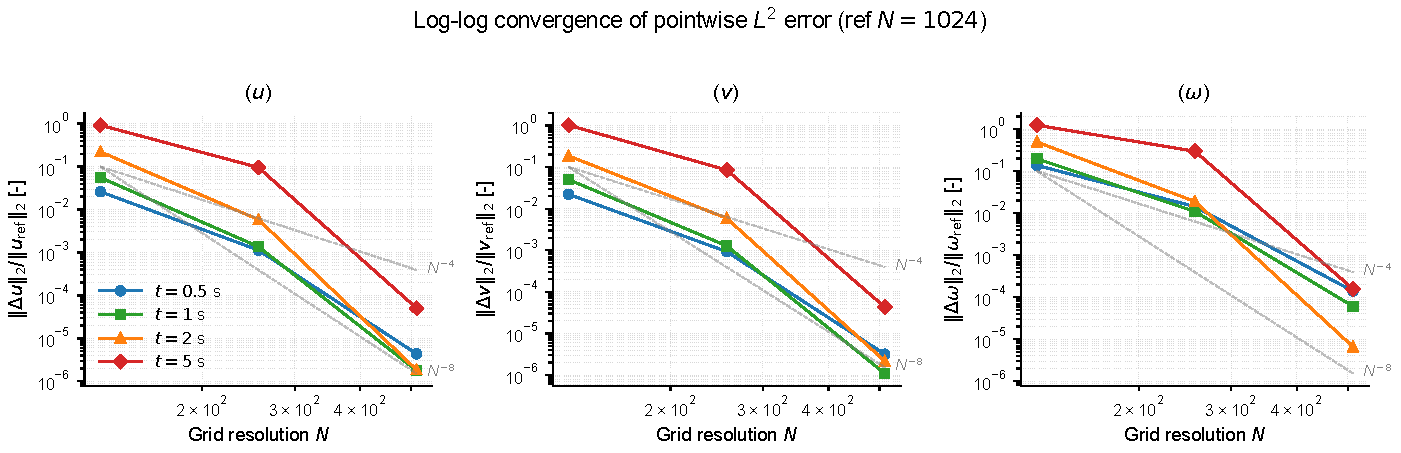
\includegraphics[width=\textwidth]{figures/results/grid_indep_supp_loglog.pdf}
    \caption{Log-log pointwise $L^2$ convergence against the $N=1024$ reference for the four-grid sweep at $Re=10^4$, evaluated at $t \in \{0.5, 1, 2, 5\}$~s. Each panel reports one field ($u$, $v$, $\omega$); dashed grey lines mark the algebraic reference slopes $N^{-4}$ and $N^{-8}$. Short-time slopes ($t \le 2$~s) lie steeper than $N^{-8}$, characteristic of pseudo-spectral super-algebraic convergence on a smooth IC; the $t=5$~s slope is shallower because pointwise error late in the chaotic trajectory is bounded by chaos amplification rather than discretisation truncation (statistical metrics in Fig.~\ref{fig:grid_indep_main}(a) remain at $0.064\%$).}
    \label{fig:grid_indep_supp_loglog}
\end{figure}

\begin{figure}[!htbp]
    \centering
    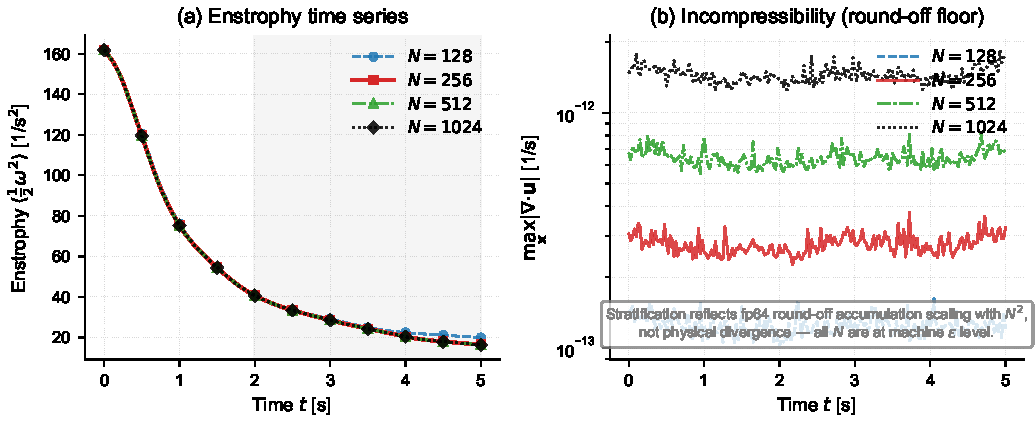
\includegraphics[width=\textwidth]{figures/results/grid_indep_supp_enstrophy_div.pdf}
    \caption{Secondary time-series diagnostics for the four-grid sweep. (a) Enstrophy $\langle \omega^2/2 \rangle(t)$; $N \ge 256$ overlap throughout, with the post-spin-up window ($t \ge 2$~s) shaded. (b) Maximum spectral incompressibility $\max_{\mathbf{x}} |\nabla \cdot \mathbf{u}|(t)$. All four grids sit at the fp64 round-off floor ($<10^{-11}$~1/s throughout); the apparent stratification reflects round-off accumulation scaling with $N^2$ over $\sim 10^5$ time steps rather than physical divergence.}
    \label{fig:grid_indep_supp_enstrophy_div}
\end{figure}


\chapter{Pressure-Field Scope Limit}
\label{app:pressure_limit}

Per the engineering-deployable regime (\S\ref{sec:engineering_constraint}, supervision condition~1) and the channel-availability assumption (\S\ref{sec:assumptions}), the network outputs $p$ as a model-internal variable without direct supervision. The momentum residual couples $p$ to the loss only through $\nabla p$; $p$ itself carries an additive gauge ($p\to p+C(t)$ leaves the dynamics unchanged). This appendix quantifies how far the resulting internal pressure departs from the DNS reference.

\paragraph{Pressure-gradient metric.}
The physically meaningful comparison is the pressure-gradient relative $L_2$ error
\begin{equation}
    \mathrm{p}^{\nabla}_{\rm rel\,L_2}(t) \;=\; \frac{\big\Vert \nabla p_{\rm pred}(t) - \nabla p_{\rm DNS}(t)\big\Vert_2}{\Vert \nabla p_{\rm DNS}(t)\Vert_2},
\end{equation}
computed by central finite differences on the $128^2$ evaluation grid. A gauge-removed pressure-value error
$p_{\rm rel\,L_2}^{\rm GR}(t) = \Vert p_{\rm pred}^{\rm GR}-p_{\rm DNS}^{\rm GR}\Vert_2/\Vert p_{\rm DNS}^{\rm GR}\Vert_2$
(with $p^{\rm GR} = p - \langle p\rangle_{\Omega}$) serves as a secondary diagnostic.

\begin{table}[!htbp]
    \centering
    \caption{Pressure-gradient (units: $\mathrm{m}/\mathrm{s}^2$) and gauge-removed pressure (units: $\mathrm{m}^2/\mathrm{s}^2$) metrics on the two reference configurations ($128^2$ evaluation grid, time-mean). Relative-error entries are dimensionless percentages.}
    \label{tab:pressure_limit}
    \footnotesize
    \setlength{\tabcolsep}{4pt}
    \begin{tabular}{lcccc}
    \toprule
    \textbf{Configuration} & $\mathrm{p}^{\nabla}_{\rm rel\,L_2}$ & $\Vert\nabla p\Vert_{\rm rms}^{\rm pred}$ & $\Vert\nabla p\Vert_{\rm rms}^{\rm DNS}$ & $p_{\rm rel\,L_2}^{\rm GR}$ (diag.) \\
    \midrule
    No-AL reference        & $112.0\%$ & $2.14$ & $7.63$ & $117.8\%$ \\
    AL main ($\rho=0.1$)   & $111.2\%$ & $2.10$ & $7.63$ & $119.7\%$ \\
    \bottomrule
    \end{tabular}
\end{table}

\paragraph{Reading.}
The two configurations give near-identical numbers: predicted $\Vert\nabla p\Vert_{\rm rms}$ is $\sim 28\%$ of the DNS reference, and $\mathrm{p}^{\nabla}_{\rm rel\,L_2}\sim 112\%$. The result is independent of the AL recipe and consistent with the stated regime: the momentum residual underdetermines $\nabla p$, since any smooth pattern partially cancelling $(\mathbf{u}\cdot\nabla)\mathbf{u}$ is admissible. The velocity field $(u,v)$ remains physically meaningful (\S\ref{sec:main_result}), with divergence driven to the band-limited finite-difference floor of its resolved scales (\S\ref{sec:sub_dns_div}) and accurate forcing-mode amplitude/phase (\S\ref{sec:spectrum}); downstream pressure reconstruction lies outside the present scope. Restoring pressure consistency requires either a sparse pressure-tap channel or an architectural reparametrization (pressure-Poisson decoder), listed as future work in \S\ref{sec:future_work}.

\chapter{Training Convergence Diagnostics}
\label{app:training_convergence}

This appendix documents the optimization dynamics of the main pipeline configuration (LES-derived placement, $1024$ collocation points, $20\,000$ iterations, seed 42; Table~\ref{tab:main_metrics}), complementing the loss and optimizer description of \S\ref{sec:loss}--\S\ref{sec:optimization}.

Figure~\ref{fig:opt_diagnostics} reports three diagnostics over training. The loss components decrease and plateau. The four GradNorm task weights, initialized at $[1, 0.057, 0.057, 0.01]$ for $[\mathrm{data}, \mathrm{NS}_u, \mathrm{NS}_v, \mathrm{cont}]$, rebalance toward $[1.00, 0.72, 0.79, 0.77]$ as the physics-residual gradients shrink relative to the data term. The Augmented-Lagrangian dual $\lambda_{\rm cont}$ grows monotonically to $0.39$ while the mean-squared continuity residual EMA $\tilde{C}_{\rm ema}$ relaxes toward zero, confirming that the continuity constraint is actively enforced through the dual ascent of \S\ref{subsec:al_cont} rather than only penalized.

\begin{figure}[!htbp]
    \centering
    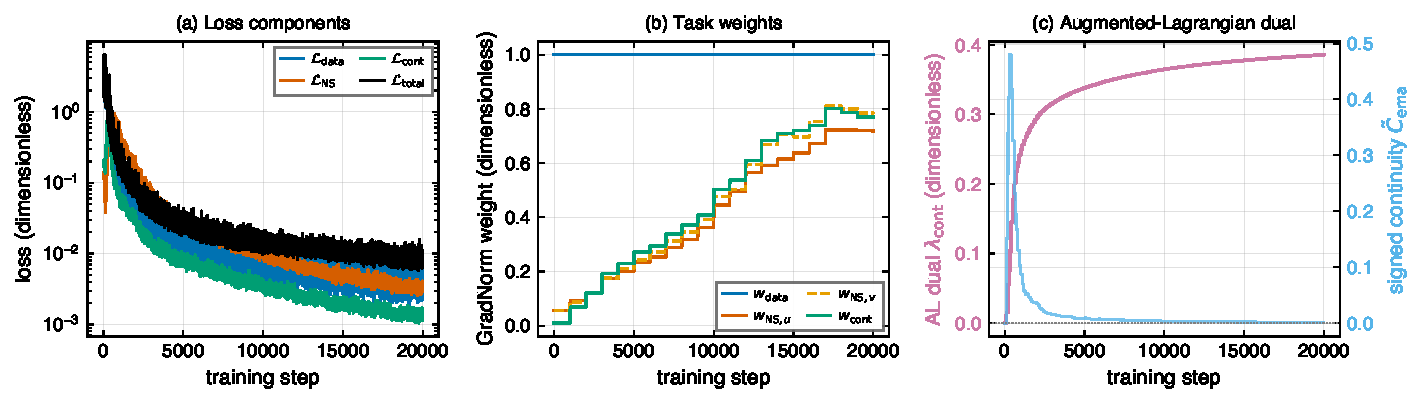
\includegraphics[width=\linewidth]{figures/results/optimization_diagnostics.pdf}
    \caption{Training convergence diagnostics for the main pipeline (seed 42, $20\,000$ iterations). (a) Loss components (dimensionless) versus training step, log scale. (b) GradNorm task weights (dimensionless) versus training step. (c) Augmented-Lagrangian dual $\lambda_{\rm cont}$ (left axis, dimensionless) and mean-squared continuity residual EMA $\tilde{C}_{\rm ema}$ (right axis) versus training step.}
    \label{fig:opt_diagnostics}
\end{figure}

\chapter{Information-Ceiling and Falsifiability Diagnostics}
\label{app:info_ceiling_diagnostics}

\section{Information-Theoretic Ceiling}
\label{sec:info_limit}

Three architecture-independent diagnostics quantify the $K=100$ sensor information limit. The wavelet sparsity diagnostic (Table~\ref{tab:wavelet}) yields Gini $\approx 0.985$ for $u, v$; $99\%$ of energy concentrates in $\sim 328$ of $65\,536$ coefficients ($s/N \approx 0.5\%$). The CS bound \eqref{eq:cs_bound} then gives
\begin{equation}
    M \;\gtrsim\; C_0 \cdot 328 \cdot \log_2(65\,536/328) \;\in\; [2\,500, 5\,000] \quad (C_0\in[1,2]),
\end{equation}
so $K=100$ covers the approximation band ($\sim 196$ coefficients, $94.4\%$ energy) but lies below the CS threshold for mid/high-band detail coefficients. A 2D Fourier basis yields comparable Gini values and the same $\mathcal{O}(s\log_2 N)$ scaling ($M^*=2\,506$ for $C_0=1$); the wavelet-sparsity algorithm is given below.

\begin{table}[!htbp]
    \centering
    \caption{Wavelet sparsity diagnostic on $u, v$ (m/s) and vorticity $\omega$ (1/s) at $t=5$ (db4 2-D wavelet transform). Sparsity threshold $s$ is the number of coefficients carrying $99\%$ of the energy.}
    \label{tab:wavelet}
    \small
    \begin{tabular}{lccc}
    \toprule
    \textbf{Field} & \textbf{Gini coefficient} & \textbf{99\%-energy coefficients} & \textbf{Fraction of total} \\
    \midrule
    $u$ & 0.983 & 326 & 0.50\% \\
    $v$ & 0.985 & 330 & 0.50\% \\
    $\omega$ & 0.942 & 1\,917 & 2.92\% \\
    \bottomrule
    \end{tabular}
\end{table}

\paragraph{Wavelet sparsity algorithm.}
The diagnostic applies, for each $u(t,\cdot)$ and $v(t,\cdot)$: (i) a 5-level db4 2D wavelet decomposition; (ii) coefficients flattened and sorted by absolute value; (iii) a cumulative-energy curve $E_p = \sum_{i\le p} c_i^2 / \sum_i c_i^2$, taking $p^*$ with $E_{p^*}\ge 0.99$; and (iv) the Gini coefficient $G = \frac{2\sum_i i\,c_i}{N\sum_i c_i} - \frac{N+1}{N}$ (with $\{c_i\}$ in ascending $|c|$). Values appear in Table~\ref{tab:wavelet}.

\paragraph{Null-space dimension via sensing SVD.}
A complementary measure counts how many divergence-free Fourier modes the $K=100$ sensors directly constrain. Parameterising the field by its stream function and truncating at $|\mathbf{k}|\le 16$ gives $M = 796$ real degrees of freedom; the sensing matrix $A\in\mathbb{R}^{200\times 796}$ maps these to the $2K=200$ scalar $(u,v)$ measurements. SVD gives $\mathrm{rank}(A) = 200$ (smallest singular value $\approx 497$, well above noise), so the null-space fraction within the $k\le 16$ truncation is $(796-200)/796 = 74.9\%$. In the approximation band ($M=196$, $k\lesssim 8$, the largest $M<2K$ on a 2D radial grid), every divergence-free mode is linearly observable ($\mathrm{rank}(A)=196$). Conditioning still degrades sharply across this band: $\kappa\approx 7$ for $k\le 5$ versus $\kappa\approx 7\times 10^{2}$ for $k\le 8$, so modes near $k\lesssim 8$ are observable but strongly noise-amplifying. The effective reconstructable bandwidth is therefore set by conditioning and noise rather than a hard observability wall, consistent with the achieved effective cutoff $k_{\rm cut}\approx 4.7$ lying inside the $k\lesssim 8$ ceiling.

A complementary spectral-truncation bound assumes perfect reconstruction up to cutoff $k_{\rm cut}$; the residual KE and $\omega$ errors are then architecture-independent (Table~\ref{tab:spectral_truncation}). The $K=100$ sensor Nyquist gives $k_{\max}^{\rm sensor} = \sqrt{K/\pi} \approx 5.64$.

\begin{table}[!htbp]
    \centering
    \caption{Spectral-truncation lower bound: residual KE and vorticity relative error after perfect reconstruction up to cutoff $k_{\rm cut}$.}
    \label{tab:spectral_truncation}
    \small
    \setlength{\tabcolsep}{8pt}
    \begin{tabular}{ccc}
    \toprule
    \textbf{$k_{\rm cut}$} & \textbf{KE loss \%} & \textbf{$\omega$ rel-$L_2$ \%} \\
    \midrule
    4  & $7.77$ & $63.91$ \\
    5  & $4.85$ & $57.18$ \\
    6  & $2.62$ & $51.07$ \\
    8  & $1.05$ & $40.98$ \\
    16 & $0.09$ & $20.96$ \\
    \bottomrule
    \end{tabular}
\end{table}

\paragraph{Ceiling attribution.}
The B3 multi-seed KE error (Table~\ref{tab:multiseed}, $5.71\%$) sits between the $k_{\rm cut}=4$ ($7.77\%$) and $k_{\rm cut}=5$ ($4.85\%$) bounds, mapping to effective cutoff $k_{\rm cut}\approx 4.7$; the vorticity error ($41.79\%$) sits between the $k_{\rm cut}=6$ ($51.07\%$) and $k_{\rm cut}=8$ ($40.98\%$) bounds, mapping to $k_{\rm cut}\approx 7.8$, at the upper edge of the $k\lesssim 8$ linear-observability band identified above. The two metrics bracket the effective bandwidth rather than agreeing on one value, as follows from fitting a single sharp-cutoff model to an energy-weighted and a $k^2$-weighted error in turn. The residual mid/high-band error is consistent with the sensor-information limit at this budget: reducing it requires more sensors rather than changes to architecture, optimizer, or loss (\S\ref{sec:engineering_app}).

\chapter{Boundary Diagnostics and Interpolation Baselines}
\label{app:diagnostic_ablation_forward_cfd}

\section{Boundary Diagnostics}
\label{sec:diagnostics}

The diagnostics below define what the final recipe does \emph{not} claim. They are single-seed or local-sweep checks under the final LES-pivot, $1024$-collocation, $20\,000$-iteration protocol unless otherwise noted, and are therefore used to set boundaries rather than to support Chapter~\ref{ch:results} main evidence.

\begin{table}[!htbp]
    \centering
    \caption{Boundary diagnostics for alternative recipe choices at $Re=10\,000$, $K=100$. Metrics are percentages unless noted. The multi-seed main baseline remains $5.71 \pm 0.12\%$ KE error.}
    \label{tab:boundary_diagnostics}
    \footnotesize
    \setlength{\tabcolsep}{3pt}
    \renewcommand{\arraystretch}{1.08}
    \begin{tabularx}{\textwidth}{p{2.6cm}p{4.6cm}p{3.2cm}X}
    \toprule
    \textbf{Diagnostic} & \textbf{Probe} & \textbf{Observed range} & \textbf{Reading} \\
    \midrule
    Multi-constraint AL
    & Add AL terms to NS momentum and/or continuity, with alternative GradNorm task sets.
    & KE $5.47$--$6.31$; div ratio $0.39$--$0.57$.
    & NS-momentum AL is not categorically unstable, but the effect is a divergence--accuracy trade-off rather than a validated improvement. \\
    \midrule
    Continuity-AL strength
    & Vary $\rho$ around the main $\rho=0.1$ setting: $0.03$, $0.30$, $1.00$.
    & KE $5.88$--$6.12$; div ratio decreases $0.45 \to 0.28$.
    & Larger $\rho$ tightens divergence but costs field accuracy; $\rho$ is a physics--data knob, not a source of improved reconstruction. \\
    \midrule
    Forcing recovery
    & Learn $A$, $k_f$, or both from near-zero initialisation ($A_{\rm init}=0.001$, $k_{f,\rm init}=0.01$).
    & Learned values collapse near $A=0.001$, $k_f=0.01$ while KE stays $5.74$--$5.85$.
    & Accurate velocity reconstruction does not certify recovery of the forcing parameters; structural identifiability is not established. \\
    \midrule
    Filtering vs.\ smoothing
    & Compare deployable filtering against offline bidirectional smoothing.
    & Filtering KE $5.71 \pm 0.12$; smoothing KE $5.74$.
    & Future-sensor access gives no clear gain in this single-seed diagnostic; filtering remains the deployable default. \\
    \bottomrule
    \end{tabularx}
\end{table}

\paragraph{Recipe implication.}
The final pipeline therefore keeps continuity-only AL with $\rho=0.1$, fixed forcing parameters, and filtering-mode CfC. These choices are conservative: they are supported by the $n=5$ main baseline, avoid non-deployable future-sensor access, and do not promote single-seed alternatives into recipe claims.

\paragraph{Detailed diagnostic anchors.}
\label{sec:multi_al_negative}
\label{sec:al_strength_appendix}
\label{sec:forcing_identifiability}
\label{sec:filtering_smoothing}
Table~\ref{tab:boundary_diagnostics} is the canonical summary for the diagnostic boundary cases referenced from Chapter~\ref{ch:results} and Chapter~\ref{ch:discussion_conclusion}.

\section{Engineering-Transferable Interpolation Baselines}
\label{app:fair_baselines}

Three classical reconstructions respect the same sensor-only constraint as PI-CON (no DNS access at training or inference): radial basis function (RBF) interpolation with a multiquadric kernel, inverse distance weighting (IDW), and a divergence-free trigonometric least-squares fit on a truncated Fourier basis ($k_{\max}=5$, matching the $K=100$ Nyquist scale). Table~\ref{tab:fair_baselines} compares them with PI-CON on the same $K=100$ LES-derived sensors used for the main baseline, so the comparison isolates the reconstruction method at a fixed sensor placement. The RBF shape parameter ($\varepsilon=10$, of order one sensor spacing) and the truncation ($k_{\max}=5$, the $K=100$ Nyquist scale) are fixed from these a-priori scales rather than tuned to minimise DNS error, keeping the baselines sensor-only.

\begin{table}[!htbp]
    \centering
    \caption{Engineering-transferable interpolation baselines vs.\ PI-CON at $Re=10\,000$, $K=100$ (same $K=100$ LES-derived sensors as the main baseline, no DNS access). PI-CON: mean $\pm$ standard deviation over $n=5$ seeds. Rightmost column: PI-CON relative reduction in $u$ rel-$L_2$. Relative-error metrics are percentages.}
    \label{tab:fair_baselines}
    \footnotesize
    \setlength{\tabcolsep}{3pt}
    \begin{tabular}{lccccc}
    \toprule
    \textbf{Method} & \textbf{KE \%} & \textbf{$u$ $L_2$ \%} & \textbf{$v$ $L_2$ \%} & \textbf{$\omega$ $L_2$ \%} & \textbf{$u$-$L_2$ rel.\ red.} \\
    \midrule
    RBF multiquadric ($\varepsilon=10$)   & $5.08$  & $30.02$ & $34.43$ & $58.33$ & $54.5\%$ \\
    IDW ($p=2$)                           & $66.66$ & $52.88$ & $62.02$ & $81.89$ & $74.2\%$ \\
    Div-free trig.\ LSQ ($k_{\max}=5$)    & $4.42$  & $25.87$ & $31.96$ & $63.41$ & $47.2\%$ \\
    \midrule
    \textbf{PI-CON (ours, $n=5$)}         & $5.71 {\pm} 0.12$ & $\mathbf{13.65 {\pm} 0.06}$ & $\mathbf{17.52 {\pm} 0.10}$ & $\mathbf{41.77 {\pm} 0.12}$ & -- \\
    \bottomrule
    \end{tabular}
\end{table}

\paragraph{Kinetic energy is a misleading sole metric.}
RBF multiquadric and the divergence-free trigonometric least-squares post lower KE error ($5.08\%$ and $4.42\%$) than the PI-CON multi-seed mean ($5.71\%$), but both reconstruct the field markedly worse pointwise. Classical interpolation contracts the velocity toward the inter-sensor mean, suppressing total kinetic energy and collapsing the KE ratio toward the DNS value for the wrong reason; the pointwise $u$- and $v$-$L_2$ rows expose this. PI-CON reduces $u$ rel-$L_2$ by $47.2\%$ relative to the strongest fair baseline (trigonometric LSQ, $25.87\%\to13.65\%$) and by $74.2\%$ relative to IDW. Pointwise error, rather than KE alone, separates reconstruction from energy contraction.

The refreshed interpolation sweep also shows strong hyperparameter sensitivity: under the same sensors, over-complete trigonometric LSQ at $k_{\max}=8$ and $12$ and poorly chosen RBF length scales can produce errors orders of magnitude larger than the carefully selected rows in Table~\ref{tab:fair_baselines}. These unstable variants are excluded from the main comparison table and treated as evidence that classical interpolation baselines require explicit validation rather than default trust.



\end{CJK}
\end{document}
